\documentclass[twoside]{book}

% Packages required by doxygen
\usepackage{fixltx2e}
\usepackage{calc}
\usepackage{doxygen}
\usepackage[export]{adjustbox} % also loads graphicx
\usepackage{graphicx}
\usepackage[utf8]{inputenc}
\usepackage{makeidx}
\usepackage{multicol}
\usepackage{multirow}
\PassOptionsToPackage{warn}{textcomp}
\usepackage{textcomp}
\usepackage[nointegrals]{wasysym}
\usepackage[table]{xcolor}

% Font selection
\usepackage[T1]{fontenc}
\usepackage[scaled=.90]{helvet}
\usepackage{courier}
\usepackage{amssymb}
\usepackage{sectsty}
\renewcommand{\familydefault}{\sfdefault}
\allsectionsfont{%
  \fontseries{bc}\selectfont%
  \color{darkgray}%
}
\renewcommand{\DoxyLabelFont}{%
  \fontseries{bc}\selectfont%
  \color{darkgray}%
}
\newcommand{\+}{\discretionary{\mbox{\scriptsize$\hookleftarrow$}}{}{}}

% Page & text layout
\usepackage{geometry}
\geometry{%
  a4paper,%
  top=2.5cm,%
  bottom=2.5cm,%
  left=2.5cm,%
  right=2.5cm%
}
\tolerance=750
\hfuzz=15pt
\hbadness=750
\setlength{\emergencystretch}{15pt}
\setlength{\parindent}{0cm}
\setlength{\parskip}{3ex plus 2ex minus 2ex}
\makeatletter
\renewcommand{\paragraph}{%
  \@startsection{paragraph}{4}{0ex}{-1.0ex}{1.0ex}{%
    \normalfont\normalsize\bfseries\SS@parafont%
  }%
}
\renewcommand{\subparagraph}{%
  \@startsection{subparagraph}{5}{0ex}{-1.0ex}{1.0ex}{%
    \normalfont\normalsize\bfseries\SS@subparafont%
  }%
}
\makeatother

% Headers & footers
\usepackage{fancyhdr}
\pagestyle{fancyplain}
\fancyhead[LE]{\fancyplain{}{\bfseries\thepage}}
\fancyhead[CE]{\fancyplain{}{}}
\fancyhead[RE]{\fancyplain{}{\bfseries\leftmark}}
\fancyhead[LO]{\fancyplain{}{\bfseries\rightmark}}
\fancyhead[CO]{\fancyplain{}{}}
\fancyhead[RO]{\fancyplain{}{\bfseries\thepage}}
\fancyfoot[LE]{\fancyplain{}{}}
\fancyfoot[CE]{\fancyplain{}{}}
\fancyfoot[RE]{\fancyplain{}{\bfseries\scriptsize Generated by Doxygen }}
\fancyfoot[LO]{\fancyplain{}{\bfseries\scriptsize Generated by Doxygen }}
\fancyfoot[CO]{\fancyplain{}{}}
\fancyfoot[RO]{\fancyplain{}{}}
\renewcommand{\footrulewidth}{0.4pt}
\renewcommand{\chaptermark}[1]{%
  \markboth{#1}{}%
}
\renewcommand{\sectionmark}[1]{%
  \markright{\thesection\ #1}%
}

% Indices & bibliography
\usepackage{natbib}
\usepackage[titles]{tocloft}
\setcounter{tocdepth}{3}
\setcounter{secnumdepth}{5}
\makeindex

% Hyperlinks (required, but should be loaded last)
\usepackage{ifpdf}
\ifpdf
  \usepackage[pdftex,pagebackref=true]{hyperref}
\else
  \usepackage[ps2pdf,pagebackref=true]{hyperref}
\fi
\hypersetup{%
  colorlinks=true,%
  linkcolor=blue,%
  citecolor=blue,%
  unicode%
}

% Custom commands
\newcommand{\clearemptydoublepage}{%
  \newpage{\pagestyle{empty}\cleardoublepage}%
}

\usepackage{caption}
\captionsetup{labelsep=space,justification=centering,font={bf},singlelinecheck=off,skip=4pt,position=top}

%===== C O N T E N T S =====

\begin{document}

% Titlepage & ToC
\hypersetup{pageanchor=false,
             bookmarksnumbered=true,
             pdfencoding=unicode
            }
\pagenumbering{alph}
\begin{titlepage}
\vspace*{7cm}
\begin{center}%
{\Large Arduino\+Menu 5 }\\
\vspace*{1cm}
{\large Generated by Doxygen 1.8.13}\\
\end{center}
\end{titlepage}
\clearemptydoublepage
\pagenumbering{roman}
\tableofcontents
\clearemptydoublepage
\pagenumbering{arabic}
\hypersetup{pageanchor=true}

%--- Begin generated contents ---
\chapter{Arduino\+Menu 5 documentation}
\label{index}\hypertarget{index}{}\hypertarget{index_intro_sec}{}\section{Introduction}\label{index_intro_sec}
Generic interactive system for embedded devices and small systems\hypertarget{index_install_sec}{}\section{Installation}\label{index_install_sec}
\hypertarget{index_arduino_libs}{}\subsection{From Arduino-\/\+I\+DE}\label{index_arduino_libs}
search for Arduino\+Menu by Rui Azevedo\hypertarget{index_platformio_libs}{}\subsection{From Platformio}\label{index_platformio_libs}
search for Arduino\+Menu on platformio Home-\/$>$Libraries 
\chapter{Arduino\+Menu 5}
\label{md_README}
\Hypertarget{md_README}
{\bfseries Generic menu/interactivity system for the arduino framework}

\subsection*{Development discussion about next menu version}

This is an experimental area, please contribute with ideas, experience or code. Thank you.

\subsubsection*{Why a new version}

In a word, {\bfseries size}.

Things I wish were available\+:
\begin{DoxyItemize}
\item C++14 or +
\item A\+VR stl
\end{DoxyItemize}

\subsection*{Current state}

{\itshape tiny.\+ino} example is using a single option print-\/out chain

with composing menu items, role description tags and role tag catch on output format

output is also a composition, we can compose role tag format handlers and translations.


\begin{DoxyCode}
\{c++\}
// Rui Azevedo - Apr2019
// neu-rah (ruihfazevedo@gmail.com)
// LCD example with flash data (Arduino framework)
//
// ArduinoMenu libtary 5.x code example
// Output: LCD
// flash data
// Input: user serial driver

#include <menu/def/tinyArduino.h>
#include <menu/IO/lcdOut.h>

using namespace Menu;

// LCD /////////////////////////////////////////
#define RS 2
#define RW 4
#define EN A4
LiquidCrystal lcd(RS, RW, EN, A0, A1, A2, A3);

//menu output ------------------------
MenuOut<AM5::LCDFmt<>::To<LCDOutDev<lcd>>> menuOut;

using Op=Prompt<FlashText>;

const char op1\_text[] PROGMEM="Op 1";
Op op1(op1\_text);

const char op2\_text[] PROGMEM="Op 2";
Op op2(op2\_text);

const char op3\_text[] PROGMEM="Op 3";
Op op3(op3\_text);

const char op4\_text[] PROGMEM="Op 4";
Op op4(op4\_text);

const char op5\_text[] PROGMEM="Op 5";
Op op5(op5\_text);

// Prompt<StaticMenu<5>> mainMenu("Main menu",&op1,&op2,&op3,&op4,&op5);
const char menuTitle\_text[] PROGMEM="Main menu";
Op menuTitle(menuTitle\_text);
constexpr AM5::FlashData data[5] \{&op1,&op2,&op3,&op4,&op5\};
Prompt<AM5::FlashMenuDef<data,5,FlashText>> mainMenu(menuTitle\_text);

void setup() \{
  Serial.begin(115200);
  while(!Serial);
  lcd.begin(16,2);
  menuOut<<F("AM5 example ----")<<endl;
  menuOut<<F("<www.r-site.net>")<<endl;
  delay(1500);
  lcd.clear();
  menuOut.setTarget(mainMenu);
  menuOut.printMenu();
\}

//handle serial keys to navigate menu
bool keys(int key) \{
  switch(key) \{
    case '+': return menuOut.up();;
    case '-': return menuOut.down();;
    case '*': return menuOut.enter();;
    case '/': return menuOut.esc();;
  \}
  return false;
\}

void loop() \{
  if (Serial.available()) \{
    if (keys(Serial.read())) menuOut.printMenu();
  \}
\}
\end{DoxyCode}


{\bfseries footprint\+:} 
\begin{DoxyCode}
current:
ATA:    [==        ]  18.3% (used 374 bytes from 2048 bytes)
PROGRAM: [==        ]  15.3% (used 4704 bytes from 30720 bytes)

previous:
DATA:    [==        ]  19.1% (used 392 bytes from 2048 bytes)
PROGRAM: [==        ]  17.1% (used 5242 bytes from 30720 bytes)
\end{DoxyCode}


{\itshape tiny\+Arduino.\+h} defines {\ttfamily \hyperlink{structSerialOut}{Serial\+Out}}, {\ttfamily Op} and {\ttfamily Flash\+Op} as\+: 
\begin{DoxyCode}
\{c++\}
#include <streamFlow.h>//https://github.com/neu-rah/streamFlow
#include "../../menu.h"
#include "../printers.h"
#include "../comp/flashText.h"
#include "../comp/flashMenu.h"

namespace Menu \{

  using namespace Menu;

  template<typename O>
  using MenuOut=AM5::MenuOutCap<O>;

  using FlashText=AM5::FlashTextDef<AM5::Empty>;

  using Text=AM5::Text<AM5::Empty>;

  using Item=AM5::Item;

  template<typename O>
  using Prompt=AM5::Prompt<O>;

  template<size\_t n>
  using StaticMenu=AM5::StaticMenu<n,Text>;

  template<size\_t n>
  using FlashMenu=AM5::StaticMenu<n,FlashText>;
\};
\end{DoxyCode}


\href{https://gitter.im/ArduinoMenu/Lobby}{\tt https\+://gitter.\+im/\+Arduino\+Menu/\+Lobby}

\subsubsection*{Embedded systems}

The A\+M4 approach to library development is not sufficient for embedded systems, modularity by includes is not enough as a means of optimization. As we start adding features soon the menu becomes tight on small devices. So we need to seek modularity even further.

After some research and experimentation here are some considerations about various aspects of menu systems with focus on embedding.

This can also be achieved with C style defines and code exclusion, both approaches are hard. Hopefully this one can be more succinct.

\subsubsection*{Is it possible?}

You might be using a single line display, therefore printing a menu title is useless and inconvenient. instead of having a run-\/time config and code checking if title enabled and skipping title prints on single line devices even if active make a menu system easy to use but also makes it heavier. Examples like this are behind all assumptions we make about a menu system. So instead of having extra runtime check/config we opt instead on having compile-\/time compositions, think it like, if you want the title on your menus you can simply include that part on the construct. Shifting the burden to compile time reduces the run-\/time checking, code size and increases speed.

{\itshape {\bfseries technical\+:} using type to guide the composition decision, not used code vanish at compile time.}

\paragraph*{Mixed content}

Instead of setting a menu structure to reside on flash or on ram we can use them mixed. And this is working.

\paragraph*{No assumptions}

Assumptions reveal most of the time, a trade or a burden, assuming that all prompts/options will have a text might not be correct, useful or sufficient, some systems might need multiple texts for multi-\/language. Same goes to all assumptions about menus, even associated actions.

\paragraph*{Composition (type level)}

The key to obtain better modularity is by code composition using C++ mixins.

We make type level compositions that define a menu system type. That can be adequate for simple or complex system.

\subparagraph*{How things compose}

Composition is done at type level using templates and open derivation chain, this is quite loose but this level is not intended for the final user, still it allow a great customization.

It would be useless if we could not escape the type level. We want this different options of different type to co-\/exist on the same list. Therefor the interface usage. It defines a base menu item and its behavior.

Even not being enforced by C++ we adopted an interface description with a middle composing stage comprised of multiple classes/functionalities with inline static members, this kind of members tend to vanish if not used.

The composed types then are used to construct a specific version for the interface, virtual functions will ensure that the correct type is used covering the composition as a monolith type.

Some compositions are weight-\/less and therefor should be included always. That is the case of role description tags, all members should have one, they are transparent and no trace of them would be left, but they can influenciate the code generated for certain print devices or output formats if they, the format or device, choose to do so.

{\bfseries generic pattern}

Adapt(\+Interface)$<$Comp1$<$Comp2$<$Comp3$<$\+Terminal$>$$>$$>$$>$

```c++ //define common functionalities struct Interface \{ //some virtual functions here \};

//make static composition adhere to the interface (as a top level cap) template$<$typename O$>$ struct Adapt\+:public Interface,public O \{ //redirect virtual call to the correct type (because we know it) \};

// composition parts -\/-\/-\/-\/-\/-\/-\/-\/-\/-\/-\/-\/-\/-\/-\/-\/-\/-\/-\/---

//this is the minimal composition part and acts as an interface for the composing parts // however nothing requires you to derive from it as the members are {\ttfamily inline static} // consider it just a guide, deriving from it is a discipline struct \hyperlink{structEmpty}{Empty} \{ //add base functionality to derived items, not enforced but handy \};

template$<$typename o=\char`\"{}\+Empty\char`\"{}$>$ class Text\+:public O \{ protected\+: const char$\ast$ text; public\+: Text(const char$\ast$ t)\+:text(t) \{\} //... add specific implementations \};

//composing thing for user using Op=Prompt$<$\+Text$>$; //using Op=Prompt$<$\+Flash\+Text$>$;//with this def we can put all Op\textquotesingle{}s into flash (because they share constructor parameter format)

Op op1(\char`\"{}\+Op 1\char`\"{});//now we can simply build an option like this


\begin{DoxyCode}
we can implement other building blocks \_a la carte\_  
they contain the functionality and its code is vacuous if not used

we might add some sugar on top of this construction methods and build more elaborated blocks for each
       system.

**extending**

on a separate file, meaning the library can be extended without changing library files

```c++
  template<typename O>
  class FlashTextDef:public O \{
  protected:
    const char *text PROGMEM;
  public:
    FlashTextDef(PGM\_P t):text(t) \{\}
    template<typename Out>
    inline size\_t out(Out& o) \{
      o.raw(reinterpret\_cast<const \_\_FlashStringHelper *>(text));
      return O::out(o);//chain the call
    \}
  \};
\end{DoxyCode}


\subsubsection*{Lessons learned}

From previous version we have been adding functionalities and adapting the system design, however always over the same assumptions... Instead keep everything functional and interface contained.

Input manipulation should be independent, the system should only respond to navigation commands.

Output should be single device, multiple device should be implemented as a special device.

Finally found a decent initialization schema so that we can drop the macros (maybe keep them for compatibility/porting)

Target framework should not be limited to Arduino (essay on Linux went well)

Keep menu definitions platform agnostic as was on A\+M4, make them also framework agnostic.

On version 4 we shifted the complexity to a central core, this makes IO drivers easier to implement an is more efficient when using multiple outputs, but makes an extremely heavy core with many if\textquotesingle{}s and considering too many cases, we need to break this down. Type level composition was the way.

Avoid castings, macros and other bad style c++

Work at type level whenever possible 
\chapter{TO DO\+:}
\label{md_TODO}
\Hypertarget{md_TODO}
\subsection*{actions and events}


\begin{DoxyItemize}
\item ...
\end{DoxyItemize}

\subsection*{printers}


\begin{DoxyItemize}
\item invert printers composition order to be ontop of viewports
\item split \hyperlink{structFullPrinter}{Full\+Printer} into smaller printers
\end{DoxyItemize}

\subsection*{manage free/used space}


\begin{DoxyItemize}
\item panel-\/$>$viewport
\end{DoxyItemize}

viewport design


\begin{DoxyItemize}
\item viewport must sit between the printers and the raw device
\item keep track of space usage and position cursor accordingly
\item should allow creation of areas (new viewports) with special definitions =$>$ as a composition to be transparent
\item new views can be based on free area, to account for usage
\item support 2D scroll
\item they should ignore stuff outside the free viewport area before reaching the printer
\item measuring is taken here too
\item independent of menu structure or size, but must collaborate to adjust scroll position
\item use menu range to manage device panels
\item $\ast$$\ast$=$>$$\ast$$\ast$ need font size and glyph measure A\+PI, optionally account for U\+T\+F8, already inplace a minimal measure device (text)
\end{DoxyItemize}

\subsection*{tree nav}


\begin{DoxyItemize}
\item separate the base nav
\item use menu range to manage navigation levels
\end{DoxyItemize}

\subsection*{accelerators}


\begin{DoxyItemize}
\item optionally use a single table with actions
\end{DoxyItemize}

\subsection*{redraw need check}


\begin{DoxyItemize}
\item draw, calc and redraw need should have the same functional root
\end{DoxyItemize}

\subsection*{extra field types}


\begin{DoxyItemize}
\item redirect input commands to fields... but keep vtable small
\item implement text options for E\+E\+P\+R\+OM based data 
\end{DoxyItemize}
\chapter{Module Index}
\section{Modules}
Here is a list of all modules\+:\begin{DoxyCompactList}
\item \contentsline{section}{Menu items}{\pageref{group__Items}}{}
\begin{DoxyCompactList}
\item \contentsline{section}{Command and navigation agents}{\pageref{group__Agents}}{}
\end{DoxyCompactList}
\item \contentsline{section}{Navigation system}{\pageref{group__Navigation}}{}
\item \contentsline{section}{Menu output}{\pageref{group__Output}}{}
\item \contentsline{section}{Part printing}{\pageref{group__Printers}}{}
\end{DoxyCompactList}

\chapter{Hierarchical Index}
\section{Class Hierarchy}
This inheritance list is sorted roughly, but not completely, alphabetically\+:\begin{DoxyCompactList}
\item \+\_\+O\begin{DoxyCompactList}
\item \contentsline{section}{Chain$<$ OO $>$\+:\+:Links$<$ \+\_\+T, \+\_\+O, \+\_\+\+OO $>$}{\pageref{structChain_1_1Links}}{}
\item \contentsline{section}{Chain$<$ OO $>$\+:\+:Links$<$ \+\_\+T, \+\_\+O $>$}{\pageref{structChain_1_1Links_3_01__T_00_01__O_01_4}}{}
\item \contentsline{section}{Chain$<$ OO $>$\+:\+:Links$<$ T, OO... $>$}{\pageref{structChain_1_1Links}}{}
\begin{DoxyCompactList}
\item \contentsline{section}{Chain$<$ OO $>$\+:\+:To$<$ T $>$}{\pageref{structChain_1_1To}}{}
\end{DoxyCompactList}
\end{DoxyCompactList}
\item \contentsline{section}{Chain$<$ OO $>$}{\pageref{structChain}}{}
\item \contentsline{section}{Chain$<$ Text\+Fmt, Title\+Wrap, Full\+Printer, Viewport, Range\+Panel $>$}{\pageref{structChain}}{}
\item \contentsline{section}{Cmd\+Agent}{\pageref{structCmdAgent}}{}
\begin{DoxyCompactList}
\item \contentsline{section}{Empty\+Cmds$<$ res $>$}{\pageref{structEmptyCmds}}{}
\item \contentsline{section}{Empty\+Cmds$<$ false $>$}{\pageref{structEmptyCmds}}{}
\item \contentsline{section}{Empty\+Cmds$<$ true $>$}{\pageref{structEmptyCmds}}{}
\item \contentsline{section}{Item\+Cmd$<$ I, res $>$}{\pageref{structItemCmd}}{}
\item \contentsline{section}{Item\+Cmd$<$ Nav\+Handler $>$}{\pageref{structItemCmd}}{}
\end{DoxyCompactList}
\item I\begin{DoxyCompactList}
\item \contentsline{section}{Action$<$ I, act $>$}{\pageref{classAction}}{}
\item \contentsline{section}{As\+Mode$<$ I $>$}{\pageref{structAsMode}}{}
\item \contentsline{section}{As\+Unit$<$ I $>$}{\pageref{structAsUnit}}{}
\item \contentsline{section}{As\+Value$<$ I $>$}{\pageref{structAsValue}}{}
\item \contentsline{section}{Empty$<$ I $>$}{\pageref{structEmpty}}{}
\item \contentsline{section}{En\+Dis$<$ I $>$}{\pageref{classEnDis}}{}
\item \contentsline{section}{Flash\+Text$<$ T, text, I $>$}{\pageref{structFlashText}}{}
\item \contentsline{section}{Nav\+Handler$<$ I $>$}{\pageref{classNavHandler}}{}
\item \contentsline{section}{Num\+Field$<$ T, value, low, high, step, tune, I $>$}{\pageref{classNumField}}{}
\item \contentsline{section}{Prompt$<$ I $>$}{\pageref{structPrompt}}{}
\item \contentsline{section}{Static\+Menu$<$ I $>$}{\pageref{structStaticMenu_3_01I_01_4}}{}
\item \contentsline{section}{Static\+Text$<$ text, I $>$}{\pageref{structStaticText}}{}
\item \contentsline{section}{Vector\+Menu$<$ I $>$}{\pageref{structVectorMenu}}{}
\end{DoxyCompactList}
\item \contentsline{section}{Item}{\pageref{structItem}}{}
\begin{DoxyCompactList}
\item \contentsline{section}{Prompt$<$ I $>$}{\pageref{structPrompt}}{}
\end{DoxyCompactList}
\item \contentsline{section}{Menu\+Out}{\pageref{structMenuOut}}{}
\begin{DoxyCompactList}
\item \contentsline{section}{Menu\+Out\+Def$<$ O $>$}{\pageref{structMenuOutDef}}{}
\end{DoxyCompactList}
\item N\begin{DoxyCompactList}
\item \contentsline{section}{Drift$<$ N $>$}{\pageref{structDrift}}{}
\item \contentsline{section}{Item\+Nav$<$ N $>$}{\pageref{classItemNav}}{}
\item \contentsline{section}{Nav\+Base$<$ Out, N $>$}{\pageref{classNavBase}}{}
\begin{DoxyCompactList}
\item \contentsline{section}{Dynamic\+Nav$<$ Out, Data, N $>$}{\pageref{classDynamicNav}}{}
\item \contentsline{section}{Static\+Nav$<$ Out, Data, N $>$}{\pageref{classStaticNav}}{}
\end{DoxyCompactList}
\item \contentsline{section}{Nav\+Pos$<$ N $>$}{\pageref{classNavPos}}{}
\item \contentsline{section}{Nav\+Root$<$ N $>$}{\pageref{structNavRoot}}{}
\end{DoxyCompactList}
\item \contentsline{section}{Nav\+Agent}{\pageref{structNavAgent}}{}
\item \contentsline{section}{Nav\+Node}{\pageref{structNavNode}}{}
\begin{DoxyCompactList}
\item \contentsline{section}{Dynamic\+Nav$<$ Out, Data, N $>$}{\pageref{classDynamicNav}}{}
\end{DoxyCompactList}
\item \contentsline{section}{Nil}{\pageref{structNil}}{}
\begin{DoxyCompactList}
\item \contentsline{section}{Void$<$$>$}{\pageref{structVoid}}{}
\begin{DoxyCompactList}
\item \contentsline{section}{Text\+Measure}{\pageref{structTextMeasure}}{}
\end{DoxyCompactList}
\end{DoxyCompactList}
\item O\begin{DoxyCompactList}
\item \contentsline{section}{Liquid\+Crystal\+Out$<$ dev, O $>$}{\pageref{structLiquidCrystalOut}}{}
\item \contentsline{section}{Menu\+Out\+Def$<$ O $>$}{\pageref{structMenuOutDef}}{}
\item \contentsline{section}{Out\+List$<$ O $>$}{\pageref{classOutList_3_01O_01_4}}{}
\item \contentsline{section}{Range\+Panel$<$ O $>$}{\pageref{classRangePanel}}{}
\item \contentsline{section}{Raw\+Out$<$ Dev, dev, O $>$}{\pageref{structRawOut}}{}
\item \contentsline{section}{Raw\+Out$<$ Dev \&, dev, O $>$}{\pageref{structRawOut}}{}
\begin{DoxyCompactList}
\item \contentsline{section}{Serial\+Out$<$ Dev, dev, O $>$}{\pageref{structSerialOut}}{}
\end{DoxyCompactList}
\item \contentsline{section}{Raw\+Out$<$ ostream \&, dev, O $>$}{\pageref{structRawOut}}{}
\begin{DoxyCompactList}
\item \contentsline{section}{Console$<$ dev, O $>$}{\pageref{structConsole}}{}
\end{DoxyCompactList}
\item \contentsline{section}{Static\+Panel$<$ x, y, w, h, O $>$}{\pageref{structStaticPanel}}{}
\item \contentsline{section}{Text\+Fmt$<$ O $>$}{\pageref{structTextFmt}}{}
\item \contentsline{section}{Title\+Wrap\+Fmt$<$ O, open, close $>$}{\pageref{structTitleWrapFmt}}{}
\item \contentsline{section}{Viewport$<$ O $>$}{\pageref{classViewport}}{}
\item \contentsline{section}{Void$<$ O $>$}{\pageref{structVoid}}{}
\end{DoxyCompactList}
\item \contentsline{section}{Out\+List$<$ O, OO $>$}{\pageref{classOutList}}{}
\item \contentsline{section}{Out\+Op$<$ Out\+Ops $>$}{\pageref{structOutOp}}{}
\item P\begin{DoxyCompactList}
\item \contentsline{section}{Full\+Printer$<$ P $>$}{\pageref{structFullPrinter}}{}
\end{DoxyCompactList}
\item \contentsline{section}{Static\+Menu$<$ I, II $>$}{\pageref{classStaticMenu}}{}
\item vector\begin{DoxyCompactList}
\item \contentsline{section}{Vector\+Menu$<$ I $>$}{\pageref{structVectorMenu}}{}
\end{DoxyCompactList}
\end{DoxyCompactList}

\chapter{Class Index}
\section{Class List}
Here are the classes, structs, unions and interfaces with brief descriptions\+:\begin{DoxyCompactList}
\item\contentsline{section}{\hyperlink{classAction}{Action$<$ I, act $>$} }{\pageref{classAction}}{}
\item\contentsline{section}{\hyperlink{structAsMode}{As\+Mode$<$ I $>$} }{\pageref{structAsMode}}{}
\item\contentsline{section}{\hyperlink{structAsUnit}{As\+Unit$<$ I $>$} }{\pageref{structAsUnit}}{}
\item\contentsline{section}{\hyperlink{structAsValue}{As\+Value$<$ I $>$} }{\pageref{structAsValue}}{}
\item\contentsline{section}{\hyperlink{structChain}{Chain$<$ O\+O $>$} }{\pageref{structChain}}{}
\item\contentsline{section}{\hyperlink{structCmdAgent}{Cmd\+Agent} }{\pageref{structCmdAgent}}{}
\item\contentsline{section}{\hyperlink{structConsole}{Console$<$ dev, O $>$} }{\pageref{structConsole}}{}
\item\contentsline{section}{\hyperlink{structDrift}{Drift$<$ N $>$} }{\pageref{structDrift}}{}
\item\contentsline{section}{\hyperlink{classDynamicNav}{Dynamic\+Nav$<$ Out, Data, N $>$} }{\pageref{classDynamicNav}}{}
\item\contentsline{section}{\hyperlink{structEmpty}{Empty$<$ I $>$} }{\pageref{structEmpty}}{}
\item\contentsline{section}{\hyperlink{structEmptyCmds}{Empty\+Cmds$<$ res $>$} }{\pageref{structEmptyCmds}}{}
\item\contentsline{section}{\hyperlink{classEnDis}{En\+Dis$<$ I $>$} }{\pageref{classEnDis}}{}
\item\contentsline{section}{\hyperlink{structFlashText}{Flash\+Text$<$ T, text, I $>$} }{\pageref{structFlashText}}{}
\item\contentsline{section}{\hyperlink{structFullPrinter}{Full\+Printer$<$ P $>$} }{\pageref{structFullPrinter}}{}
\item\contentsline{section}{\hyperlink{structItem}{Item} }{\pageref{structItem}}{}
\item\contentsline{section}{\hyperlink{structItemCmd}{Item\+Cmd$<$ I, res $>$} }{\pageref{structItemCmd}}{}
\item\contentsline{section}{\hyperlink{classItemNav}{Item\+Nav$<$ N $>$} }{\pageref{classItemNav}}{}
\item\contentsline{section}{\hyperlink{structChain_1_1Links}{Chain$<$ O\+O $>$\+::\+Links$<$ \+\_\+\+T, \+\_\+\+O, \+\_\+\+O\+O $>$} }{\pageref{structChain_1_1Links}}{}
\item\contentsline{section}{\hyperlink{structChain_1_1Links_3_01__T_00_01__O_01_4}{Chain$<$ O\+O $>$\+::\+Links$<$ \+\_\+\+T, \+\_\+\+O $>$} }{\pageref{structChain_1_1Links_3_01__T_00_01__O_01_4}}{}
\item\contentsline{section}{\hyperlink{structLiquidCrystalOut}{Liquid\+Crystal\+Out$<$ dev, O $>$} }{\pageref{structLiquidCrystalOut}}{}
\item\contentsline{section}{\hyperlink{structMenuOut}{Menu\+Out} }{\pageref{structMenuOut}}{}
\item\contentsline{section}{\hyperlink{structMenuOutDef}{Menu\+Out\+Def$<$ O $>$} }{\pageref{structMenuOutDef}}{}
\item\contentsline{section}{\hyperlink{structNavAgent}{Nav\+Agent} }{\pageref{structNavAgent}}{}
\item\contentsline{section}{\hyperlink{classNavBase}{Nav\+Base$<$ Out, N $>$} }{\pageref{classNavBase}}{}
\item\contentsline{section}{\hyperlink{classNavHandler}{Nav\+Handler$<$ I $>$} }{\pageref{classNavHandler}}{}
\item\contentsline{section}{\hyperlink{structNavNode}{Nav\+Node} }{\pageref{structNavNode}}{}
\item\contentsline{section}{\hyperlink{classNavPos}{Nav\+Pos$<$ N $>$} }{\pageref{classNavPos}}{}
\item\contentsline{section}{\hyperlink{structNavRoot}{Nav\+Root$<$ N $>$} }{\pageref{structNavRoot}}{}
\item\contentsline{section}{\hyperlink{structNil}{Nil} }{\pageref{structNil}}{}
\item\contentsline{section}{\hyperlink{classNumField}{Num\+Field$<$ T, value, low, high, step, tune, I $>$} }{\pageref{classNumField}}{}
\item\contentsline{section}{\hyperlink{classOutList}{Out\+List$<$ O, O\+O $>$} }{\pageref{classOutList}}{}
\item\contentsline{section}{\hyperlink{classOutList_3_01O_01_4}{Out\+List$<$ O $>$} }{\pageref{classOutList_3_01O_01_4}}{}
\item\contentsline{section}{\hyperlink{structOutOp}{Out\+Op$<$ Out\+Ops $>$} }{\pageref{structOutOp}}{}
\item\contentsline{section}{\hyperlink{structPrompt}{Prompt$<$ I $>$} }{\pageref{structPrompt}}{}
\item\contentsline{section}{\hyperlink{classRangePanel}{Range\+Panel$<$ O $>$} }{\pageref{classRangePanel}}{}
\item\contentsline{section}{\hyperlink{structRawOut}{Raw\+Out$<$ Dev, dev, O $>$} }{\pageref{structRawOut}}{}
\item\contentsline{section}{\hyperlink{structSerialOut}{Serial\+Out$<$ Dev, dev, O $>$} }{\pageref{structSerialOut}}{}
\item\contentsline{section}{\hyperlink{classStaticMenu}{Static\+Menu$<$ I, I\+I $>$} }{\pageref{classStaticMenu}}{}
\item\contentsline{section}{\hyperlink{structStaticMenu_3_01I_01_4}{Static\+Menu$<$ I $>$} }{\pageref{structStaticMenu_3_01I_01_4}}{}
\item\contentsline{section}{\hyperlink{classStaticNav}{Static\+Nav$<$ Out, Data, N $>$} }{\pageref{classStaticNav}}{}
\item\contentsline{section}{\hyperlink{structStaticPanel}{Static\+Panel$<$ x, y, w, h, O $>$} }{\pageref{structStaticPanel}}{}
\item\contentsline{section}{\hyperlink{structStaticText}{Static\+Text$<$ text, I $>$} }{\pageref{structStaticText}}{}
\item\contentsline{section}{\hyperlink{structTextFmt}{Text\+Fmt$<$ O $>$} }{\pageref{structTextFmt}}{}
\item\contentsline{section}{\hyperlink{structTextMeasure}{Text\+Measure} }{\pageref{structTextMeasure}}{}
\item\contentsline{section}{\hyperlink{structTitleWrapFmt}{Title\+Wrap\+Fmt$<$ O, open, close $>$} }{\pageref{structTitleWrapFmt}}{}
\item\contentsline{section}{\hyperlink{structChain_1_1To}{Chain$<$ O\+O $>$\+::\+To$<$ T $>$} }{\pageref{structChain_1_1To}}{}
\item\contentsline{section}{\hyperlink{structVectorMenu}{Vector\+Menu$<$ I $>$} }{\pageref{structVectorMenu}}{}
\item\contentsline{section}{\hyperlink{classViewport}{Viewport$<$ O $>$} }{\pageref{classViewport}}{}
\item\contentsline{section}{\hyperlink{structVoid}{Void$<$ O $>$} }{\pageref{structVoid}}{}
\end{DoxyCompactList}

\chapter{File Index}
\section{File List}
Here is a list of all documented files with brief descriptions\+:\begin{DoxyCompactList}
\item\contentsline{section}{src/\hyperlink{menu_8h}{menu.\+h} \\*Arduino\+Menu main include file }{\pageref{menu_8h}}{}
\item\contentsline{section}{src/menu/\hyperlink{base_8h}{base.\+h} \\*Arduino\+Menu interfaces (A\+PI\textquotesingle{}s) }{\pageref{base_8h}}{}
\item\contentsline{section}{src/menu/{\bfseries base.\+hpp} }{\pageref{base_8hpp}}{}
\item\contentsline{section}{src/menu/\hyperlink{debug_8h}{debug.\+h} \\*Debug macros and utilities }{\pageref{debug_8h}}{}
\item\contentsline{section}{src/menu/\hyperlink{item_8h}{item.\+h} \\*Base menu item implementations }{\pageref{item_8h}}{}
\item\contentsline{section}{src/menu/\hyperlink{nav_8h}{nav.\+h} \\*Arduino\+Menu navigation implementations }{\pageref{nav_8h}}{}
\item\contentsline{section}{src/menu/\hyperlink{out_8h}{out.\+h} \\*Arduino\+Menu output implementations }{\pageref{out_8h}}{}
\item\contentsline{section}{src/menu/\hyperlink{panels_8h}{panels.\+h} \\*Arduino\+Menu output space management }{\pageref{panels_8h}}{}
\item\contentsline{section}{src/menu/\hyperlink{printers_8h}{printers.\+h} \\*Arduino\+Menu part printers }{\pageref{printers_8h}}{}
\item\contentsline{section}{src/menu/comp/\hyperlink{endis_8h}{endis.\+h} \\*Menu item component, provides Enable/\+Disable functionality }{\pageref{endis_8h}}{}
\item\contentsline{section}{src/menu/comp/\hyperlink{flashText_8h}{flash\+Text.\+h} \\*Menu item component, provides flash stored text }{\pageref{flashText_8h}}{}
\item\contentsline{section}{src/menu/comp/\hyperlink{vector_8h}{vector.\+h} \\*Arduino\+Menu std\+::vector based menu }{\pageref{vector_8h}}{}
\item\contentsline{section}{src/menu/fmt/\hyperlink{textFmt_8h}{text\+Fmt.\+h} \\*Arduino\+Menu text format, add {\ttfamily \textbackslash{}n} at title and item end, print index and text cursor }{\pageref{textFmt_8h}}{}
\item\contentsline{section}{src/menu/fmt/\hyperlink{titleWrap_8h}{title\+Wrap.\+h} \\*Arduino\+Menu format, wrap the between characters, default\+: \textquotesingle{}\mbox{[}\mbox{]}\textquotesingle{} }{\pageref{titleWrap_8h}}{}
\item\contentsline{section}{src/menu/\+I\+O/\hyperlink{consoleOut_8h}{console\+Out.\+h} \\*Use standard C++ stream as menu output }{\pageref{consoleOut_8h}}{}
\item\contentsline{section}{src/menu/\+I\+O/\hyperlink{liquidCrystalOut_8h}{liquid\+Crystal\+Out.\+h} \\*Use arduino standard L\+CD library as menu output }{\pageref{liquidCrystalOut_8h}}{}
\item\contentsline{section}{src/menu/\+I\+O/\hyperlink{outList_8h}{out\+List.\+h} \\*Arduino\+Menu multiple outputs chain }{\pageref{outList_8h}}{}
\item\contentsline{section}{src/menu/\+I\+O/\hyperlink{serialOut_8h}{serial\+Out.\+h} \\*Use arduino serial as menu output }{\pageref{serialOut_8h}}{}
\end{DoxyCompactList}

\chapter{Module Documentation}
\hypertarget{group__Items}{}\section{Menu items}
\label{group__Items}\index{Menu items@{Menu items}}
Collaboration diagram for Menu items\+:\nopagebreak
\begin{figure}[H]
\begin{center}
\leavevmode
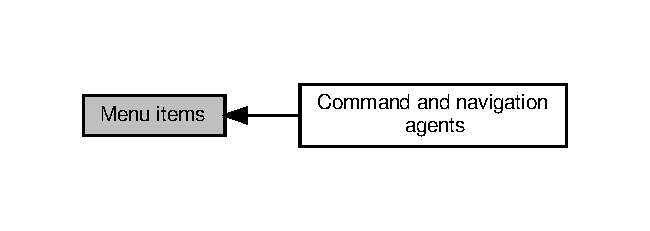
\includegraphics[width=312pt]{group__Items}
\end{center}
\end{figure}
\subsection*{Modules}
\begin{DoxyCompactItemize}
\item 
\hyperlink{group__Agents}{Command and navigation agents}
\end{DoxyCompactItemize}
\subsection*{Classes}
\begin{DoxyCompactItemize}
\item 
struct \hyperlink{structItem}{Item}
\item 
struct \hyperlink{structEmpty}{Empty$<$ I $>$}
\item 
struct \hyperlink{structStaticText}{Static\+Text$<$ text, I $>$}
\item 
class \hyperlink{classStaticMenu}{Static\+Menu$<$ I, I\+I $>$}
\item 
struct \hyperlink{structStaticMenu_3_01I_01_4}{Static\+Menu$<$ I $>$}
\item 
struct \hyperlink{structPrompt}{Prompt$<$ I $>$}
\end{DoxyCompactItemize}


\subsection{Detailed Description}

\hypertarget{group__Agents}{}\section{Command and navigation agents}
\label{group__Agents}\index{Command and navigation agents@{Command and navigation agents}}
Collaboration diagram for Command and navigation agents\+:\nopagebreak
\begin{figure}[H]
\begin{center}
\leavevmode
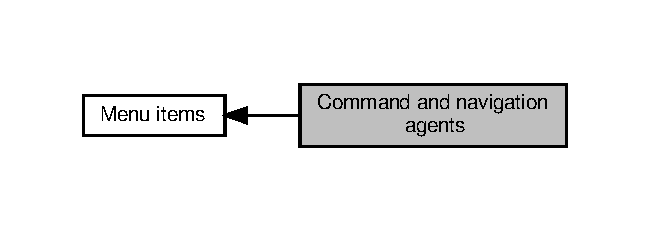
\includegraphics[width=312pt]{group__Agents}
\end{center}
\end{figure}
\subsection*{Classes}
\begin{DoxyCompactItemize}
\item 
struct \hyperlink{structCmdAgent}{Cmd\+Agent}
\item 
struct \hyperlink{structEmptyCmds}{Empty\+Cmds$<$ res $>$}
\item 
struct \hyperlink{structItemCmd}{Item\+Cmd$<$ I, res $>$}
\item 
struct \hyperlink{structNavAgent}{Nav\+Agent}
\item 
class \hyperlink{classNavHandler}{Nav\+Handler$<$ I $>$}
\item 
class \hyperlink{classAction}{Action$<$ I, act $>$}
\end{DoxyCompactItemize}
\subsection*{Typedefs}
\begin{DoxyCompactItemize}
\item 
\mbox{\Hypertarget{group__Agents_gafbac13c24bfb11651f031fcd34ead566}\label{group__Agents_gafbac13c24bfb11651f031fcd34ead566}} 
using \hyperlink{group__Agents_gafbac13c24bfb11651f031fcd34ead566}{Action\+Handler} = bool($\ast$)()
\begin{DoxyCompactList}\small\item\em Action\+Hanlder, type of action functions to associate with items. \end{DoxyCompactList}\end{DoxyCompactItemize}
\subsection*{Functions}
\begin{DoxyCompactItemize}
\item 
bool \hyperlink{group__Agents_ga34d052b903454a7ceda33b9506513683}{do\+Nothing} ()
\begin{DoxyCompactList}\small\item\em means the item has no associated action \end{DoxyCompactList}\item 
static \hyperlink{structNavAgent}{Nav\+Agent} \hyperlink{group__Agents_gade3cccf531dad6fe907c3a9764204e1c}{Empty$<$ I $>$\+::activate} ()
\begin{DoxyCompactList}\small\item\em activate this item (handle enter/select) \end{DoxyCompactList}\end{DoxyCompactItemize}


\subsection{Detailed Description}


\subsection{Function Documentation}
\mbox{\Hypertarget{group__Agents_gade3cccf531dad6fe907c3a9764204e1c}\label{group__Agents_gade3cccf531dad6fe907c3a9764204e1c}} 
\index{Command and navigation agents@{Command and navigation agents}!activate@{activate}}
\index{activate@{activate}!Command and navigation agents@{Command and navigation agents}}
\subsubsection{\texorpdfstring{activate()}{activate()}}
{\footnotesize\ttfamily template$<$typename I $>$ \\
\hyperlink{structNavAgent}{Nav\+Agent} \hyperlink{structEmpty}{Empty}$<$ I $>$\+::activate (\begin{DoxyParamCaption}{ }\end{DoxyParamCaption})\hspace{0.3cm}{\ttfamily [inline]}, {\ttfamily [static]}}



activate this item (handle enter/select) 

activate collection item (handle enter/select) returns a dumb agent to be used by navigation \mbox{\Hypertarget{group__Agents_ga34d052b903454a7ceda33b9506513683}\label{group__Agents_ga34d052b903454a7ceda33b9506513683}} 
\index{Command and navigation agents@{Command and navigation agents}!do\+Nothing@{do\+Nothing}}
\index{do\+Nothing@{do\+Nothing}!Command and navigation agents@{Command and navigation agents}}
\subsubsection{\texorpdfstring{do\+Nothing()}{doNothing()}}
{\footnotesize\ttfamily bool do\+Nothing (\begin{DoxyParamCaption}{ }\end{DoxyParamCaption})\hspace{0.3cm}{\ttfamily [inline]}}



means the item has no associated action 

\begin{DoxyReturn}{Returns}
always false, the item will not handle navigation
\end{DoxyReturn}
this is a comodity 
\hypertarget{group__Navigation}{}\section{Navigation system}
\label{group__Navigation}\index{Navigation system@{Navigation system}}
\subsection*{Classes}
\begin{DoxyCompactItemize}
\item 
struct \hyperlink{structDrift}{Drift$<$ N $>$}
\item 
class \hyperlink{classNavBase}{Nav\+Base$<$ Out, N $>$}
\item 
class \hyperlink{classStaticNav}{Static\+Nav$<$ Out, Data, N $>$}
\item 
class \hyperlink{classDynamicNav}{Dynamic\+Nav$<$ Out, Data, N $>$}
\item 
class \hyperlink{classNavPos}{Nav\+Pos$<$ N $>$}
\item 
class \hyperlink{classItemNav}{Item\+Nav$<$ N $>$}
\item 
struct \hyperlink{structNavCap}{Nav\+Cap$<$ N $>$}
\end{DoxyCompactItemize}


\subsection{Detailed Description}

\hypertarget{group__Output}{}\section{Menu output}
\label{group__Output}\index{Menu output@{Menu output}}
\subsection*{Classes}
\begin{DoxyCompactItemize}
\item 
struct \hyperlink{structRawOut}{Raw\+Out$<$ Dev, dev, O $>$}
\item 
struct \hyperlink{structMenuOutDef}{Menu\+Out\+Def$<$ O $>$}
\end{DoxyCompactItemize}


\subsection{Detailed Description}

\hypertarget{group__Printers}{}\section{Part printing}
\label{group__Printers}\index{Part printing@{Part printing}}
\subsection*{Classes}
\begin{DoxyCompactItemize}
\item 
struct \hyperlink{structFullPrinter}{Full\+Printer$<$ P $>$}
\end{DoxyCompactItemize}


\subsection{Detailed Description}

\chapter{Class Documentation}
\hypertarget{classAction}{}\section{Action$<$ I, act $>$ Class Template Reference}
\label{classAction}\index{Action$<$ I, act $>$@{Action$<$ I, act $>$}}


{\ttfamily \#include $<$item.\+h$>$}



Inheritance diagram for Action$<$ I, act $>$\+:\nopagebreak
\begin{figure}[H]
\begin{center}
\leavevmode
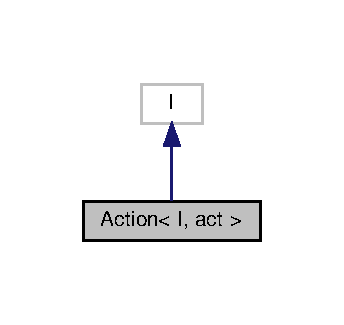
\includegraphics[width=165pt]{classAction__inherit__graph}
\end{center}
\end{figure}


Collaboration diagram for Action$<$ I, act $>$\+:\nopagebreak
\begin{figure}[H]
\begin{center}
\leavevmode
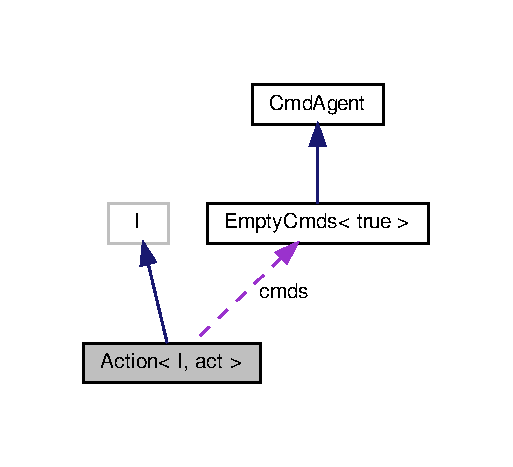
\includegraphics[width=246pt]{classAction__coll__graph}
\end{center}
\end{figure}
\subsection*{Public Types}
\begin{DoxyCompactItemize}
\item 
\mbox{\Hypertarget{classAction_a3a2c0d6cb66ded45aad64c9a1d82fd90}\label{classAction_a3a2c0d6cb66ded45aad64c9a1d82fd90}} 
using {\bfseries This} = \hyperlink{classAction}{Action}$<$ I, act $>$
\end{DoxyCompactItemize}
\subsection*{Public Member Functions}
\begin{DoxyCompactItemize}
\item 
\mbox{\Hypertarget{classAction_a1a642e0df4201fa781e8143da61fd808}\label{classAction_a1a642e0df4201fa781e8143da61fd808}} 
\hyperlink{structNavAgent}{Nav\+Agent} {\bfseries activate} ()
\end{DoxyCompactItemize}
\subsection*{Static Protected Attributes}
\begin{DoxyCompactItemize}
\item 
\mbox{\Hypertarget{classAction_a57b5b2e5b0668ae93053afc3a48ebc81}\label{classAction_a57b5b2e5b0668ae93053afc3a48ebc81}} 
static \hyperlink{structEmptyCmds}{Empty\+Cmds}$<$ true $>$ {\bfseries cmds}
\end{DoxyCompactItemize}


\subsection{Detailed Description}
\subsubsection*{template$<$typename I, Action\+Handler act = do\+Nothing$>$\newline
class Action$<$ I, act $>$}

The \hyperlink{classAction}{Action} class associates an actikon function with a menu item. 

The documentation for this class was generated from the following files\+:\begin{DoxyCompactItemize}
\item 
src/menu/\hyperlink{item_8h}{item.\+h}\item 
src/menu/item.\+hpp\end{DoxyCompactItemize}

\hypertarget{structAsMode}{}\section{As\+Mode$<$ I $>$ Struct Template Reference}
\label{structAsMode}\index{As\+Mode$<$ I $>$@{As\+Mode$<$ I $>$}}


Inheritance diagram for As\+Mode$<$ I $>$\+:
\nopagebreak
\begin{figure}[H]
\begin{center}
\leavevmode
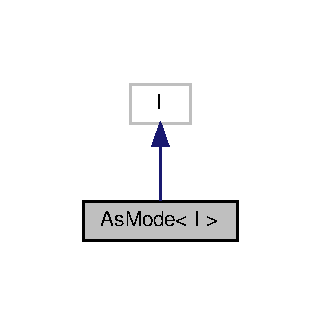
\includegraphics[width=154pt]{structAsMode__inherit__graph}
\end{center}
\end{figure}


Collaboration diagram for As\+Mode$<$ I $>$\+:
\nopagebreak
\begin{figure}[H]
\begin{center}
\leavevmode
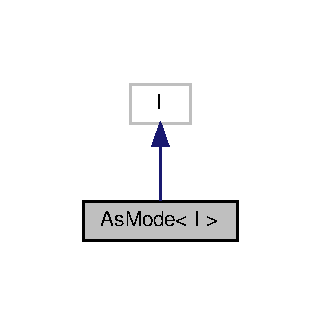
\includegraphics[width=154pt]{structAsMode__coll__graph}
\end{center}
\end{figure}
\subsection*{Public Types}
\begin{DoxyCompactItemize}
\item 
\mbox{\Hypertarget{structAsMode_a40b38b801c92c71f62669fd54a733fc1}\label{structAsMode_a40b38b801c92c71f62669fd54a733fc1}} 
using {\bfseries This} = \hyperlink{structAsMode}{As\+Mode}$<$ I $>$
\end{DoxyCompactItemize}
\subsection*{Public Member Functions}
\begin{DoxyCompactItemize}
\item 
\mbox{\Hypertarget{structAsMode_a9960667927b41780bf7d9e4aa8bac7bf}\label{structAsMode_a9960667927b41780bf7d9e4aa8bac7bf}} 
{\footnotesize template$<$typename Nav , typename Out $>$ }\\void {\bfseries print} (Nav \&nav, Out \&out)
\end{DoxyCompactItemize}


The documentation for this struct was generated from the following file\+:\begin{DoxyCompactItemize}
\item 
src/menu/\hyperlink{item_8h}{item.\+h}\end{DoxyCompactItemize}

\hypertarget{structAsUnit}{}\section{As\+Unit$<$ I $>$ Struct Template Reference}
\label{structAsUnit}\index{As\+Unit$<$ I $>$@{As\+Unit$<$ I $>$}}


{\ttfamily \#include $<$item.\+h$>$}



Inheritance diagram for As\+Unit$<$ I $>$\+:\nopagebreak
\begin{figure}[H]
\begin{center}
\leavevmode
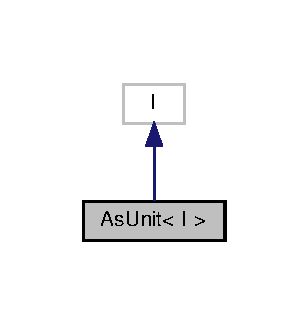
\includegraphics[width=148pt]{structAsUnit__inherit__graph}
\end{center}
\end{figure}


Collaboration diagram for As\+Unit$<$ I $>$\+:\nopagebreak
\begin{figure}[H]
\begin{center}
\leavevmode
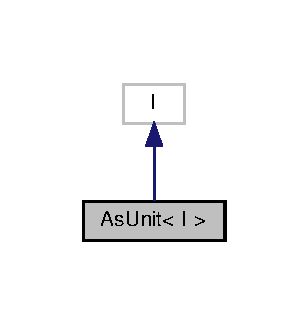
\includegraphics[width=148pt]{structAsUnit__coll__graph}
\end{center}
\end{figure}
\subsection*{Public Types}
\begin{DoxyCompactItemize}
\item 
\mbox{\Hypertarget{structAsUnit_a025932fdf9b0f80c22edfd96d9cc28a5}\label{structAsUnit_a025932fdf9b0f80c22edfd96d9cc28a5}} 
using {\bfseries This} = \hyperlink{structAsUnit}{As\+Unit}$<$ I $>$
\end{DoxyCompactItemize}
\subsection*{Public Member Functions}
\begin{DoxyCompactItemize}
\item 
\mbox{\Hypertarget{structAsUnit_a616d2dd2d3909db6766e676d04f9ede4}\label{structAsUnit_a616d2dd2d3909db6766e676d04f9ede4}} 
{\footnotesize template$<$typename Nav , typename Out $>$ }\\void {\bfseries print} (Nav \&nav, Out \&out)
\end{DoxyCompactItemize}


\subsection{Detailed Description}
\subsubsection*{template$<$typename I$>$\newline
struct As\+Unit$<$ I $>$}

The \hyperlink{structAsUnit}{As\+Unit} class signals the format system to handle inner content as an unit (normaly append text after a value) 

The documentation for this struct was generated from the following file\+:\begin{DoxyCompactItemize}
\item 
src/menu/\hyperlink{item_8h}{item.\+h}\end{DoxyCompactItemize}

\hypertarget{structAsValue}{}\section{As\+Value$<$ I $>$ Struct Template Reference}
\label{structAsValue}\index{As\+Value$<$ I $>$@{As\+Value$<$ I $>$}}


Inheritance diagram for As\+Value$<$ I $>$\+:
\nopagebreak
\begin{figure}[H]
\begin{center}
\leavevmode
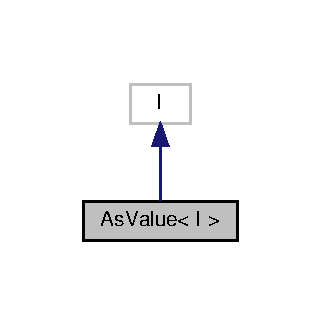
\includegraphics[width=154pt]{structAsValue__inherit__graph}
\end{center}
\end{figure}


Collaboration diagram for As\+Value$<$ I $>$\+:
\nopagebreak
\begin{figure}[H]
\begin{center}
\leavevmode
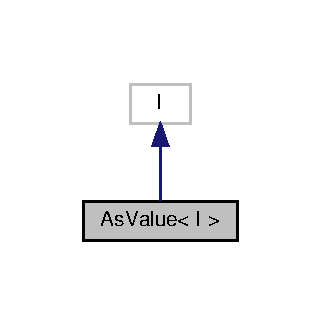
\includegraphics[width=154pt]{structAsValue__coll__graph}
\end{center}
\end{figure}
\subsection*{Public Types}
\begin{DoxyCompactItemize}
\item 
\mbox{\Hypertarget{structAsValue_ac193a16f2751f437dc0a6d2835cb89e5}\label{structAsValue_ac193a16f2751f437dc0a6d2835cb89e5}} 
using {\bfseries This} = \hyperlink{structAsValue}{As\+Value}$<$ I $>$
\end{DoxyCompactItemize}
\subsection*{Public Member Functions}
\begin{DoxyCompactItemize}
\item 
\mbox{\Hypertarget{structAsValue_a4e2ddfac08c8f88bbc93ba4b4e291d6f}\label{structAsValue_a4e2ddfac08c8f88bbc93ba4b4e291d6f}} 
{\footnotesize template$<$typename Nav , typename Out $>$ }\\void {\bfseries print} (Nav \&nav, Out \&out)
\end{DoxyCompactItemize}


The documentation for this struct was generated from the following file\+:\begin{DoxyCompactItemize}
\item 
src/menu/\hyperlink{item_8h}{item.\+h}\end{DoxyCompactItemize}

\hypertarget{structChain}{}\section{Chain$<$ OO $>$ Struct Template Reference}
\label{structChain}\index{Chain$<$ O\+O $>$@{Chain$<$ O\+O $>$}}


{\ttfamily \#include $<$base.\+h$>$}

\subsection*{Classes}
\begin{DoxyCompactItemize}
\item 
struct \hyperlink{structChain_1_1Links}{Links}
\item 
struct \hyperlink{structChain_1_1Links_3_01__T_00_01__O_01_4}{Links$<$ \+\_\+\+T, \+\_\+\+O $>$}
\item 
struct \hyperlink{structChain_1_1To}{To}
\end{DoxyCompactItemize}
\subsection*{Public Types}
\begin{DoxyCompactItemize}
\item 
\mbox{\Hypertarget{structChain_a2a8c5e811335c741b02a946d82a968f8}\label{structChain_a2a8c5e811335c741b02a946d82a968f8}} 
{\footnotesize template$<$Expr \+\_\+O$>$ }\\using {\bfseries With} = \hyperlink{structChain}{Chain}$<$ O\+O..., \+\_\+O $>$
\end{DoxyCompactItemize}


\subsection{Detailed Description}
\subsubsection*{template$<$Expr... OO$>$\newline
struct Chain$<$ O\+O $>$}

The \hyperlink{structChain}{Chain} class is an utility to make composition nesting cleaner and easier to maintain. 

The documentation for this struct was generated from the following file\+:\begin{DoxyCompactItemize}
\item 
src/menu/\hyperlink{base_8h}{base.\+h}\end{DoxyCompactItemize}

\hypertarget{structCmdAgent}{}\section{Cmd\+Agent Struct Reference}
\label{structCmdAgent}\index{Cmd\+Agent@{Cmd\+Agent}}


{\ttfamily \#include $<$item.\+h$>$}



Inheritance diagram for Cmd\+Agent\+:\nopagebreak
\begin{figure}[H]
\begin{center}
\leavevmode
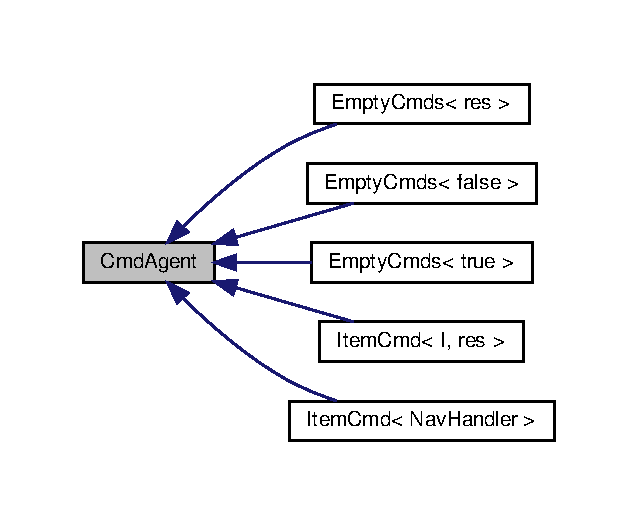
\includegraphics[width=306pt]{structCmdAgent__inherit__graph}
\end{center}
\end{figure}
\subsection*{Public Member Functions}
\begin{DoxyCompactItemize}
\item 
\mbox{\Hypertarget{structCmdAgent_a1a0eedb14708cc96c254922c545915c5}\label{structCmdAgent_a1a0eedb14708cc96c254922c545915c5}} 
virtual bool {\bfseries can\+Nav} () const =0
\item 
\mbox{\Hypertarget{structCmdAgent_a310f823c00f4a7dc427a1d31f6158897}\label{structCmdAgent_a310f823c00f4a7dc427a1d31f6158897}} 
virtual bool {\bfseries up} (void $\ast$o)=0
\item 
\mbox{\Hypertarget{structCmdAgent_ae95a8096248043644ac58cba80a378b2}\label{structCmdAgent_ae95a8096248043644ac58cba80a378b2}} 
virtual bool {\bfseries down} (void $\ast$o)=0
\item 
\mbox{\Hypertarget{structCmdAgent_a673709ce059dbd54d86c61b0fdc9a17a}\label{structCmdAgent_a673709ce059dbd54d86c61b0fdc9a17a}} 
virtual bool {\bfseries enter} (void $\ast$o)=0
\item 
\mbox{\Hypertarget{structCmdAgent_a5fb6b466ecb88ebad13a1e1a1099ef21}\label{structCmdAgent_a5fb6b466ecb88ebad13a1e1a1099ef21}} 
virtual bool {\bfseries esc} (void $\ast$o)=0
\item 
\mbox{\Hypertarget{structCmdAgent_a4836801b65eaf6df12a72ccb8fe0834d}\label{structCmdAgent_a4836801b65eaf6df12a72ccb8fe0834d}} 
virtual bool {\bfseries result} () const =0
\item 
\mbox{\Hypertarget{structCmdAgent_a86f5dd66aade20cb1938669ab52a1311}\label{structCmdAgent_a86f5dd66aade20cb1938669ab52a1311}} 
virtual Modes {\bfseries mode} () const
\end{DoxyCompactItemize}


\subsection{Detailed Description}
The \hyperlink{structCmdAgent}{Cmd\+Agent} class represents an item that might receive navigation commands 

The documentation for this struct was generated from the following file\+:\begin{DoxyCompactItemize}
\item 
src/menu/\hyperlink{item_8h}{item.\+h}\end{DoxyCompactItemize}

\hypertarget{structConsole}{}\section{Console$<$ dev, O $>$ Struct Template Reference}
\label{structConsole}\index{Console$<$ dev, O $>$@{Console$<$ dev, O $>$}}


Inheritance diagram for Console$<$ dev, O $>$\+:\nopagebreak
\begin{figure}[H]
\begin{center}
\leavevmode
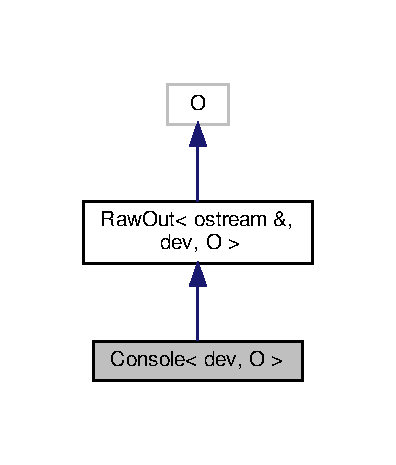
\includegraphics[width=190pt]{structConsole__inherit__graph}
\end{center}
\end{figure}


Collaboration diagram for Console$<$ dev, O $>$\+:\nopagebreak
\begin{figure}[H]
\begin{center}
\leavevmode
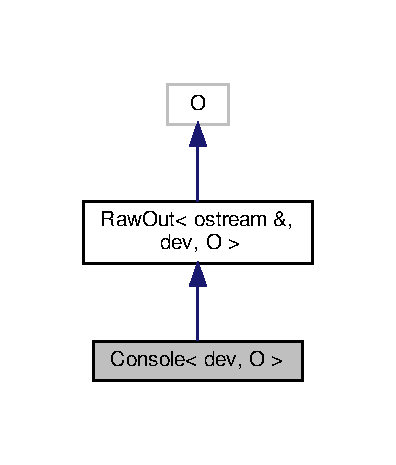
\includegraphics[width=190pt]{structConsole__coll__graph}
\end{center}
\end{figure}
\subsection*{Public Member Functions}
\begin{DoxyCompactItemize}
\item 
\mbox{\Hypertarget{structConsole_ab7a075ab27e0cb666ac5abaaf0c576b1}\label{structConsole_ab7a075ab27e0cb666ac5abaaf0c576b1}} 
{\footnotesize template$<$typename T $>$ }\\void {\bfseries raw} (T i)
\end{DoxyCompactItemize}
\subsection*{Static Public Member Functions}
\begin{DoxyCompactItemize}
\item 
\mbox{\Hypertarget{structConsole_a68249f60fcaaaf8db2b3723ea7252bb1}\label{structConsole_a68249f60fcaaaf8db2b3723ea7252bb1}} 
static void {\bfseries nl} ()
\end{DoxyCompactItemize}


The documentation for this struct was generated from the following file\+:\begin{DoxyCompactItemize}
\item 
src/menu/\+I\+O/\hyperlink{consoleOut_8h}{console\+Out.\+h}\end{DoxyCompactItemize}

\hypertarget{structDrift}{}\section{Drift$<$ O $>$ Struct Template Reference}
\label{structDrift}\index{Drift$<$ O $>$@{Drift$<$ O $>$}}


Inheritance diagram for Drift$<$ O $>$\+:\nopagebreak
\begin{figure}[H]
\begin{center}
\leavevmode
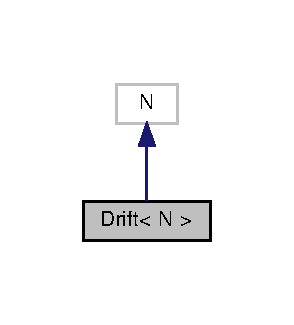
\includegraphics[width=141pt]{structDrift__inherit__graph}
\end{center}
\end{figure}


Collaboration diagram for Drift$<$ O $>$\+:\nopagebreak
\begin{figure}[H]
\begin{center}
\leavevmode
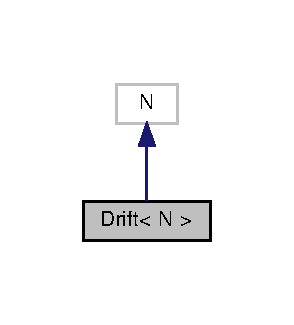
\includegraphics[width=141pt]{structDrift__coll__graph}
\end{center}
\end{figure}
\subsection*{Static Public Member Functions}
\begin{DoxyCompactItemize}
\item 
\mbox{\Hypertarget{structDrift_a9737d0d991f1dba95915858aa43ca356}\label{structDrift_a9737d0d991f1dba95915858aa43ca356}} 
static constexpr bool {\bfseries selected} (idx\+\_\+t)
\item 
\mbox{\Hypertarget{structDrift_ad8fd05fa63905edfe08d9ab678d8dfd3}\label{structDrift_ad8fd05fa63905edfe08d9ab678d8dfd3}} 
static constexpr bool {\bfseries enabled} (idx\+\_\+t)
\item 
\mbox{\Hypertarget{structDrift_abf8c955aef771abbc8e4496998403d3f}\label{structDrift_abf8c955aef771abbc8e4496998403d3f}} 
{\footnotesize template$<$typename Nav $>$ }\\static constexpr bool {\bfseries \+\_\+up} (Nav \&nav)
\item 
\mbox{\Hypertarget{structDrift_a99f89a368f6fb5f5a20cc38ed5894553}\label{structDrift_a99f89a368f6fb5f5a20cc38ed5894553}} 
{\footnotesize template$<$typename Nav $>$ }\\static constexpr bool {\bfseries \+\_\+down} (Nav \&nav)
\item 
\mbox{\Hypertarget{structDrift_ad57b88b6f6900dc584dc8d7f71f50cda}\label{structDrift_ad57b88b6f6900dc584dc8d7f71f50cda}} 
{\footnotesize template$<$typename Nav $>$ }\\static constexpr bool {\bfseries \+\_\+left} (Nav \&nav)
\item 
\mbox{\Hypertarget{structDrift_aa39175b77012010c272db3fba6d635ea}\label{structDrift_aa39175b77012010c272db3fba6d635ea}} 
{\footnotesize template$<$typename Nav $>$ }\\static constexpr bool {\bfseries \+\_\+right} (Nav \&nav)
\item 
\mbox{\Hypertarget{structDrift_a399e70655ae78a3abba826ebcc36f363}\label{structDrift_a399e70655ae78a3abba826ebcc36f363}} 
{\footnotesize template$<$typename Nav $>$ }\\static constexpr bool {\bfseries \+\_\+enter} (Nav \&nav)
\item 
\mbox{\Hypertarget{structDrift_a444d8426671cd25610c2a79799295353}\label{structDrift_a444d8426671cd25610c2a79799295353}} 
{\footnotesize template$<$typename Nav $>$ }\\static constexpr bool {\bfseries \+\_\+esc} (Nav \&nav)
\end{DoxyCompactItemize}


The documentation for this struct was generated from the following file\+:\begin{DoxyCompactItemize}
\item 
src/menu/\hyperlink{nav_8h}{nav.\+h}\end{DoxyCompactItemize}

\hypertarget{classDynamicNav}{}\section{Dynamic\+Nav$<$ Out, Data, N $>$ Class Template Reference}
\label{classDynamicNav}\index{Dynamic\+Nav$<$ Out, Data, N $>$@{Dynamic\+Nav$<$ Out, Data, N $>$}}


{\ttfamily \#include $<$nav.\+h$>$}



Inheritance diagram for Dynamic\+Nav$<$ Out, Data, N $>$\+:\nopagebreak
\begin{figure}[H]
\begin{center}
\leavevmode
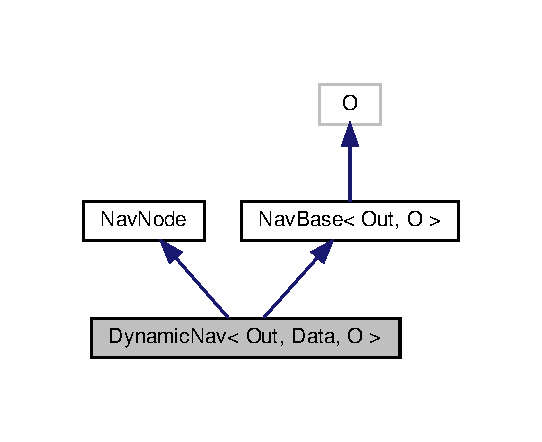
\includegraphics[width=290pt]{classDynamicNav__inherit__graph}
\end{center}
\end{figure}


Collaboration diagram for Dynamic\+Nav$<$ Out, Data, N $>$\+:\nopagebreak
\begin{figure}[H]
\begin{center}
\leavevmode
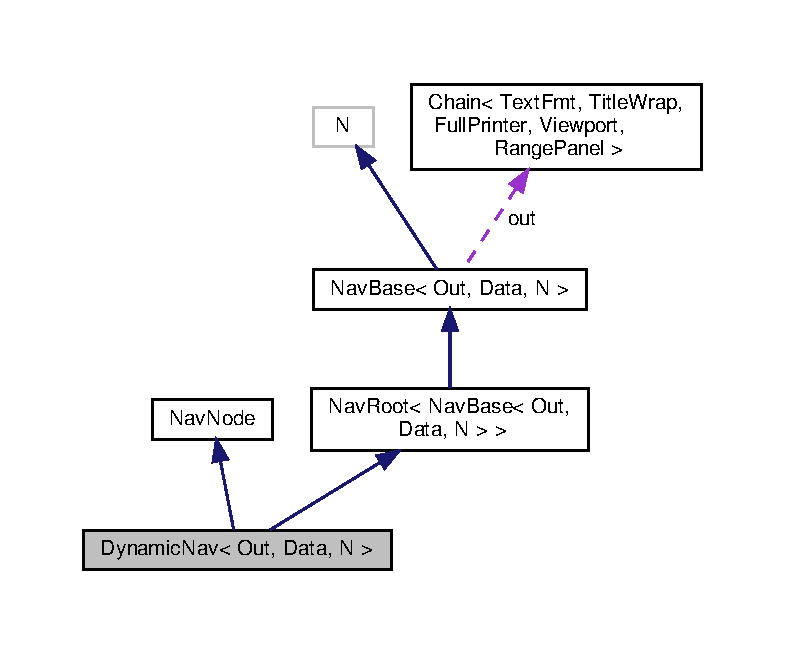
\includegraphics[width=350pt]{classDynamicNav__coll__graph}
\end{center}
\end{figure}
\subsection*{Public Types}
\begin{DoxyCompactItemize}
\item 
\mbox{\Hypertarget{classDynamicNav_a07643e4956c551dd6e73113bb64b907c}\label{classDynamicNav_a07643e4956c551dd6e73113bb64b907c}} 
using {\bfseries Base} = \hyperlink{structNavRoot}{Nav\+Root}$<$ \hyperlink{classNavBase}{Nav\+Base}$<$ Out, Data, N $>$ $>$
\item 
\mbox{\Hypertarget{classDynamicNav_a87dc6c1f5969829af5e073e6d102c443}\label{classDynamicNav_a87dc6c1f5969829af5e073e6d102c443}} 
using {\bfseries This} = \hyperlink{classDynamicNav}{Dynamic\+Nav}$<$ Out, Data, N $>$
\item 
\mbox{\Hypertarget{classDynamicNav_a680da5af4f7c9e2f21222546fa383e79}\label{classDynamicNav_a680da5af4f7c9e2f21222546fa383e79}} 
using {\bfseries Out\+Type} = Out
\item 
\mbox{\Hypertarget{classDynamicNav_a917ade6366ab1535cd2339d69c8a2afa}\label{classDynamicNav_a917ade6366ab1535cd2339d69c8a2afa}} 
using {\bfseries Data\+Type} = Data
\end{DoxyCompactItemize}
\subsection*{Public Member Functions}
\begin{DoxyCompactItemize}
\item 
\mbox{\Hypertarget{classDynamicNav_a25fc31774efe41488da85911226dedba}\label{classDynamicNav_a25fc31774efe41488da85911226dedba}} 
void {\bfseries print\+Menu} ()
\item 
\mbox{\Hypertarget{classDynamicNav_ab83b1dcee3497f8ac1dcf79645d5eda6}\label{classDynamicNav_ab83b1dcee3497f8ac1dcf79645d5eda6}} 
bool {\bfseries selected} (idx\+\_\+t i) const override
\item 
\mbox{\Hypertarget{classDynamicNav_a936bedd336e917789c666b6a8dbda6e2}\label{classDynamicNav_a936bedd336e917789c666b6a8dbda6e2}} 
bool {\bfseries enabled} (idx\+\_\+t i) const override
\item 
\mbox{\Hypertarget{classDynamicNav_a311f6301899fe8022d1188a41b6d3a3d}\label{classDynamicNav_a311f6301899fe8022d1188a41b6d3a3d}} 
bool {\bfseries up} () override
\item 
\mbox{\Hypertarget{classDynamicNav_af29357e2328551fb6d68b5d0652c5cbb}\label{classDynamicNav_af29357e2328551fb6d68b5d0652c5cbb}} 
bool {\bfseries down} () override
\item 
\mbox{\Hypertarget{classDynamicNav_a056c94a768614ce2290ced9030868c75}\label{classDynamicNav_a056c94a768614ce2290ced9030868c75}} 
bool {\bfseries left} () override
\item 
\mbox{\Hypertarget{classDynamicNav_a866d57846795b913329ee39fd670d942}\label{classDynamicNav_a866d57846795b913329ee39fd670d942}} 
bool {\bfseries right} () override
\item 
\mbox{\Hypertarget{classDynamicNav_a1781e521f7d4e267f5e401c6070667b6}\label{classDynamicNav_a1781e521f7d4e267f5e401c6070667b6}} 
bool {\bfseries enter} () override
\item 
\mbox{\Hypertarget{classDynamicNav_abfa730037c5dd6f8902d5f76bba9121b}\label{classDynamicNav_abfa730037c5dd6f8902d5f76bba9121b}} 
bool {\bfseries esc} () override
\end{DoxyCompactItemize}
\subsection*{Additional Inherited Members}


\subsection{Detailed Description}
\subsubsection*{template$<$typename Out, typename Data, typename N = Drift$<$$>$$>$\newline
class Dynamic\+Nav$<$ Out, Data, N $>$}

The \hyperlink{classDynamicNav}{Dynamic\+Nav} class. Can point o other target menu 

The documentation for this class was generated from the following file\+:\begin{DoxyCompactItemize}
\item 
src/menu/\hyperlink{nav_8h}{nav.\+h}\end{DoxyCompactItemize}

\hypertarget{structEmpty}{}\section{Empty$<$ I $>$ Struct Template Reference}
\label{structEmpty}\index{Empty$<$ I $>$@{Empty$<$ I $>$}}


{\ttfamily \#include $<$item.\+h$>$}



Inheritance diagram for Empty$<$ I $>$\+:\nopagebreak
\begin{figure}[H]
\begin{center}
\leavevmode
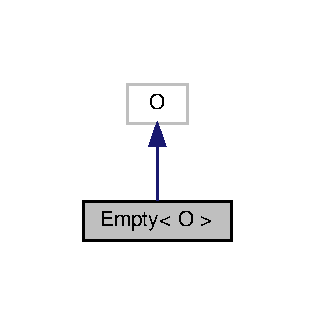
\includegraphics[width=146pt]{structEmpty__inherit__graph}
\end{center}
\end{figure}


Collaboration diagram for Empty$<$ I $>$\+:\nopagebreak
\begin{figure}[H]
\begin{center}
\leavevmode
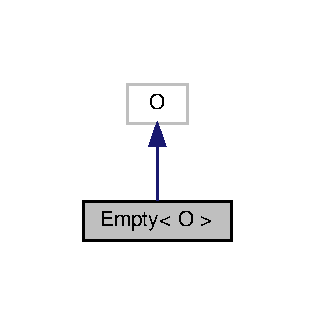
\includegraphics[width=240pt]{structEmpty__coll__graph}
\end{center}
\end{figure}
\subsection*{Public Member Functions}
\begin{DoxyCompactItemize}
\item 
\hyperlink{structItem}{Item} \& \hyperlink{structEmpty_a773bc9093a9594a8227141c9f4f0618f}{operator\mbox{[}$\,$\mbox{]}} (idx\+\_\+t)
\begin{DoxyCompactList}\small\item\em activate this item (handle enter/select) \end{DoxyCompactList}\end{DoxyCompactItemize}
\subsection*{Static Public Member Functions}
\begin{DoxyCompactItemize}
\item 
\mbox{\Hypertarget{structEmpty_afaea8ad71a5e27dbc56c6b6a5a7dc31f}\label{structEmpty_afaea8ad71a5e27dbc56c6b6a5a7dc31f}} 
static constexpr idx\+\_\+t \hyperlink{structEmpty_afaea8ad71a5e27dbc56c6b6a5a7dc31f}{size} ()
\begin{DoxyCompactList}\small\item\em collection size, single elements will return 0 \end{DoxyCompactList}\item 
\mbox{\Hypertarget{structEmpty_ac7dd4689998c86287e66f6184b521ea0}\label{structEmpty_ac7dd4689998c86287e66f6184b521ea0}} 
{\footnotesize template$<$typename Nav , typename Out $>$ }\\static void \hyperlink{structEmpty_ac7dd4689998c86287e66f6184b521ea0}{print} (Nav \&, Out \&)
\begin{DoxyCompactList}\small\item\em print this element to output, some extra info from navigation might be used, such as index \end{DoxyCompactList}\item 
\mbox{\Hypertarget{structEmpty_a7fb2720be72c6c1ab282eb6546b89aad}\label{structEmpty_a7fb2720be72c6c1ab282eb6546b89aad}} 
{\footnotesize template$<$typename Nav , typename Out $>$ }\\static void \hyperlink{structEmpty_a7fb2720be72c6c1ab282eb6546b89aad}{print\+Item} (Nav \&nav, Out \&out, idx\+\_\+t)
\begin{DoxyCompactList}\small\item\em print an item from the collection \end{DoxyCompactList}\item 
\mbox{\Hypertarget{structEmpty_a4a4a935a0441e462d0d8814108bdad22}\label{structEmpty_a4a4a935a0441e462d0d8814108bdad22}} 
static constexpr bool \hyperlink{structEmpty_a4a4a935a0441e462d0d8814108bdad22}{enabled} ()
\begin{DoxyCompactList}\small\item\em is this item enabled? \end{DoxyCompactList}\item 
\mbox{\Hypertarget{structEmpty_adc2d105531fb7b43f60fcd9deaaaa71c}\label{structEmpty_adc2d105531fb7b43f60fcd9deaaaa71c}} 
static constexpr bool \hyperlink{structEmpty_adc2d105531fb7b43f60fcd9deaaaa71c}{enabled} (idx\+\_\+t)
\begin{DoxyCompactList}\small\item\em get enabled status of collection indexed item \end{DoxyCompactList}\item 
\mbox{\Hypertarget{structEmpty_af4997efbad97edae86108c77b4b0f26a}\label{structEmpty_af4997efbad97edae86108c77b4b0f26a}} 
static void \hyperlink{structEmpty_af4997efbad97edae86108c77b4b0f26a}{enable} (idx\+\_\+t, bool)
\begin{DoxyCompactList}\small\item\em set enabled status of indexed collection member \end{DoxyCompactList}\item 
\mbox{\Hypertarget{structEmpty_ade3cccf531dad6fe907c3a9764204e1c}\label{structEmpty_ade3cccf531dad6fe907c3a9764204e1c}} 
static \hyperlink{structNavAgent}{Nav\+Agent} \hyperlink{structEmpty_ade3cccf531dad6fe907c3a9764204e1c}{activate} ()
\begin{DoxyCompactList}\small\item\em returns a dumb agent to be used by navigation \end{DoxyCompactList}\item 
\mbox{\Hypertarget{structEmpty_a2f4d5ca0c3193ed070ef49c4dcc9eb5c}\label{structEmpty_a2f4d5ca0c3193ed070ef49c4dcc9eb5c}} 
static \hyperlink{structNavAgent}{Nav\+Agent} \hyperlink{structEmpty_a2f4d5ca0c3193ed070ef49c4dcc9eb5c}{activate\+Item} (idx\+\_\+t)
\begin{DoxyCompactList}\small\item\em activate collection item by index \end{DoxyCompactList}\item 
\mbox{\Hypertarget{structEmpty_a8b3d397b1910943820e6bf56c3a6bf5d}\label{structEmpty_a8b3d397b1910943820e6bf56c3a6bf5d}} 
static constexpr Modes {\bfseries mode} ()
\item 
\mbox{\Hypertarget{structEmpty_a5d08fca8ef6cedbd25eb086222e8216d}\label{structEmpty_a5d08fca8ef6cedbd25eb086222e8216d}} 
static constexpr bool {\bfseries parent\+Draw} ()
\item 
\mbox{\Hypertarget{structEmpty_ac8835019af0108474e5efe926c008d71}\label{structEmpty_ac8835019af0108474e5efe926c008d71}} 
static constexpr bool {\bfseries is\+Node} ()
\end{DoxyCompactItemize}
\subsection*{Static Public Attributes}
\begin{DoxyCompactItemize}
\item 
\mbox{\Hypertarget{structEmpty_a17b77b2cc02c543127f2db455344f2d3}\label{structEmpty_a17b77b2cc02c543127f2db455344f2d3}} 
static \hyperlink{structEmptyCmds}{Empty\+Cmds}$<$ false $>$ \hyperlink{structEmpty_a17b77b2cc02c543127f2db455344f2d3}{cmds}
\begin{DoxyCompactList}\small\item\em the dumb navigation agent, meaning this item does not handle navigation \end{DoxyCompactList}\end{DoxyCompactItemize}


\subsection{Detailed Description}
\subsubsection*{template$<$typename I = Nil$>$\newline
struct Empty$<$ I $>$}

The \hyperlink{structEmpty}{Empty} class is the static base for menu item elements. It provides minimalist or inexistent implementations. 

\subsection{Member Function Documentation}
\mbox{\Hypertarget{structEmpty_a773bc9093a9594a8227141c9f4f0618f}\label{structEmpty_a773bc9093a9594a8227141c9f4f0618f}} 
\index{Empty@{Empty}!operator\mbox{[}\mbox{]}@{operator[]}}
\index{operator\mbox{[}\mbox{]}@{operator[]}!Empty@{Empty}}
\subsubsection{\texorpdfstring{operator[]()}{operator[]()}}
{\footnotesize\ttfamily template$<$typename I  = Nil$>$ \\
\hyperlink{structItem}{Item}\& \hyperlink{structEmpty}{Empty}$<$ I $>$\+::operator\mbox{[}$\,$\mbox{]} (\begin{DoxyParamCaption}\item[{idx\+\_\+t}]{ }\end{DoxyParamCaption})\hspace{0.3cm}{\ttfamily [inline]}}



activate this item (handle enter/select) 

activate collection item (handle enter/select) 

The documentation for this struct was generated from the following files\+:\begin{DoxyCompactItemize}
\item 
src/menu/\hyperlink{item_8h}{item.\+h}\item 
src/menu/item.\+hpp\end{DoxyCompactItemize}

\hypertarget{structEmptyCmds}{}\section{Empty\+Cmds$<$ res $>$ Struct Template Reference}
\label{structEmptyCmds}\index{Empty\+Cmds$<$ res $>$@{Empty\+Cmds$<$ res $>$}}


{\ttfamily \#include $<$item.\+h$>$}



Inheritance diagram for Empty\+Cmds$<$ res $>$\+:\nopagebreak
\begin{figure}[H]
\begin{center}
\leavevmode
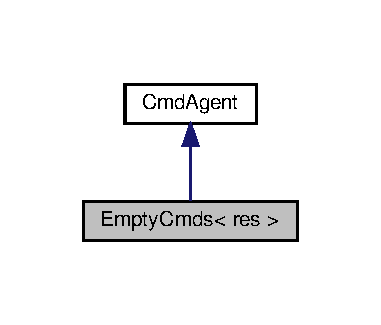
\includegraphics[width=183pt]{structEmptyCmds__inherit__graph}
\end{center}
\end{figure}


Collaboration diagram for Empty\+Cmds$<$ res $>$\+:\nopagebreak
\begin{figure}[H]
\begin{center}
\leavevmode
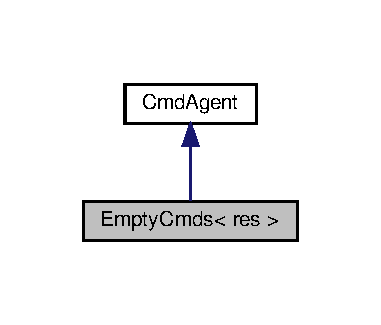
\includegraphics[width=183pt]{structEmptyCmds__coll__graph}
\end{center}
\end{figure}
\subsection*{Public Member Functions}
\begin{DoxyCompactItemize}
\item 
\mbox{\Hypertarget{structEmptyCmds_a0c3644ab3bce97618cf62eb269fdde6d}\label{structEmptyCmds_a0c3644ab3bce97618cf62eb269fdde6d}} 
bool {\bfseries can\+Nav} () const override
\item 
\mbox{\Hypertarget{structEmptyCmds_abcccf9ad7e43d948655938c44b486fa4}\label{structEmptyCmds_abcccf9ad7e43d948655938c44b486fa4}} 
bool {\bfseries result} () const override
\item 
\mbox{\Hypertarget{structEmptyCmds_a3769acda346c1b467fbb6e37b80a5ba4}\label{structEmptyCmds_a3769acda346c1b467fbb6e37b80a5ba4}} 
bool {\bfseries up} (void $\ast$o) override
\item 
\mbox{\Hypertarget{structEmptyCmds_aae723180d4a49785ad9ad1c3ea644b77}\label{structEmptyCmds_aae723180d4a49785ad9ad1c3ea644b77}} 
bool {\bfseries down} (void $\ast$o) override
\item 
\mbox{\Hypertarget{structEmptyCmds_ac79a9fecb8905fbd187c38123f76e64f}\label{structEmptyCmds_ac79a9fecb8905fbd187c38123f76e64f}} 
bool {\bfseries enter} (void $\ast$o) override
\item 
\mbox{\Hypertarget{structEmptyCmds_a6c8bf3dc7a1033fdfe06d79c285f0bd0}\label{structEmptyCmds_a6c8bf3dc7a1033fdfe06d79c285f0bd0}} 
bool {\bfseries esc} (void $\ast$o) override
\end{DoxyCompactItemize}


\subsection{Detailed Description}
\subsubsection*{template$<$bool res = false$>$\newline
struct Empty\+Cmds$<$ res $>$}

The \hyperlink{structEmptyCmds}{Empty\+Cmds} is for items that do not handle nav cmds they can however react to activation and return a true or false version 

The documentation for this struct was generated from the following file\+:\begin{DoxyCompactItemize}
\item 
src/menu/\hyperlink{item_8h}{item.\+h}\end{DoxyCompactItemize}

\hypertarget{classEnDis}{}\section{En\+Dis$<$ O $>$ Class Template Reference}
\label{classEnDis}\index{En\+Dis$<$ O $>$@{En\+Dis$<$ O $>$}}


Inheritance diagram for En\+Dis$<$ O $>$\+:\nopagebreak
\begin{figure}[H]
\begin{center}
\leavevmode
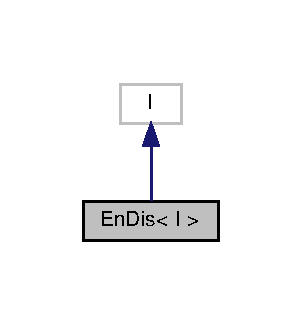
\includegraphics[width=149pt]{classEnDis__inherit__graph}
\end{center}
\end{figure}


Collaboration diagram for En\+Dis$<$ O $>$\+:\nopagebreak
\begin{figure}[H]
\begin{center}
\leavevmode
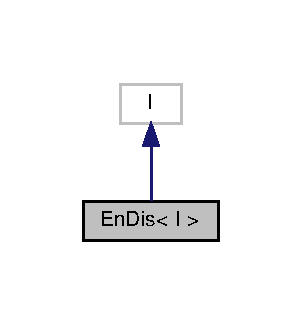
\includegraphics[width=149pt]{classEnDis__coll__graph}
\end{center}
\end{figure}
\subsection*{Public Member Functions}
\begin{DoxyCompactItemize}
\item 
\mbox{\Hypertarget{classEnDis_a8571bb08db08531cd31d6e1051ab484d}\label{classEnDis_a8571bb08db08531cd31d6e1051ab484d}} 
bool {\bfseries enabled} () const
\item 
\mbox{\Hypertarget{classEnDis_a70e85bc35dcc384f0fc1ed456da3ffc0}\label{classEnDis_a70e85bc35dcc384f0fc1ed456da3ffc0}} 
bool {\bfseries enabled} (idx\+\_\+t i) const
\item 
\mbox{\Hypertarget{classEnDis_a8371c78cffd3a88d27acdbd6ba215754}\label{classEnDis_a8371c78cffd3a88d27acdbd6ba215754}} 
void {\bfseries enable} (idx\+\_\+t, bool b)
\end{DoxyCompactItemize}
\subsection*{Protected Attributes}
\begin{DoxyCompactItemize}
\item 
\mbox{\Hypertarget{classEnDis_ae330fda96a39800098254c261b18d889}\label{classEnDis_ae330fda96a39800098254c261b18d889}} 
bool {\bfseries en} =true
\end{DoxyCompactItemize}


The documentation for this class was generated from the following file\+:\begin{DoxyCompactItemize}
\item 
src/menu/comp/\hyperlink{endis_8h}{endis.\+h}\end{DoxyCompactItemize}

\hypertarget{structFlashText}{}\section{Flash\+Text$<$ T, text, O $>$ Struct Template Reference}
\label{structFlashText}\index{Flash\+Text$<$ T, text, O $>$@{Flash\+Text$<$ T, text, O $>$}}


Inheritance diagram for Flash\+Text$<$ T, text, O $>$\+:\nopagebreak
\begin{figure}[H]
\begin{center}
\leavevmode
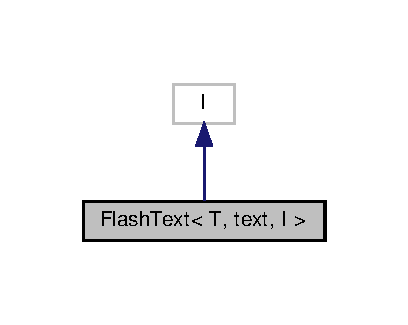
\includegraphics[width=200pt]{structFlashText__inherit__graph}
\end{center}
\end{figure}


Collaboration diagram for Flash\+Text$<$ T, text, O $>$\+:\nopagebreak
\begin{figure}[H]
\begin{center}
\leavevmode
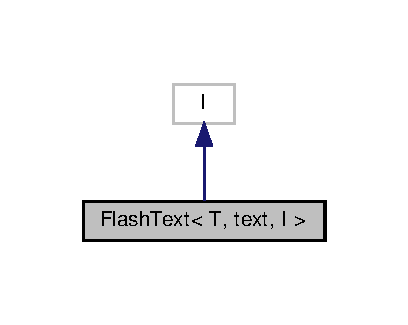
\includegraphics[width=200pt]{structFlashText__coll__graph}
\end{center}
\end{figure}
\subsection*{Public Member Functions}
\begin{DoxyCompactItemize}
\item 
\mbox{\Hypertarget{structFlashText_a8a409170d4bfc09c251ac5aa5760a4d7}\label{structFlashText_a8a409170d4bfc09c251ac5aa5760a4d7}} 
{\footnotesize template$<$typename Nav , typename Out $>$ }\\void {\bfseries print} (Nav \&nav, Out \&out)
\end{DoxyCompactItemize}


The documentation for this struct was generated from the following file\+:\begin{DoxyCompactItemize}
\item 
src/menu/comp/\hyperlink{flashText_8h}{flash\+Text.\+h}\end{DoxyCompactItemize}

\hypertarget{structFullPrinter}{}\section{Full\+Printer$<$ O $>$ Struct Template Reference}
\label{structFullPrinter}\index{Full\+Printer$<$ O $>$@{Full\+Printer$<$ O $>$}}


Inheritance diagram for Full\+Printer$<$ O $>$\+:\nopagebreak
\begin{figure}[H]
\begin{center}
\leavevmode
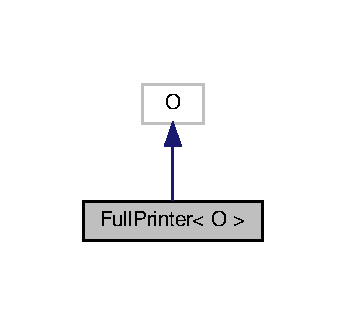
\includegraphics[width=166pt]{structFullPrinter__inherit__graph}
\end{center}
\end{figure}


Collaboration diagram for Full\+Printer$<$ O $>$\+:\nopagebreak
\begin{figure}[H]
\begin{center}
\leavevmode
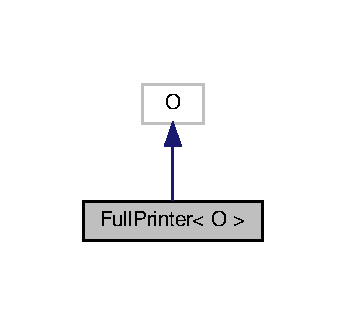
\includegraphics[width=166pt]{structFullPrinter__coll__graph}
\end{center}
\end{figure}
\subsection*{Public Member Functions}
\begin{DoxyCompactItemize}
\item 
\mbox{\Hypertarget{structFullPrinter_af82b8646b09d2ddea62bfa85809f9377}\label{structFullPrinter_af82b8646b09d2ddea62bfa85809f9377}} 
{\footnotesize template$<$typename Nav , typename Out , typename I $>$ }\\void {\bfseries print\+Menu} (Nav \&nav, Out \&out, I \&i)
\end{DoxyCompactItemize}


The documentation for this struct was generated from the following file\+:\begin{DoxyCompactItemize}
\item 
src/menu/\hyperlink{printers_8h}{printers.\+h}\end{DoxyCompactItemize}

\hypertarget{structItem}{}\section{Item Struct Reference}
\label{structItem}\index{Item@{Item}}


Inheritance diagram for Item\+:\nopagebreak
\begin{figure}[H]
\begin{center}
\leavevmode
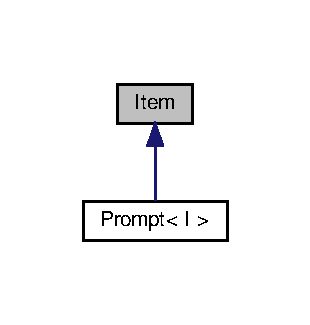
\includegraphics[width=154pt]{structItem__inherit__graph}
\end{center}
\end{figure}
\subsection*{Public Member Functions}
\begin{DoxyCompactItemize}
\item 
\mbox{\Hypertarget{structItem_a48e23000fb91838772b9c9bebbd78497}\label{structItem_a48e23000fb91838772b9c9bebbd78497}} 
virtual void {\bfseries print} (\hyperlink{structNavNode}{Nav\+Node} \&, \hyperlink{structMenuOut}{Menu\+Out} \&out)
\item 
\mbox{\Hypertarget{structItem_a6efc4b4278477e89420279d4cfc480b3}\label{structItem_a6efc4b4278477e89420279d4cfc480b3}} 
virtual void {\bfseries print\+Item} (\hyperlink{structNavNode}{Nav\+Node} \&, \hyperlink{structMenuOut}{Menu\+Out} \&out, idx\+\_\+t n)
\item 
\mbox{\Hypertarget{structItem_a8f540c337986f0ad492f6916c0ed9983}\label{structItem_a8f540c337986f0ad492f6916c0ed9983}} 
virtual void {\bfseries enable} (idx\+\_\+t, bool)
\item 
\mbox{\Hypertarget{structItem_abccd7d2f634cb3c01bdd5941da28d7fc}\label{structItem_abccd7d2f634cb3c01bdd5941da28d7fc}} 
virtual bool {\bfseries enabled} (idx\+\_\+t) const
\item 
\mbox{\Hypertarget{structItem_a27f4a62e0a8c76d3238ddd7c0546de10}\label{structItem_a27f4a62e0a8c76d3238ddd7c0546de10}} 
virtual bool {\bfseries activate} ()
\end{DoxyCompactItemize}


The documentation for this struct was generated from the following file\+:\begin{DoxyCompactItemize}
\item 
src/menu/\hyperlink{base_8h}{base.\+h}\end{DoxyCompactItemize}

\hypertarget{structItemCmd}{}\section{Item\+Cmd$<$ I, res $>$ Struct Template Reference}
\label{structItemCmd}\index{Item\+Cmd$<$ I, res $>$@{Item\+Cmd$<$ I, res $>$}}


{\ttfamily \#include $<$item.\+h$>$}



Inheritance diagram for Item\+Cmd$<$ I, res $>$\+:\nopagebreak
\begin{figure}[H]
\begin{center}
\leavevmode
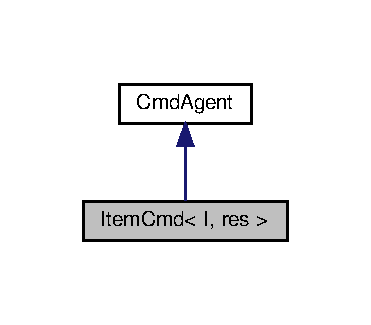
\includegraphics[width=178pt]{structItemCmd__inherit__graph}
\end{center}
\end{figure}


Collaboration diagram for Item\+Cmd$<$ I, res $>$\+:\nopagebreak
\begin{figure}[H]
\begin{center}
\leavevmode
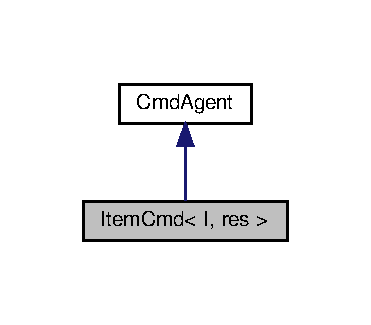
\includegraphics[width=178pt]{structItemCmd__coll__graph}
\end{center}
\end{figure}
\subsection*{Public Member Functions}
\begin{DoxyCompactItemize}
\item 
\mbox{\Hypertarget{structItemCmd_a557f384fe3a5fd259fb780cd625f5999}\label{structItemCmd_a557f384fe3a5fd259fb780cd625f5999}} 
bool {\bfseries can\+Nav} () const override
\item 
\mbox{\Hypertarget{structItemCmd_ad3265b47195a0ef366cceaf9a49006bb}\label{structItemCmd_ad3265b47195a0ef366cceaf9a49006bb}} 
bool {\bfseries result} () const override
\item 
\mbox{\Hypertarget{structItemCmd_a4fdc8aa98593990b0624f23ead5406d5}\label{structItemCmd_a4fdc8aa98593990b0624f23ead5406d5}} 
bool {\bfseries up} (void $\ast$o) override
\item 
\mbox{\Hypertarget{structItemCmd_ac0f94b985d35d18bf876f13bc99b5227}\label{structItemCmd_ac0f94b985d35d18bf876f13bc99b5227}} 
bool {\bfseries down} (void $\ast$o) override
\item 
\mbox{\Hypertarget{structItemCmd_a1fbdc11692ef58433eebfa12b4f102d0}\label{structItemCmd_a1fbdc11692ef58433eebfa12b4f102d0}} 
bool {\bfseries enter} (void $\ast$o) override
\item 
\mbox{\Hypertarget{structItemCmd_a350f85aeabb638c42390f81ffe4a52d6}\label{structItemCmd_a350f85aeabb638c42390f81ffe4a52d6}} 
bool {\bfseries esc} (void $\ast$o) override
\item 
\mbox{\Hypertarget{structItemCmd_a4545584d71b8fece09fe21313c3562c0}\label{structItemCmd_a4545584d71b8fece09fe21313c3562c0}} 
Modes {\bfseries mode} (void $\ast$o) const override
\end{DoxyCompactItemize}


\subsection{Detailed Description}
\subsubsection*{template$<$typename I, bool res = true$>$\newline
struct Item\+Cmd$<$ I, res $>$}

The \hyperlink{structItemCmd}{Item\+Cmd} class provides access to navigation functions of a specific item system generated this types automatically and maps to object functions 

The documentation for this struct was generated from the following file\+:\begin{DoxyCompactItemize}
\item 
src/menu/\hyperlink{item_8h}{item.\+h}\end{DoxyCompactItemize}

\hypertarget{classItemNav}{}\section{Item\+Nav$<$ N $>$ Class Template Reference}
\label{classItemNav}\index{Item\+Nav$<$ N $>$@{Item\+Nav$<$ N $>$}}


{\ttfamily \#include $<$nav.\+h$>$}



Inheritance diagram for Item\+Nav$<$ N $>$\+:\nopagebreak
\begin{figure}[H]
\begin{center}
\leavevmode
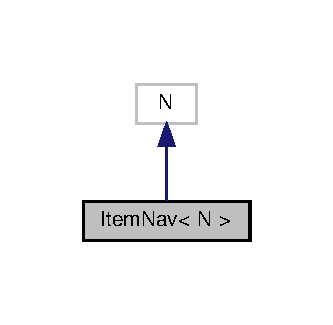
\includegraphics[width=160pt]{classItemNav__inherit__graph}
\end{center}
\end{figure}


Collaboration diagram for Item\+Nav$<$ N $>$\+:\nopagebreak
\begin{figure}[H]
\begin{center}
\leavevmode
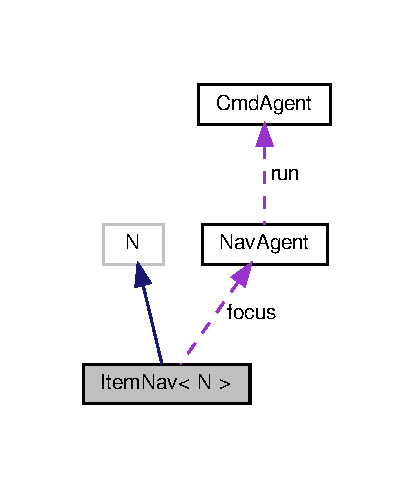
\includegraphics[width=199pt]{classItemNav__coll__graph}
\end{center}
\end{figure}
\subsection*{Public Types}
\begin{DoxyCompactItemize}
\item 
\mbox{\Hypertarget{classItemNav_a6efca103e15edfd3882d78ef119da839}\label{classItemNav_a6efca103e15edfd3882d78ef119da839}} 
using {\bfseries Out\+Type} = typename N\+::\+Out\+Type
\item 
\mbox{\Hypertarget{classItemNav_ad5372e07cabe1fe3f121bd1aa94616ff}\label{classItemNav_ad5372e07cabe1fe3f121bd1aa94616ff}} 
using {\bfseries Data\+Type} = typename N\+::\+Data\+Type
\end{DoxyCompactItemize}
\subsection*{Public Member Functions}
\begin{DoxyCompactItemize}
\item 
\mbox{\Hypertarget{classItemNav_a88d3da019727c248ca83b6a5bd1b6ae3}\label{classItemNav_a88d3da019727c248ca83b6a5bd1b6ae3}} 
{\footnotesize template$<$typename Nav $>$ }\\bool {\bfseries \+\_\+down} (Nav \&nav)
\item 
\mbox{\Hypertarget{classItemNav_a97d9b170b12a5e934233fda1c116b34b}\label{classItemNav_a97d9b170b12a5e934233fda1c116b34b}} 
{\footnotesize template$<$typename Nav $>$ }\\bool {\bfseries \+\_\+up} (Nav \&nav)
\item 
\mbox{\Hypertarget{classItemNav_a35fce8f3e0412ec96715e071000e7959}\label{classItemNav_a35fce8f3e0412ec96715e071000e7959}} 
{\footnotesize template$<$typename Nav $>$ }\\bool {\bfseries \+\_\+left} (Nav \&nav)
\item 
\mbox{\Hypertarget{classItemNav_a4c50b94f9483147cab5a8e732b8475c0}\label{classItemNav_a4c50b94f9483147cab5a8e732b8475c0}} 
{\footnotesize template$<$typename Nav $>$ }\\bool {\bfseries \+\_\+right} (Nav \&nav)
\item 
\mbox{\Hypertarget{classItemNav_a73524b209a2442d9921a273ed3718af9}\label{classItemNav_a73524b209a2442d9921a273ed3718af9}} 
{\footnotesize template$<$typename Nav $>$ }\\bool {\bfseries \+\_\+enter} (Nav \&nav)
\item 
\mbox{\Hypertarget{classItemNav_a45181d1d1ccbd98500cb2ac060b11ec2}\label{classItemNav_a45181d1d1ccbd98500cb2ac060b11ec2}} 
{\footnotesize template$<$typename Nav $>$ }\\bool {\bfseries \+\_\+esc} (Nav \&nav)
\item 
\mbox{\Hypertarget{classItemNav_a09e97ff88aaecb6558ebb1c73ca7b087}\label{classItemNav_a09e97ff88aaecb6558ebb1c73ca7b087}} 
{\footnotesize template$<$typename Nav $>$ }\\Modes {\bfseries \+\_\+mode} (Nav \&nav) const
\item 
\mbox{\Hypertarget{classItemNav_a6436da73b229fa1ed0fef06113849489}\label{classItemNav_a6436da73b229fa1ed0fef06113849489}} 
bool {\bfseries has\+Focus} () const
\end{DoxyCompactItemize}
\subsection*{Protected Attributes}
\begin{DoxyCompactItemize}
\item 
\mbox{\Hypertarget{classItemNav_a6b58882d926efce27e342fac54fe853a}\label{classItemNav_a6b58882d926efce27e342fac54fe853a}} 
\hyperlink{structNavAgent}{Nav\+Agent} {\bfseries focus}
\end{DoxyCompactItemize}


\subsection{Detailed Description}
\subsubsection*{template$<$typename N$>$\newline
class Item\+Nav$<$ N $>$}

The \hyperlink{classItemNav}{Item\+Nav} class allow items to handle navigation (needed for fields) items can handle up$\vert$down$\vert$enter$\vert$esc left$\vert$right are a thing of the navigation system that can steal focus from the field, an enter is sent to the field instead, to validate the entry 

The documentation for this class was generated from the following file\+:\begin{DoxyCompactItemize}
\item 
src/menu/\hyperlink{nav_8h}{nav.\+h}\end{DoxyCompactItemize}

\hypertarget{structChain_1_1Links}{}\section{Chain$<$ OO $>$\+:\+:Links$<$ \+\_\+T, \+\_\+O, \+\_\+\+OO $>$ Struct Template Reference}
\label{structChain_1_1Links}\index{Chain$<$ O\+O $>$\+::\+Links$<$ \+\_\+\+T, \+\_\+\+O, \+\_\+\+O\+O $>$@{Chain$<$ O\+O $>$\+::\+Links$<$ \+\_\+\+T, \+\_\+\+O, \+\_\+\+O\+O $>$}}


Inheritance diagram for Chain$<$ OO $>$\+:\+:Links$<$ \+\_\+T, \+\_\+O, \+\_\+\+OO $>$\+:\nopagebreak
\begin{figure}[H]
\begin{center}
\leavevmode
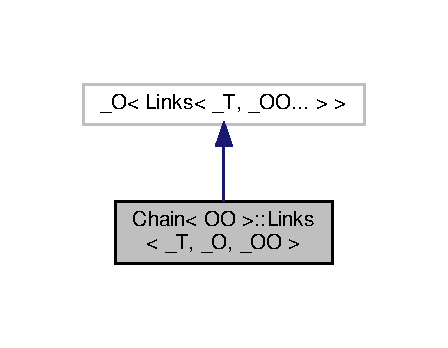
\includegraphics[width=215pt]{structChain_1_1Links__inherit__graph}
\end{center}
\end{figure}


Collaboration diagram for Chain$<$ OO $>$\+:\+:Links$<$ \+\_\+T, \+\_\+O, \+\_\+\+OO $>$\+:\nopagebreak
\begin{figure}[H]
\begin{center}
\leavevmode
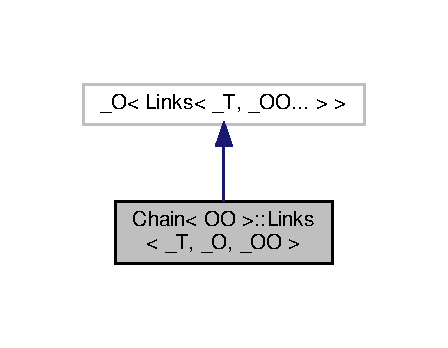
\includegraphics[width=215pt]{structChain_1_1Links__coll__graph}
\end{center}
\end{figure}


The documentation for this struct was generated from the following file\+:\begin{DoxyCompactItemize}
\item 
src/menu/\hyperlink{base_8h}{base.\+h}\end{DoxyCompactItemize}

\hypertarget{structChain_1_1Links_3_01__T_00_01__O_01_4}{}\section{Chain$<$ OO $>$\+:\+:Links$<$ \+\_\+T, \+\_\+O $>$ Struct Template Reference}
\label{structChain_1_1Links_3_01__T_00_01__O_01_4}\index{Chain$<$ O\+O $>$\+::\+Links$<$ \+\_\+\+T, \+\_\+\+O $>$@{Chain$<$ O\+O $>$\+::\+Links$<$ \+\_\+\+T, \+\_\+\+O $>$}}


Inheritance diagram for Chain$<$ OO $>$\+:\+:Links$<$ \+\_\+T, \+\_\+O $>$\+:\nopagebreak
\begin{figure}[H]
\begin{center}
\leavevmode
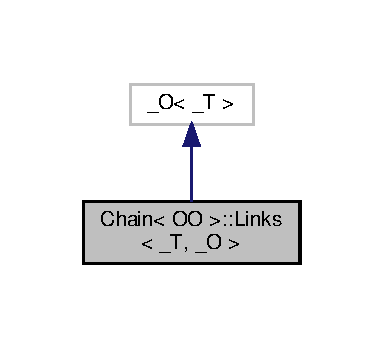
\includegraphics[width=184pt]{structChain_1_1Links_3_01__T_00_01__O_01_4__inherit__graph}
\end{center}
\end{figure}


Collaboration diagram for Chain$<$ OO $>$\+:\+:Links$<$ \+\_\+T, \+\_\+O $>$\+:\nopagebreak
\begin{figure}[H]
\begin{center}
\leavevmode
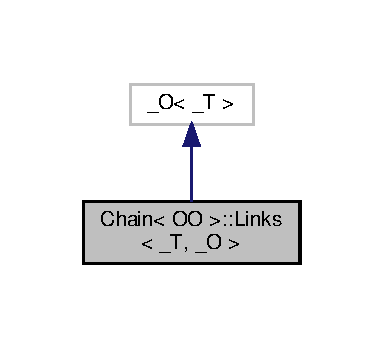
\includegraphics[width=184pt]{structChain_1_1Links_3_01__T_00_01__O_01_4__coll__graph}
\end{center}
\end{figure}


The documentation for this struct was generated from the following file\+:\begin{DoxyCompactItemize}
\item 
src/menu/\hyperlink{base_8h}{base.\+h}\end{DoxyCompactItemize}

\hypertarget{structLiquidCrystalOut}{}\section{Liquid\+Crystal\+Out$<$ dev, O $>$ Struct Template Reference}
\label{structLiquidCrystalOut}\index{Liquid\+Crystal\+Out$<$ dev, O $>$@{Liquid\+Crystal\+Out$<$ dev, O $>$}}


Inheritance diagram for Liquid\+Crystal\+Out$<$ dev, O $>$\+:\nopagebreak
\begin{figure}[H]
\begin{center}
\leavevmode
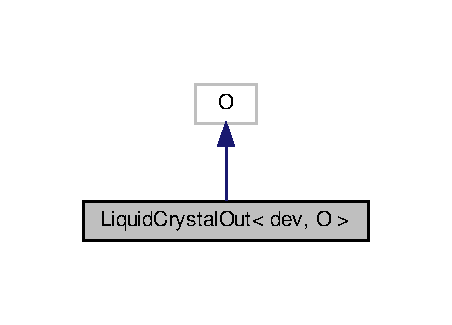
\includegraphics[width=217pt]{structLiquidCrystalOut__inherit__graph}
\end{center}
\end{figure}


Collaboration diagram for Liquid\+Crystal\+Out$<$ dev, O $>$\+:\nopagebreak
\begin{figure}[H]
\begin{center}
\leavevmode
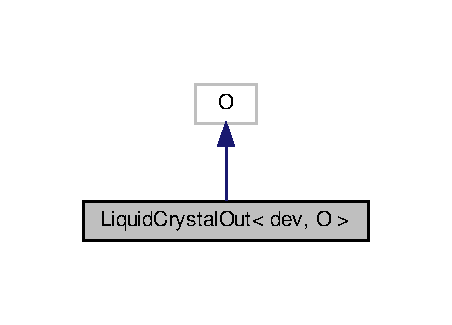
\includegraphics[width=217pt]{structLiquidCrystalOut__coll__graph}
\end{center}
\end{figure}
\subsection*{Public Types}
\begin{DoxyCompactItemize}
\item 
\mbox{\Hypertarget{structLiquidCrystalOut_a26c8d15af8dc0aec9411945fe3725a3d}\label{structLiquidCrystalOut_a26c8d15af8dc0aec9411945fe3725a3d}} 
using {\bfseries This} = \hyperlink{structLiquidCrystalOut}{Liquid\+Crystal\+Out}$<$ dev, O $>$
\end{DoxyCompactItemize}
\subsection*{Public Member Functions}
\begin{DoxyCompactItemize}
\item 
\mbox{\Hypertarget{structLiquidCrystalOut_ad4a4f2eb89f2668019860c3130fd0712}\label{structLiquidCrystalOut_ad4a4f2eb89f2668019860c3130fd0712}} 
{\footnotesize template$<$typename T $>$ }\\void {\bfseries raw} (T i)
\end{DoxyCompactItemize}
\subsection*{Static Public Member Functions}
\begin{DoxyCompactItemize}
\item 
\mbox{\Hypertarget{structLiquidCrystalOut_ae913f308ae361afba546e7f23c2cad55}\label{structLiquidCrystalOut_ae913f308ae361afba546e7f23c2cad55}} 
static void {\bfseries set\+Cursor} (idx\+\_\+t x, idx\+\_\+t y)
\item 
\mbox{\Hypertarget{structLiquidCrystalOut_aedc93cdd2c7a7dcaa98079ad4f4bf584}\label{structLiquidCrystalOut_aedc93cdd2c7a7dcaa98079ad4f4bf584}} 
{\footnotesize template$<$typename Out $>$ }\\static void {\bfseries clr\+Line} (Out \&out, idx\+\_\+t n)
\end{DoxyCompactItemize}


The documentation for this struct was generated from the following file\+:\begin{DoxyCompactItemize}
\item 
src/menu/\+I\+O/\hyperlink{liquidCrystalOut_8h}{liquid\+Crystal\+Out.\+h}\end{DoxyCompactItemize}

\hypertarget{structMenuOut}{}\section{Menu\+Out Struct Reference}
\label{structMenuOut}\index{Menu\+Out@{Menu\+Out}}


Inheritance diagram for Menu\+Out\+:\nopagebreak
\begin{figure}[H]
\begin{center}
\leavevmode
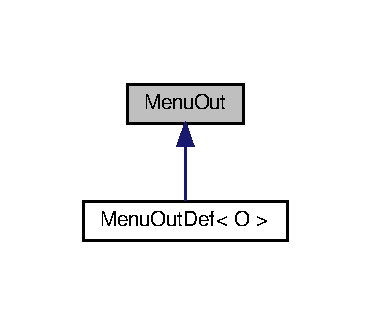
\includegraphics[width=178pt]{structMenuOut__inherit__graph}
\end{center}
\end{figure}
\subsection*{Public Member Functions}
\begin{DoxyCompactItemize}
\item 
\mbox{\Hypertarget{structMenuOut_ad050b1d54cc0ab46ebe877b2d6ff4c31}\label{structMenuOut_ad050b1d54cc0ab46ebe877b2d6ff4c31}} 
virtual void {\bfseries nl} ()
\item 
\mbox{\Hypertarget{structMenuOut_adf86b6ce1d91d71b701cd2651a2d92f5}\label{structMenuOut_adf86b6ce1d91d71b701cd2651a2d92f5}} 
virtual void {\bfseries raw} (char)
\item 
\mbox{\Hypertarget{structMenuOut_a6b833edd18f9ae956fc30b67f34de684}\label{structMenuOut_a6b833edd18f9ae956fc30b67f34de684}} 
virtual void {\bfseries raw} (const char $\ast$)
\item 
\mbox{\Hypertarget{structMenuOut_a675212b21eb703dfabf22c0a92625827}\label{structMenuOut_a675212b21eb703dfabf22c0a92625827}} 
virtual void {\bfseries raw} (int)
\item 
\mbox{\Hypertarget{structMenuOut_a39ff3bae07e2c0d07b5876cbc41d7db7}\label{structMenuOut_a39ff3bae07e2c0d07b5876cbc41d7db7}} 
virtual void {\bfseries raw} (unsigned int)
\item 
\mbox{\Hypertarget{structMenuOut_a0ba6c90717513f82da4d77c5606fcbbb}\label{structMenuOut_a0ba6c90717513f82da4d77c5606fcbbb}} 
virtual void {\bfseries raw} (long)
\item 
\mbox{\Hypertarget{structMenuOut_ad345ce430a5e2e1d02bf1d65ffe120b3}\label{structMenuOut_ad345ce430a5e2e1d02bf1d65ffe120b3}} 
virtual void {\bfseries raw} (unsigned long)
\item 
\mbox{\Hypertarget{structMenuOut_acfa10821cff88f9986d643029516198f}\label{structMenuOut_acfa10821cff88f9986d643029516198f}} 
virtual void {\bfseries raw} (double)
\item 
\mbox{\Hypertarget{structMenuOut_ac1f30c588c0349d9f865f873a09d2268}\label{structMenuOut_ac1f30c588c0349d9f865f873a09d2268}} 
virtual void {\bfseries print\+Item} (\hyperlink{structNavNode}{Nav\+Node} \&, \hyperlink{structItem}{Item} \&, idx\+\_\+t)=0
\item 
\mbox{\Hypertarget{structMenuOut_af40844bea29055ba952fabad9fb22a2c}\label{structMenuOut_af40844bea29055ba952fabad9fb22a2c}} 
virtual void {\bfseries fmt} (Roles role, bool io, \hyperlink{structNavNode}{Nav\+Node} \&nav, \hyperlink{structMenuOut}{Menu\+Out} \&, \hyperlink{structItem}{Item} \&i, idx\+\_\+t)
\item 
\mbox{\Hypertarget{structMenuOut_a088035e2856035a800abccba10a7299d}\label{structMenuOut_a088035e2856035a800abccba10a7299d}} 
void {\bfseries fmt} (Roles role, \hyperlink{structNavNode}{Nav\+Node} \&nav, \hyperlink{structMenuOut}{Menu\+Out} \&out, \hyperlink{structItem}{Item} \&i, idx\+\_\+t n)
\end{DoxyCompactItemize}


The documentation for this struct was generated from the following file\+:\begin{DoxyCompactItemize}
\item 
src/menu/\hyperlink{base_8h}{base.\+h}\end{DoxyCompactItemize}

\hypertarget{structMenuOutDef}{}\section{Menu\+Out\+Def$<$ O $>$ Struct Template Reference}
\label{structMenuOutDef}\index{Menu\+Out\+Def$<$ O $>$@{Menu\+Out\+Def$<$ O $>$}}


Inheritance diagram for Menu\+Out\+Def$<$ O $>$\+:\nopagebreak
\begin{figure}[H]
\begin{center}
\leavevmode
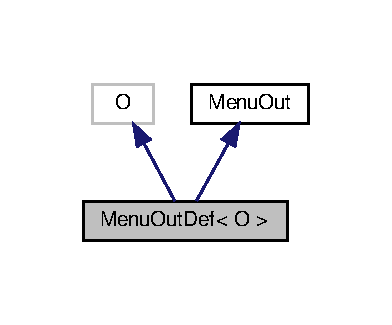
\includegraphics[width=188pt]{structMenuOutDef__inherit__graph}
\end{center}
\end{figure}


Collaboration diagram for Menu\+Out\+Def$<$ O $>$\+:\nopagebreak
\begin{figure}[H]
\begin{center}
\leavevmode
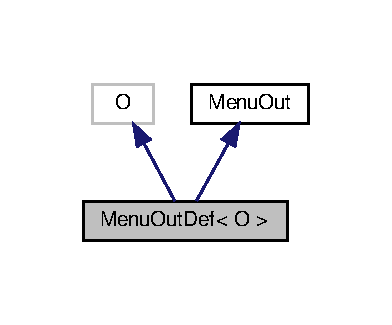
\includegraphics[width=188pt]{structMenuOutDef__coll__graph}
\end{center}
\end{figure}
\subsection*{Public Member Functions}
\begin{DoxyCompactItemize}
\item 
\mbox{\Hypertarget{structMenuOutDef_a3bdf78cf3e8d7d1cfa5ac7259ca7621e}\label{structMenuOutDef_a3bdf78cf3e8d7d1cfa5ac7259ca7621e}} 
void {\bfseries nl} () override
\item 
\mbox{\Hypertarget{structMenuOutDef_a39e40e2057b5826cfb7e7335e34a8ab7}\label{structMenuOutDef_a39e40e2057b5826cfb7e7335e34a8ab7}} 
void {\bfseries raw} (char c) override
\item 
\mbox{\Hypertarget{structMenuOutDef_aa152cf800b2e15afc5ce302578b25e50}\label{structMenuOutDef_aa152cf800b2e15afc5ce302578b25e50}} 
void {\bfseries raw} (const char $\ast$text) override
\item 
\mbox{\Hypertarget{structMenuOutDef_a036d30bc8f65edfd150439f3ecb39494}\label{structMenuOutDef_a036d30bc8f65edfd150439f3ecb39494}} 
void {\bfseries raw} (int n) override
\item 
\mbox{\Hypertarget{structMenuOutDef_a6940e8010dff0dc9b0aee9e899e96168}\label{structMenuOutDef_a6940e8010dff0dc9b0aee9e899e96168}} 
void {\bfseries raw} (unsigned int n) override
\item 
\mbox{\Hypertarget{structMenuOutDef_ad11ac90acb590394dc7adaa96a83ecc0}\label{structMenuOutDef_ad11ac90acb590394dc7adaa96a83ecc0}} 
void {\bfseries raw} (long n) override
\item 
\mbox{\Hypertarget{structMenuOutDef_a956cfa61db20321a27339db830e89001}\label{structMenuOutDef_a956cfa61db20321a27339db830e89001}} 
void {\bfseries raw} (unsigned long n) override
\item 
\mbox{\Hypertarget{structMenuOutDef_a29bfe7f19880b633c76bf75cb43ef786}\label{structMenuOutDef_a29bfe7f19880b633c76bf75cb43ef786}} 
void {\bfseries raw} (double n) override
\item 
\mbox{\Hypertarget{structMenuOutDef_a9f373df24ad0f16625dd1ba97b422491}\label{structMenuOutDef_a9f373df24ad0f16625dd1ba97b422491}} 
void {\bfseries print\+Item} (\hyperlink{structNavNode}{Nav\+Node} \&nav, \hyperlink{structItem}{Item} \&i, idx\+\_\+t n) override
\item 
\mbox{\Hypertarget{structMenuOutDef_afea6ae776b595da4c6b0f17b19807a94}\label{structMenuOutDef_afea6ae776b595da4c6b0f17b19807a94}} 
void {\bfseries fmt} (Roles role, bool io, \hyperlink{structNavNode}{Nav\+Node} \&nav, \hyperlink{structMenuOut}{Menu\+Out} \&out, \hyperlink{structItem}{Item} \&i, idx\+\_\+t n) override
\end{DoxyCompactItemize}


The documentation for this struct was generated from the following file\+:\begin{DoxyCompactItemize}
\item 
src/menu/\hyperlink{out_8h}{out.\+h}\end{DoxyCompactItemize}

\hypertarget{structNavAgent}{}\section{Nav\+Agent Struct Reference}
\label{structNavAgent}\index{Nav\+Agent@{Nav\+Agent}}


{\ttfamily \#include $<$item.\+h$>$}



Collaboration diagram for Nav\+Agent\+:\nopagebreak
\begin{figure}[H]
\begin{center}
\leavevmode
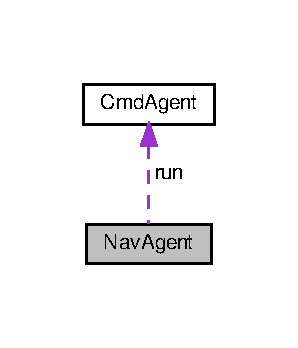
\includegraphics[width=143pt]{structNavAgent__coll__graph}
\end{center}
\end{figure}
\subsection*{Public Member Functions}
\begin{DoxyCompactItemize}
\item 
\mbox{\Hypertarget{structNavAgent_ab1040e3019d1b47d64727a606c41436f}\label{structNavAgent_ab1040e3019d1b47d64727a606c41436f}} 
{\bfseries Nav\+Agent} (void $\ast$o, \hyperlink{structCmdAgent}{Cmd\+Agent} $\ast$r)
\item 
\mbox{\Hypertarget{structNavAgent_a26cd7189c220d855ac814de8d0beaa05}\label{structNavAgent_a26cd7189c220d855ac814de8d0beaa05}} 
{\bfseries Nav\+Agent} (const \hyperlink{structNavAgent}{Nav\+Agent} \&o)
\item 
\mbox{\Hypertarget{structNavAgent_a6daf32fef333fa9a479c51270362ceb7}\label{structNavAgent_a6daf32fef333fa9a479c51270362ceb7}} 
\hyperlink{structNavAgent}{Nav\+Agent} {\bfseries operator=} (\hyperlink{structNavAgent}{Nav\+Agent} \&\&o)
\item 
\mbox{\Hypertarget{structNavAgent_a4b15b07c152a0dc5348c88ca1595c6d5}\label{structNavAgent_a4b15b07c152a0dc5348c88ca1595c6d5}} 
{\bfseries operator bool} () const
\item 
\mbox{\Hypertarget{structNavAgent_a4bab30c7db65ca0023d1cfbda8459fdd}\label{structNavAgent_a4bab30c7db65ca0023d1cfbda8459fdd}} 
bool {\bfseries can\+Nav} () const
\item 
\mbox{\Hypertarget{structNavAgent_ad7922b692ca111e47ca603bd9c578297}\label{structNavAgent_ad7922b692ca111e47ca603bd9c578297}} 
bool {\bfseries up} ()
\item 
\mbox{\Hypertarget{structNavAgent_ab39959e3b1a2b958dfa6a15f6d1ce864}\label{structNavAgent_ab39959e3b1a2b958dfa6a15f6d1ce864}} 
bool {\bfseries down} ()
\item 
\mbox{\Hypertarget{structNavAgent_abbf23487e6d44743f6a16611cc003511}\label{structNavAgent_abbf23487e6d44743f6a16611cc003511}} 
bool {\bfseries enter} ()
\item 
\mbox{\Hypertarget{structNavAgent_a024b5b6266837683569606acd2fab5ed}\label{structNavAgent_a024b5b6266837683569606acd2fab5ed}} 
bool {\bfseries esc} ()
\item 
\mbox{\Hypertarget{structNavAgent_a953668fa3d7517c4fa6c1d54b4d7e551}\label{structNavAgent_a953668fa3d7517c4fa6c1d54b4d7e551}} 
bool {\bfseries result} () const
\item 
\mbox{\Hypertarget{structNavAgent_a574e7ad5bd62ea9a6a5fa1cf722164d5}\label{structNavAgent_a574e7ad5bd62ea9a6a5fa1cf722164d5}} 
Modes {\bfseries mode} () const
\end{DoxyCompactItemize}
\subsection*{Public Attributes}
\begin{DoxyCompactItemize}
\item 
\mbox{\Hypertarget{structNavAgent_a5c9a3c69aa8811b13b8a1baab9e638d6}\label{structNavAgent_a5c9a3c69aa8811b13b8a1baab9e638d6}} 
void $\ast$ {\bfseries obj}
\item 
\mbox{\Hypertarget{structNavAgent_a546c2683e672c82fdb3f9d1a3f444f94}\label{structNavAgent_a546c2683e672c82fdb3f9d1a3f444f94}} 
\hyperlink{structCmdAgent}{Cmd\+Agent} $\ast$ {\bfseries run}
\end{DoxyCompactItemize}


\subsection{Detailed Description}
The \hyperlink{structNavAgent}{Nav\+Agent} class allow navigation system access to specific item navigation functions. 

The documentation for this struct was generated from the following file\+:\begin{DoxyCompactItemize}
\item 
src/menu/\hyperlink{item_8h}{item.\+h}\end{DoxyCompactItemize}

\hypertarget{classNavBase}{}\section{Nav\+Base$<$ Out, O $>$ Class Template Reference}
\label{classNavBase}\index{Nav\+Base$<$ Out, O $>$@{Nav\+Base$<$ Out, O $>$}}


Inheritance diagram for Nav\+Base$<$ Out, O $>$\+:\nopagebreak
\begin{figure}[H]
\begin{center}
\leavevmode
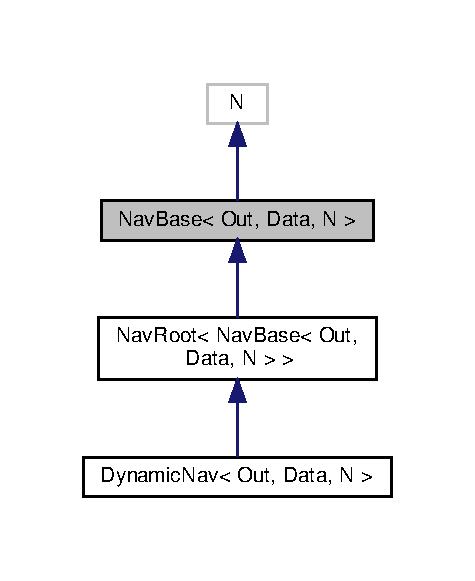
\includegraphics[width=326pt]{classNavBase__inherit__graph}
\end{center}
\end{figure}


Collaboration diagram for Nav\+Base$<$ Out, O $>$\+:\nopagebreak
\begin{figure}[H]
\begin{center}
\leavevmode
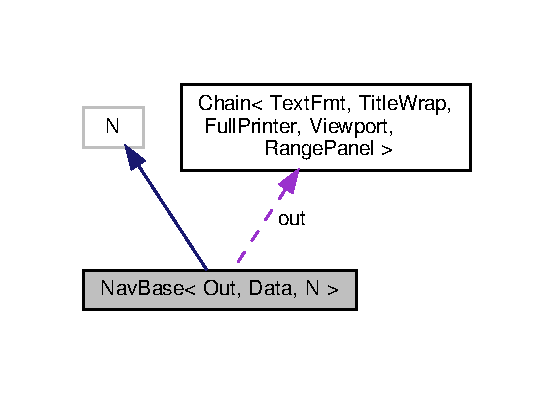
\includegraphics[width=321pt]{classNavBase__coll__graph}
\end{center}
\end{figure}
\subsection*{Public Member Functions}
\begin{DoxyCompactItemize}
\item 
\mbox{\Hypertarget{classNavBase_ad068d1f5452270687488fdf9f545cf0a}\label{classNavBase_ad068d1f5452270687488fdf9f545cf0a}} 
void {\bfseries enter\+Menu\+Render} ()
\item 
\mbox{\Hypertarget{classNavBase_a835de9effe2a6ceeb436bd3d82062702}\label{classNavBase_a835de9effe2a6ceeb436bd3d82062702}} 
void {\bfseries exit\+Menu\+Render} ()
\item 
\mbox{\Hypertarget{classNavBase_a5b46d1597bd8b2f854d32b51eec4a48b}\label{classNavBase_a5b46d1597bd8b2f854d32b51eec4a48b}} 
idx\+\_\+t {\bfseries top} () const
\item 
\mbox{\Hypertarget{classNavBase_a09963109c81e772d2ef3c8cbc3673b9a}\label{classNavBase_a09963109c81e772d2ef3c8cbc3673b9a}} 
void {\bfseries set\+Top} (idx\+\_\+t n)
\item 
\mbox{\Hypertarget{classNavBase_ac978614a7f5571311a306ad60f4f9fd4}\label{classNavBase_ac978614a7f5571311a306ad60f4f9fd4}} 
idx\+\_\+t {\bfseries height} () const
\item 
\mbox{\Hypertarget{classNavBase_a3fc30c3deb16c42b1e77857d255795c7}\label{classNavBase_a3fc30c3deb16c42b1e77857d255795c7}} 
void {\bfseries set\+Focus} (\hyperlink{structItem}{Item} $\ast$i=N\+U\+LL)
\item 
\mbox{\Hypertarget{classNavBase_a2ef0ae3b212cf55b918230dfc1219061}\label{classNavBase_a2ef0ae3b212cf55b918230dfc1219061}} 
void {\bfseries clear\+Focus} ()
\item 
\mbox{\Hypertarget{classNavBase_a32191c597356ae31ad2dda39c0e66e69}\label{classNavBase_a32191c597356ae31ad2dda39c0e66e69}} 
\hyperlink{structItem}{Item} \& {\bfseries get\+Focus} () const
\item 
\mbox{\Hypertarget{classNavBase_aad13dfc1f1b015f0b466ae8d2e7e4098}\label{classNavBase_aad13dfc1f1b015f0b466ae8d2e7e4098}} 
bool {\bfseries has\+Focus} ()
\end{DoxyCompactItemize}
\subsection*{Protected Attributes}
\begin{DoxyCompactItemize}
\item 
\mbox{\Hypertarget{classNavBase_acf44c6a26a5a681ccc3e5799b557ff82}\label{classNavBase_acf44c6a26a5a681ccc3e5799b557ff82}} 
Out {\bfseries out}
\item 
\mbox{\Hypertarget{classNavBase_ab6190d55f74f9f6e8cdd93c9f840df02}\label{classNavBase_ab6190d55f74f9f6e8cdd93c9f840df02}} 
bool {\bfseries on\+Menu} =false
\item 
\mbox{\Hypertarget{classNavBase_a5082aa4acb807202c1e049c16c8e6203}\label{classNavBase_a5082aa4acb807202c1e049c16c8e6203}} 
\hyperlink{structItem}{Item} $\ast$ {\bfseries focus} =N\+U\+LL
\end{DoxyCompactItemize}


The documentation for this class was generated from the following file\+:\begin{DoxyCompactItemize}
\item 
src/menu/\hyperlink{nav_8h}{nav.\+h}\end{DoxyCompactItemize}

\hypertarget{structNavCap}{}\section{Nav\+Cap$<$ O $>$ Struct Template Reference}
\label{structNavCap}\index{Nav\+Cap$<$ O $>$@{Nav\+Cap$<$ O $>$}}


Inheritance diagram for Nav\+Cap$<$ O $>$\+:\nopagebreak
\begin{figure}[H]
\begin{center}
\leavevmode
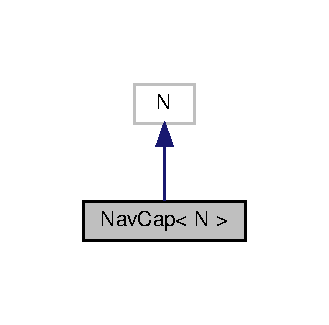
\includegraphics[width=158pt]{structNavCap__inherit__graph}
\end{center}
\end{figure}


Collaboration diagram for Nav\+Cap$<$ O $>$\+:\nopagebreak
\begin{figure}[H]
\begin{center}
\leavevmode
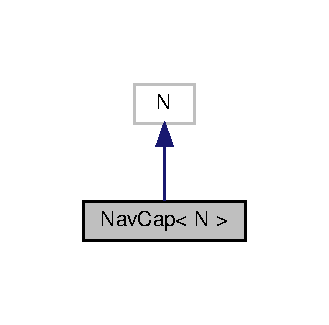
\includegraphics[width=158pt]{structNavCap__coll__graph}
\end{center}
\end{figure}
\subsection*{Public Types}
\begin{DoxyCompactItemize}
\item 
\mbox{\Hypertarget{structNavCap_ae03bc309180ea6ba3c2943b19adf8eb7}\label{structNavCap_ae03bc309180ea6ba3c2943b19adf8eb7}} 
using {\bfseries This} = \hyperlink{structNavCap}{Nav\+Cap}$<$ O $>$
\end{DoxyCompactItemize}
\subsection*{Public Member Functions}
\begin{DoxyCompactItemize}
\item 
\mbox{\Hypertarget{structNavCap_aa0b264a1dcab39a8a3b8d2f9bc814c73}\label{structNavCap_aa0b264a1dcab39a8a3b8d2f9bc814c73}} 
bool {\bfseries up} ()
\item 
\mbox{\Hypertarget{structNavCap_a94f5b1c9871167469e28685c2b6a435f}\label{structNavCap_a94f5b1c9871167469e28685c2b6a435f}} 
bool {\bfseries down} ()
\item 
\mbox{\Hypertarget{structNavCap_a630b475310459b88a75dee9fb07add3c}\label{structNavCap_a630b475310459b88a75dee9fb07add3c}} 
bool {\bfseries left} ()
\item 
\mbox{\Hypertarget{structNavCap_a6e53f7f90c1e3c596383513fa61a0811}\label{structNavCap_a6e53f7f90c1e3c596383513fa61a0811}} 
bool {\bfseries right} ()
\item 
\mbox{\Hypertarget{structNavCap_aa02a28eed35238a9e16d520276df4120}\label{structNavCap_aa02a28eed35238a9e16d520276df4120}} 
bool {\bfseries enter} ()
\item 
\mbox{\Hypertarget{structNavCap_a80a06c48b81a8b181af2eeac311e0304}\label{structNavCap_a80a06c48b81a8b181af2eeac311e0304}} 
bool {\bfseries esc} ()
\end{DoxyCompactItemize}


The documentation for this struct was generated from the following file\+:\begin{DoxyCompactItemize}
\item 
src/menu/\hyperlink{nav_8h}{nav.\+h}\end{DoxyCompactItemize}

\hypertarget{classNavHandler}{}\section{Nav\+Handler$<$ I $>$ Class Template Reference}
\label{classNavHandler}\index{Nav\+Handler$<$ I $>$@{Nav\+Handler$<$ I $>$}}


{\ttfamily \#include $<$item.\+h$>$}



Inheritance diagram for Nav\+Handler$<$ I $>$\+:\nopagebreak
\begin{figure}[H]
\begin{center}
\leavevmode
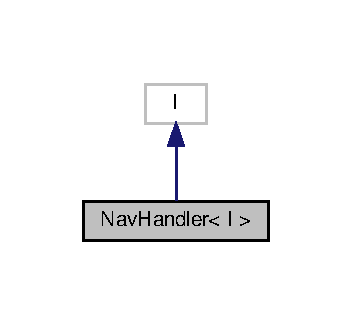
\includegraphics[width=169pt]{classNavHandler__inherit__graph}
\end{center}
\end{figure}


Collaboration diagram for Nav\+Handler$<$ I $>$\+:\nopagebreak
\begin{figure}[H]
\begin{center}
\leavevmode
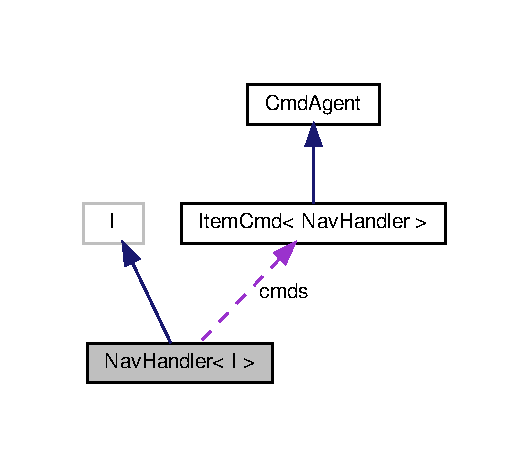
\includegraphics[width=254pt]{classNavHandler__coll__graph}
\end{center}
\end{figure}
\subsection*{Public Types}
\begin{DoxyCompactItemize}
\item 
\mbox{\Hypertarget{classNavHandler_a40be7497810e8f3660d19a4345bcdd80}\label{classNavHandler_a40be7497810e8f3660d19a4345bcdd80}} 
using {\bfseries This} = \hyperlink{classNavHandler}{Nav\+Handler}$<$ I $>$
\end{DoxyCompactItemize}
\subsection*{Public Member Functions}
\begin{DoxyCompactItemize}
\item 
\mbox{\Hypertarget{classNavHandler_aa3ca001d5ed2723e3b678388fc61ffe0}\label{classNavHandler_aa3ca001d5ed2723e3b678388fc61ffe0}} 
\hyperlink{structNavAgent}{Nav\+Agent} {\bfseries activate} ()
\end{DoxyCompactItemize}
\subsection*{Static Protected Attributes}
\begin{DoxyCompactItemize}
\item 
\mbox{\Hypertarget{classNavHandler_ab8a4970b41b11aae9d9d832063aff71f}\label{classNavHandler_ab8a4970b41b11aae9d9d832063aff71f}} 
static \hyperlink{structItemCmd}{Item\+Cmd}$<$ \hyperlink{classNavHandler}{This} $>$ {\bfseries cmds}
\end{DoxyCompactItemize}


\subsection{Detailed Description}
\subsubsection*{template$<$typename I$>$\newline
class Nav\+Handler$<$ I $>$}

The \hyperlink{classNavHandler}{Nav\+Handler} class allow menu item to receive navigation commands. Navigation functions are mapped automatically 

The documentation for this class was generated from the following files\+:\begin{DoxyCompactItemize}
\item 
src/menu/\hyperlink{item_8h}{item.\+h}\item 
src/menu/item.\+hpp\end{DoxyCompactItemize}

\hypertarget{structNavNode}{}\section{Nav\+Node Struct Reference}
\label{structNavNode}\index{Nav\+Node@{Nav\+Node}}


Inheritance diagram for Nav\+Node\+:\nopagebreak
\begin{figure}[H]
\begin{center}
\leavevmode
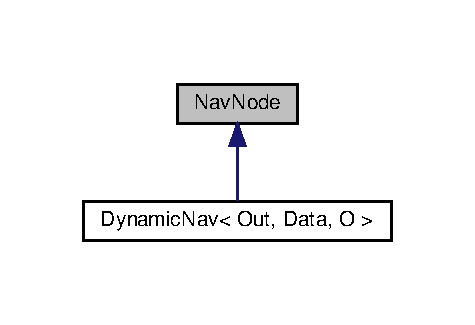
\includegraphics[width=228pt]{structNavNode__inherit__graph}
\end{center}
\end{figure}
\subsection*{Public Member Functions}
\begin{DoxyCompactItemize}
\item 
\mbox{\Hypertarget{structNavNode_acfd2cf12d4252148f39f2281923207fd}\label{structNavNode_acfd2cf12d4252148f39f2281923207fd}} 
virtual bool {\bfseries selected} (idx\+\_\+t) const
\item 
\mbox{\Hypertarget{structNavNode_a9865c81d79b6afb724bf2305745af4a8}\label{structNavNode_a9865c81d79b6afb724bf2305745af4a8}} 
virtual bool {\bfseries enabled} (idx\+\_\+t) const
\item 
\mbox{\Hypertarget{structNavNode_a5cd2a37ba693f1674f1be559832b81e7}\label{structNavNode_a5cd2a37ba693f1674f1be559832b81e7}} 
virtual Modes {\bfseries mode} () const
\item 
\mbox{\Hypertarget{structNavNode_a8ea0902eb8294a29b7128b7097ef5a6c}\label{structNavNode_a8ea0902eb8294a29b7128b7097ef5a6c}} 
virtual bool {\bfseries up} ()=0
\item 
\mbox{\Hypertarget{structNavNode_ab8aa8f5aea781ceb42fb107211c23eac}\label{structNavNode_ab8aa8f5aea781ceb42fb107211c23eac}} 
virtual bool {\bfseries down} ()=0
\item 
\mbox{\Hypertarget{structNavNode_a70c467220fab7c4648d6fd72213109c7}\label{structNavNode_a70c467220fab7c4648d6fd72213109c7}} 
virtual bool {\bfseries left} ()=0
\item 
\mbox{\Hypertarget{structNavNode_ad11086e7f82681cb6c47671021bfd5bc}\label{structNavNode_ad11086e7f82681cb6c47671021bfd5bc}} 
virtual bool {\bfseries right} ()=0
\item 
\mbox{\Hypertarget{structNavNode_ad76a28bf039c7ca36fc9343a9689cb0d}\label{structNavNode_ad76a28bf039c7ca36fc9343a9689cb0d}} 
virtual bool {\bfseries enter} ()=0
\item 
\mbox{\Hypertarget{structNavNode_a24fba244d14fde32cdaf81b277444ea7}\label{structNavNode_a24fba244d14fde32cdaf81b277444ea7}} 
virtual bool {\bfseries esc} ()=0
\end{DoxyCompactItemize}


The documentation for this struct was generated from the following file\+:\begin{DoxyCompactItemize}
\item 
src/menu/\hyperlink{base_8h}{base.\+h}\end{DoxyCompactItemize}

\hypertarget{classNavPos}{}\section{Nav\+Pos$<$ N $>$ Class Template Reference}
\label{classNavPos}\index{Nav\+Pos$<$ N $>$@{Nav\+Pos$<$ N $>$}}


{\ttfamily \#include $<$nav.\+h$>$}



Inheritance diagram for Nav\+Pos$<$ N $>$\+:\nopagebreak
\begin{figure}[H]
\begin{center}
\leavevmode
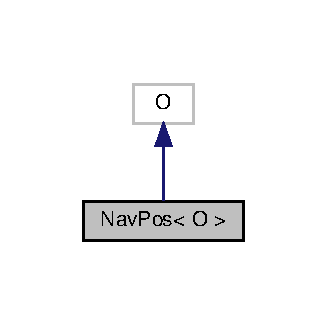
\includegraphics[width=157pt]{classNavPos__inherit__graph}
\end{center}
\end{figure}


Collaboration diagram for Nav\+Pos$<$ N $>$\+:\nopagebreak
\begin{figure}[H]
\begin{center}
\leavevmode
\includegraphics[width=157pt]{classNavPos__coll__graph}
\end{center}
\end{figure}
\subsection*{Public Types}
\begin{DoxyCompactItemize}
\item 
\mbox{\Hypertarget{classNavPos_aa32cd41af34948622157f83ab83d5c4a}\label{classNavPos_aa32cd41af34948622157f83ab83d5c4a}} 
using {\bfseries This} = \hyperlink{classNavPos}{Nav\+Pos}$<$ N $>$
\end{DoxyCompactItemize}
\subsection*{Public Member Functions}
\begin{DoxyCompactItemize}
\item 
\mbox{\Hypertarget{classNavPos_aebf5c7e017a6bccc4e8a1a87a790397e}\label{classNavPos_aebf5c7e017a6bccc4e8a1a87a790397e}} 
bool {\bfseries selected} (idx\+\_\+t idx) const
\item 
\mbox{\Hypertarget{classNavPos_ae26c7ff5d2fb3e0469daacccea51e49e}\label{classNavPos_ae26c7ff5d2fb3e0469daacccea51e49e}} 
{\footnotesize template$<$typename Nav $>$ }\\bool {\bfseries \+\_\+up} (Nav \&nav)
\item 
\mbox{\Hypertarget{classNavPos_a913487df01cc3893305d5ccd221d7c7a}\label{classNavPos_a913487df01cc3893305d5ccd221d7c7a}} 
{\footnotesize template$<$typename Nav $>$ }\\bool {\bfseries \+\_\+down} (Nav \&nav)
\item 
\mbox{\Hypertarget{classNavPos_a13da58ac811c5308ec0e6024774701b7}\label{classNavPos_a13da58ac811c5308ec0e6024774701b7}} 
idx\+\_\+t {\bfseries pos} ()
\item 
\mbox{\Hypertarget{classNavPos_aadbd4f1de82dbb156f90e90f8b196698}\label{classNavPos_aadbd4f1de82dbb156f90e90f8b196698}} 
{\footnotesize template$<$typename Nav $>$ }\\bool {\bfseries \+\_\+enter} (Nav \&nav)
\end{DoxyCompactItemize}
\subsection*{Protected Attributes}
\begin{DoxyCompactItemize}
\item 
\mbox{\Hypertarget{classNavPos_a99798e57e3b5333836e570d125a6ebed}\label{classNavPos_a99798e57e3b5333836e570d125a6ebed}} 
idx\+\_\+t {\bfseries at}
\end{DoxyCompactItemize}


\subsection{Detailed Description}
\subsubsection*{template$<$typename N = Drift$<$$>$$>$\newline
class Nav\+Pos$<$ N $>$}

The \hyperlink{classNavPos}{Nav\+Pos} class holds selected item index, is a primitive navigation functionality 

The documentation for this class was generated from the following file\+:\begin{DoxyCompactItemize}
\item 
src/menu/\hyperlink{nav_8h}{nav.\+h}\end{DoxyCompactItemize}

\hypertarget{structNil}{}\section{Nil Struct Reference}
\label{structNil}\index{Nil@{Nil}}


Inheritance diagram for Nil\+:\nopagebreak
\begin{figure}[H]
\begin{center}
\leavevmode
\includegraphics[width=154pt]{structNil__inherit__graph}
\end{center}
\end{figure}


The documentation for this struct was generated from the following file\+:\begin{DoxyCompactItemize}
\item 
src/menu/\hyperlink{base_8h}{base.\+h}\end{DoxyCompactItemize}

\hypertarget{classNumField}{}\section{Num\+Field$<$ T, I $>$ Class Template Reference}
\label{classNumField}\index{Num\+Field$<$ T, I $>$@{Num\+Field$<$ T, I $>$}}


{\ttfamily \#include $<$num\+Field.\+h$>$}



Inheritance diagram for Num\+Field$<$ T, I $>$\+:\nopagebreak
\begin{figure}[H]
\begin{center}
\leavevmode
\includegraphics[width=172pt]{classNumField__inherit__graph}
\end{center}
\end{figure}


Collaboration diagram for Num\+Field$<$ T, I $>$\+:\nopagebreak
\begin{figure}[H]
\begin{center}
\leavevmode
\includegraphics[width=172pt]{classNumField__coll__graph}
\end{center}
\end{figure}
\subsection*{Public Member Functions}
\begin{DoxyCompactItemize}
\item 
\mbox{\Hypertarget{classNumField_ac31c0e5c4a8dfc82780e643140c608f8}\label{classNumField_ac31c0e5c4a8dfc82780e643140c608f8}} 
{\bfseries Num\+Field} (T \&var, T l, T h, T s, T t=0)
\item 
\mbox{\Hypertarget{classNumField_a0f94b131552e24e24516ed07c3345564}\label{classNumField_a0f94b131552e24e24516ed07c3345564}} 
void {\bfseries out} (\hyperlink{structMenuOut}{Menu\+Out} \&o) const
\item 
\mbox{\Hypertarget{classNumField_a1fc5409fdd22fbca9ffcfdbe90cf9929}\label{classNumField_a1fc5409fdd22fbca9ffcfdbe90cf9929}} 
bool {\bfseries up} ()
\item 
\mbox{\Hypertarget{classNumField_ae0bd47d4969d695fa7cff81e44d4dff9}\label{classNumField_ae0bd47d4969d695fa7cff81e44d4dff9}} 
bool {\bfseries down} ()
\item 
\mbox{\Hypertarget{classNumField_abe795198b4e2b95502933164d3cd64ec}\label{classNumField_abe795198b4e2b95502933164d3cd64ec}} 
bool {\bfseries enter} ()
\item 
\mbox{\Hypertarget{classNumField_ae7697ba53072d3eacf0a041c93140f4e}\label{classNumField_ae7697ba53072d3eacf0a041c93140f4e}} 
bool {\bfseries esc} ()
\end{DoxyCompactItemize}
\subsection*{Protected Attributes}
\begin{DoxyCompactItemize}
\item 
\mbox{\Hypertarget{classNumField_a1c72fd5bc1775e6cfaed2b4594ac0700}\label{classNumField_a1c72fd5bc1775e6cfaed2b4594ac0700}} 
bool {\bfseries tunning} =false
\item 
\mbox{\Hypertarget{classNumField_a548ac7ac150b3b12811bfef53d9636a5}\label{classNumField_a548ac7ac150b3b12811bfef53d9636a5}} 
T $\ast$ {\bfseries value}
\item 
\mbox{\Hypertarget{classNumField_ad17a73e2250ebbd5dda7ee3a79dfb522}\label{classNumField_ad17a73e2250ebbd5dda7ee3a79dfb522}} 
T {\bfseries reflex}
\item 
\mbox{\Hypertarget{classNumField_a9e04257f27cf53402e8d787b6a1d561e}\label{classNumField_a9e04257f27cf53402e8d787b6a1d561e}} 
T {\bfseries low}
\item 
\mbox{\Hypertarget{classNumField_ab40ba1ee654bc48e827b78297b384714}\label{classNumField_ab40ba1ee654bc48e827b78297b384714}} 
T {\bfseries high}
\item 
\mbox{\Hypertarget{classNumField_acd99c4f2a3c0b3477535399485782827}\label{classNumField_acd99c4f2a3c0b3477535399485782827}} 
T {\bfseries step}
\item 
\mbox{\Hypertarget{classNumField_af28a046a1c71b17e8ac7ed17abba03ff}\label{classNumField_af28a046a1c71b17e8ac7ed17abba03ff}} 
T {\bfseries tune}
\end{DoxyCompactItemize}


\subsection{Detailed Description}
\subsubsection*{template$<$typename T, typename I = Empty$<$$>$$>$\newline
class Num\+Field$<$ T, I $>$}

The \hyperlink{classNumField}{Num\+Field} class links to any numeric type variable and allows changing it between the validation range 

The documentation for this class was generated from the following file\+:\begin{DoxyCompactItemize}
\item 
src/menu/comp/\hyperlink{numField_8h}{num\+Field.\+h}\end{DoxyCompactItemize}

\hypertarget{classOutList}{}\section{Out\+List$<$ O, OO $>$ Class Template Reference}
\label{classOutList}\index{Out\+List$<$ O, O\+O $>$@{Out\+List$<$ O, O\+O $>$}}
\subsection*{Public Types}
\begin{DoxyCompactItemize}
\item 
\mbox{\Hypertarget{classOutList_a2d2673aa6b42f90c3d9c355b169c3d07}\label{classOutList_a2d2673aa6b42f90c3d9c355b169c3d07}} 
using {\bfseries This} = \hyperlink{classOutList}{Out\+List}$<$ O, O\+O... $>$
\item 
\mbox{\Hypertarget{classOutList_a43d76f077a12b8b4375b2044cde570c9}\label{classOutList_a43d76f077a12b8b4375b2044cde570c9}} 
using {\bfseries Next} = \hyperlink{classOutList}{Out\+List}$<$ O\+O... $>$
\end{DoxyCompactItemize}
\subsection*{Public Member Functions}
\begin{DoxyCompactItemize}
\item 
\mbox{\Hypertarget{classOutList_a545b6a67dfda40046004d50096215c2d}\label{classOutList_a545b6a67dfda40046004d50096215c2d}} 
{\footnotesize template$<$typename Nav , typename Out , typename I $>$ }\\void {\bfseries print\+Menu} (Nav \&nav, Out \&out, I \&i)
\end{DoxyCompactItemize}
\subsection*{Protected Attributes}
\begin{DoxyCompactItemize}
\item 
\mbox{\Hypertarget{classOutList_ac43c0f0f67e2bf8549bfbea48bcfb3c7}\label{classOutList_ac43c0f0f67e2bf8549bfbea48bcfb3c7}} 
\hyperlink{classOutList}{Next} {\bfseries next}
\end{DoxyCompactItemize}


The documentation for this class was generated from the following file\+:\begin{DoxyCompactItemize}
\item 
src/menu/\+I\+O/\hyperlink{outList_8h}{out\+List.\+h}\end{DoxyCompactItemize}

\hypertarget{classOutList_3_01O_01_4}{}\section{Out\+List$<$ O $>$ Class Template Reference}
\label{classOutList_3_01O_01_4}\index{Out\+List$<$ O $>$@{Out\+List$<$ O $>$}}


Inheritance diagram for Out\+List$<$ O $>$\+:\nopagebreak
\begin{figure}[H]
\begin{center}
\leavevmode
\includegraphics[width=154pt]{classOutList_3_01O_01_4__inherit__graph}
\end{center}
\end{figure}


Collaboration diagram for Out\+List$<$ O $>$\+:\nopagebreak
\begin{figure}[H]
\begin{center}
\leavevmode
\includegraphics[width=154pt]{classOutList_3_01O_01_4__coll__graph}
\end{center}
\end{figure}
\subsection*{Public Member Functions}
\begin{DoxyCompactItemize}
\item 
\mbox{\Hypertarget{classOutList_3_01O_01_4_a1807db22ab1b84545af1196b1713204f}\label{classOutList_3_01O_01_4_a1807db22ab1b84545af1196b1713204f}} 
{\footnotesize template$<$typename Nav , typename Out , typename I $>$ }\\void {\bfseries print\+Menu} (Nav \&nav, Out \&out, I \&i)
\end{DoxyCompactItemize}


The documentation for this class was generated from the following file\+:\begin{DoxyCompactItemize}
\item 
src/menu/\+I\+O/\hyperlink{outList_8h}{out\+List.\+h}\end{DoxyCompactItemize}

\hypertarget{structOutOp}{}\section{Out\+Op$<$ Out\+Ops $>$ Struct Template Reference}
\label{structOutOp}\index{Out\+Op$<$ Out\+Ops $>$@{Out\+Op$<$ Out\+Ops $>$}}


The documentation for this struct was generated from the following file\+:\begin{DoxyCompactItemize}
\item 
src/menu/\hyperlink{base_8h}{base.\+h}\end{DoxyCompactItemize}

\hypertarget{structPrompt}{}\section{Prompt$<$ O $>$ Struct Template Reference}
\label{structPrompt}\index{Prompt$<$ O $>$@{Prompt$<$ O $>$}}


{\ttfamily \#include $<$item.\+h$>$}



Inheritance diagram for Prompt$<$ O $>$\+:\nopagebreak
\begin{figure}[H]
\begin{center}
\leavevmode
\includegraphics[width=164pt]{structPrompt__inherit__graph}
\end{center}
\end{figure}


Collaboration diagram for Prompt$<$ O $>$\+:\nopagebreak
\begin{figure}[H]
\begin{center}
\leavevmode
\includegraphics[width=164pt]{structPrompt__coll__graph}
\end{center}
\end{figure}
\subsection*{Public Member Functions}
\begin{DoxyCompactItemize}
\item 
\mbox{\Hypertarget{structPrompt_a00ec62ca84f509b26898137e2df772f9}\label{structPrompt_a00ec62ca84f509b26898137e2df772f9}} 
void {\bfseries print\+Item} (\hyperlink{structNavNode}{Nav\+Node} \&nav, \hyperlink{structMenuOut}{Menu\+Out} \&out, idx\+\_\+t n) override
\item 
\mbox{\Hypertarget{structPrompt_a2ce155e8c7582809fc15802e06954fab}\label{structPrompt_a2ce155e8c7582809fc15802e06954fab}} 
void {\bfseries print} (\hyperlink{structNavNode}{Nav\+Node} \&nav, \hyperlink{structMenuOut}{Menu\+Out} \&out) override
\item 
\mbox{\Hypertarget{structPrompt_a40a2fe7ed21396bedd6b65b2db5400a6}\label{structPrompt_a40a2fe7ed21396bedd6b65b2db5400a6}} 
void {\bfseries enable} (idx\+\_\+t n, bool b) override
\item 
\mbox{\Hypertarget{structPrompt_a4f769df1e55e65f6a07d297efb15cf44}\label{structPrompt_a4f769df1e55e65f6a07d297efb15cf44}} 
virtual bool {\bfseries enabled} (idx\+\_\+t n) const override
\item 
\mbox{\Hypertarget{structPrompt_aa5befa00eeae10f725e06c2c087d177d}\label{structPrompt_aa5befa00eeae10f725e06c2c087d177d}} 
bool {\bfseries activate} () override
\item 
\mbox{\Hypertarget{structPrompt_a6245d593b4c924276faeb8b5b4424e53}\label{structPrompt_a6245d593b4c924276faeb8b5b4424e53}} 
bool {\bfseries activate} (idx\+\_\+t n) override
\end{DoxyCompactItemize}


\subsection{Detailed Description}
\subsubsection*{template$<$typename O$>$\newline
struct Prompt$<$ O $>$}

The \hyperlink{structPrompt}{Prompt} class represents a generic virtual menu item. This class allows \hyperlink{structPrompt}{Prompt} pointers to be stored on a list as they all implement the same interface. This will adapts a composition to the virtual interface. 

The documentation for this struct was generated from the following file\+:\begin{DoxyCompactItemize}
\item 
src/menu/\hyperlink{item_8h}{item.\+h}\end{DoxyCompactItemize}

\hypertarget{classRangePanel}{}\section{Range\+Panel$<$ O $>$ Class Template Reference}
\label{classRangePanel}\index{Range\+Panel$<$ O $>$@{Range\+Panel$<$ O $>$}}


{\ttfamily \#include $<$panels.\+h$>$}



Inheritance diagram for Range\+Panel$<$ O $>$\+:\nopagebreak
\begin{figure}[H]
\begin{center}
\leavevmode
\includegraphics[width=175pt]{classRangePanel__inherit__graph}
\end{center}
\end{figure}


Collaboration diagram for Range\+Panel$<$ O $>$\+:\nopagebreak
\begin{figure}[H]
\begin{center}
\leavevmode
\includegraphics[width=175pt]{classRangePanel__coll__graph}
\end{center}
\end{figure}
\subsection*{Public Member Functions}
\begin{DoxyCompactItemize}
\item 
\mbox{\Hypertarget{classRangePanel_a6e9afb303bbe3f59bbc82363aa9642f9}\label{classRangePanel_a6e9afb303bbe3f59bbc82363aa9642f9}} 
idx\+\_\+t {\bfseries top} () const
\item 
\mbox{\Hypertarget{classRangePanel_aecc0841ba198f660e898f7c6e03f1aca}\label{classRangePanel_aecc0841ba198f660e898f7c6e03f1aca}} 
void {\bfseries set\+Top} (idx\+\_\+t n)
\end{DoxyCompactItemize}
\subsection*{Static Public Member Functions}
\begin{DoxyCompactItemize}
\item 
\mbox{\Hypertarget{classRangePanel_ab5afc2b81ec2f1d43e4c13d103168e7c}\label{classRangePanel_ab5afc2b81ec2f1d43e4c13d103168e7c}} 
static constexpr bool {\bfseries is\+Range} ()
\end{DoxyCompactItemize}
\subsection*{Protected Attributes}
\begin{DoxyCompactItemize}
\item 
\mbox{\Hypertarget{classRangePanel_ae51c75c38328641275d6af9c61bd838f}\label{classRangePanel_ae51c75c38328641275d6af9c61bd838f}} 
idx\+\_\+t {\bfseries top\+Line} =0
\end{DoxyCompactItemize}


\subsection{Detailed Description}
\subsubsection*{template$<$typename O$>$\newline
class Range\+Panel$<$ O $>$}

The \hyperlink{classRangePanel}{Range\+Panel} class is different than a scroll viewport as it refers to the top line of the menu structure. Minimize printing code on line menus. 

The documentation for this class was generated from the following file\+:\begin{DoxyCompactItemize}
\item 
src/menu/\hyperlink{panels_8h}{panels.\+h}\end{DoxyCompactItemize}

\hypertarget{structRawOut}{}\section{Raw\+Out$<$ Dev, dev, O $>$ Struct Template Reference}
\label{structRawOut}\index{Raw\+Out$<$ Dev, dev, O $>$@{Raw\+Out$<$ Dev, dev, O $>$}}


Inheritance diagram for Raw\+Out$<$ Dev, dev, O $>$\+:\nopagebreak
\begin{figure}[H]
\begin{center}
\leavevmode
\includegraphics[width=204pt]{structRawOut__inherit__graph}
\end{center}
\end{figure}


Collaboration diagram for Raw\+Out$<$ Dev, dev, O $>$\+:\nopagebreak
\begin{figure}[H]
\begin{center}
\leavevmode
\includegraphics[width=204pt]{structRawOut__coll__graph}
\end{center}
\end{figure}
\subsection*{Static Public Member Functions}
\begin{DoxyCompactItemize}
\item 
\mbox{\Hypertarget{structRawOut_ad4171805d902b301ea83e7bd62787f06}\label{structRawOut_ad4171805d902b301ea83e7bd62787f06}} 
{\footnotesize template$<$typename T $>$ }\\static void {\bfseries raw} (T o)
\end{DoxyCompactItemize}


The documentation for this struct was generated from the following file\+:\begin{DoxyCompactItemize}
\item 
src/menu/\hyperlink{out_8h}{out.\+h}\end{DoxyCompactItemize}

\hypertarget{structSerialOut}{}\section{Serial\+Out$<$ Dev, dev, O $>$ Struct Template Reference}
\label{structSerialOut}\index{Serial\+Out$<$ Dev, dev, O $>$@{Serial\+Out$<$ Dev, dev, O $>$}}


Inheritance diagram for Serial\+Out$<$ Dev, dev, O $>$\+:\nopagebreak
\begin{figure}[H]
\begin{center}
\leavevmode
\includegraphics[width=214pt]{structSerialOut__inherit__graph}
\end{center}
\end{figure}


Collaboration diagram for Serial\+Out$<$ Dev, dev, O $>$\+:\nopagebreak
\begin{figure}[H]
\begin{center}
\leavevmode
\includegraphics[width=214pt]{structSerialOut__coll__graph}
\end{center}
\end{figure}
\subsection*{Static Public Member Functions}
\begin{DoxyCompactItemize}
\item 
\mbox{\Hypertarget{structSerialOut_a983a053fdb8a39e70fa4dae9b2001dfd}\label{structSerialOut_a983a053fdb8a39e70fa4dae9b2001dfd}} 
static void {\bfseries nl} ()
\item 
\mbox{\Hypertarget{structSerialOut_a13b599107c4c409f915a2eacf22f67d6}\label{structSerialOut_a13b599107c4c409f915a2eacf22f67d6}} 
{\footnotesize template$<$typename T $>$ }\\static void {\bfseries raw} (T o)
\end{DoxyCompactItemize}


The documentation for this struct was generated from the following file\+:\begin{DoxyCompactItemize}
\item 
src/menu/\+I\+O/\hyperlink{serialOut_8h}{serial\+Out.\+h}\end{DoxyCompactItemize}

\hypertarget{classStaticMenu}{}\section{Static\+Menu$<$ I, II $>$ Class Template Reference}
\label{classStaticMenu}\index{Static\+Menu$<$ I, I\+I $>$@{Static\+Menu$<$ I, I\+I $>$}}


{\ttfamily \#include $<$item.\+h$>$}

\subsection*{Public Types}
\begin{DoxyCompactItemize}
\item 
\mbox{\Hypertarget{classStaticMenu_af5a92e27a1dc146ef1a6facfb870b245}\label{classStaticMenu_af5a92e27a1dc146ef1a6facfb870b245}} 
using {\bfseries This} = \hyperlink{classStaticMenu}{Static\+Menu}$<$ I $>$
\item 
\mbox{\Hypertarget{classStaticMenu_a85c856832cde6a24cdfff1fa28891017}\label{classStaticMenu_a85c856832cde6a24cdfff1fa28891017}} 
using {\bfseries Next} = \hyperlink{classStaticMenu}{Static\+Menu}$<$ I\+I... $>$
\end{DoxyCompactItemize}
\subsection*{Public Member Functions}
\begin{DoxyCompactItemize}
\item 
\mbox{\Hypertarget{classStaticMenu_a7b958c98761a7974d927041f9c659779}\label{classStaticMenu_a7b958c98761a7974d927041f9c659779}} 
constexpr idx\+\_\+t {\bfseries size} ()
\item 
\mbox{\Hypertarget{classStaticMenu_a0cb879980a1886111d9d6307510ca7c9}\label{classStaticMenu_a0cb879980a1886111d9d6307510ca7c9}} 
{\footnotesize template$<$typename Nav , typename Out $>$ }\\void {\bfseries print\+Item} (Nav \&nav, Out \&out, idx\+\_\+t n)
\item 
\mbox{\Hypertarget{classStaticMenu_ad92d5faa9b949038b1fbfe77e20a6674}\label{classStaticMenu_ad92d5faa9b949038b1fbfe77e20a6674}} 
void {\bfseries enable} (idx\+\_\+t n, bool o)
\item 
\mbox{\Hypertarget{classStaticMenu_ab7a3a6c422252f5d2cc467bed2d36e2c}\label{classStaticMenu_ab7a3a6c422252f5d2cc467bed2d36e2c}} 
bool {\bfseries enabled} (idx\+\_\+t n) const
\item 
\mbox{\Hypertarget{classStaticMenu_a6f5156578dd2e98db3c40c89ed39d95c}\label{classStaticMenu_a6f5156578dd2e98db3c40c89ed39d95c}} 
\hyperlink{structNavAgent}{Nav\+Agent} {\bfseries activate\+Item} (idx\+\_\+t n)
\end{DoxyCompactItemize}
\subsection*{Protected Attributes}
\begin{DoxyCompactItemize}
\item 
\mbox{\Hypertarget{classStaticMenu_aee7481e4086bdd909f05eb80177ade99}\label{classStaticMenu_aee7481e4086bdd909f05eb80177ade99}} 
\hyperlink{classStaticMenu}{Next} {\bfseries next}
\end{DoxyCompactItemize}


\subsection{Detailed Description}
\subsubsection*{template$<$typename I, typename... II$>$\newline
class Static\+Menu$<$ I, I\+I $>$}

The \hyperlink{classStaticMenu}{Static\+Menu} class represents a compile time menu structure. 

The documentation for this class was generated from the following file\+:\begin{DoxyCompactItemize}
\item 
src/menu/\hyperlink{item_8h}{item.\+h}\end{DoxyCompactItemize}

\hypertarget{structStaticMenu_3_01I_01_4}{}\section{Static\+Menu$<$ I $>$ Struct Template Reference}
\label{structStaticMenu_3_01I_01_4}\index{Static\+Menu$<$ I $>$@{Static\+Menu$<$ I $>$}}


{\ttfamily \#include $<$item.\+h$>$}



Inheritance diagram for Static\+Menu$<$ I $>$\+:\nopagebreak
\begin{figure}[H]
\begin{center}
\leavevmode
\includegraphics[width=167pt]{structStaticMenu_3_01I_01_4__inherit__graph}
\end{center}
\end{figure}


Collaboration diagram for Static\+Menu$<$ I $>$\+:\nopagebreak
\begin{figure}[H]
\begin{center}
\leavevmode
\includegraphics[width=167pt]{structStaticMenu_3_01I_01_4__coll__graph}
\end{center}
\end{figure}
\subsection*{Public Types}
\begin{DoxyCompactItemize}
\item 
\mbox{\Hypertarget{structStaticMenu_3_01I_01_4_add0be905f5b426cf7b9cdec9c21683d3}\label{structStaticMenu_3_01I_01_4_add0be905f5b426cf7b9cdec9c21683d3}} 
using {\bfseries This} = \hyperlink{classStaticMenu}{Static\+Menu}$<$ I $>$
\end{DoxyCompactItemize}
\subsection*{Public Member Functions}
\begin{DoxyCompactItemize}
\item 
\mbox{\Hypertarget{structStaticMenu_3_01I_01_4_a4449b1842a30593dc7236d44be58651b}\label{structStaticMenu_3_01I_01_4_a4449b1842a30593dc7236d44be58651b}} 
{\footnotesize template$<$typename Nav , typename Out $>$ }\\void {\bfseries print} (Nav \&nav, Out \&out)
\item 
\mbox{\Hypertarget{structStaticMenu_3_01I_01_4_a67a791084edf441d625a12fe7d649392}\label{structStaticMenu_3_01I_01_4_a67a791084edf441d625a12fe7d649392}} 
{\footnotesize template$<$typename Nav , typename Out $>$ }\\void {\bfseries print\+Item} (Nav \&nav, Out \&out, idx\+\_\+t)
\item 
\mbox{\Hypertarget{structStaticMenu_3_01I_01_4_ae67af5d6b2cc7630b7ab12e2e1bc4dd1}\label{structStaticMenu_3_01I_01_4_ae67af5d6b2cc7630b7ab12e2e1bc4dd1}} 
bool {\bfseries enabled} (idx\+\_\+t n) const
\item 
\mbox{\Hypertarget{structStaticMenu_3_01I_01_4_afa003d349bc90ab91e5f94d44593879c}\label{structStaticMenu_3_01I_01_4_afa003d349bc90ab91e5f94d44593879c}} 
void {\bfseries enable} (idx\+\_\+t n, bool o)
\end{DoxyCompactItemize}
\subsection*{Static Public Member Functions}
\begin{DoxyCompactItemize}
\item 
\mbox{\Hypertarget{structStaticMenu_3_01I_01_4_a070f528540a846fa3280e7827b9de47a}\label{structStaticMenu_3_01I_01_4_a070f528540a846fa3280e7827b9de47a}} 
static constexpr idx\+\_\+t {\bfseries size} ()
\end{DoxyCompactItemize}


\subsection{Detailed Description}
\subsubsection*{template$<$typename I$>$\newline
struct Static\+Menu$<$ I $>$}

The \hyperlink{classStaticMenu}{Static\+Menu} specialization class represents the last element of a compile-\/time menu content chain. 

The documentation for this struct was generated from the following file\+:\begin{DoxyCompactItemize}
\item 
src/menu/\hyperlink{item_8h}{item.\+h}\end{DoxyCompactItemize}

\hypertarget{classStaticNav}{}\section{Static\+Nav$<$ Out, Data, O $>$ Class Template Reference}
\label{classStaticNav}\index{Static\+Nav$<$ Out, Data, O $>$@{Static\+Nav$<$ Out, Data, O $>$}}


Inheritance diagram for Static\+Nav$<$ Out, Data, O $>$\+:\nopagebreak
\begin{figure}[H]
\begin{center}
\leavevmode
\includegraphics[width=214pt]{classStaticNav__inherit__graph}
\end{center}
\end{figure}


Collaboration diagram for Static\+Nav$<$ Out, Data, O $>$\+:\nopagebreak
\begin{figure}[H]
\begin{center}
\leavevmode
\includegraphics[width=323pt]{classStaticNav__coll__graph}
\end{center}
\end{figure}
\subsection*{Public Types}
\begin{DoxyCompactItemize}
\item 
\mbox{\Hypertarget{classStaticNav_a2f3bcbf88851bf7f3a996f601a4e7b2a}\label{classStaticNav_a2f3bcbf88851bf7f3a996f601a4e7b2a}} 
using {\bfseries Base} = \hyperlink{classNavBase}{Nav\+Base}$<$ Out, O $>$
\item 
\mbox{\Hypertarget{classStaticNav_a0cd2b778a1ae3fdb1ce623cdcc0ff648}\label{classStaticNav_a0cd2b778a1ae3fdb1ce623cdcc0ff648}} 
using {\bfseries This} = \hyperlink{classStaticNav}{Static\+Nav}$<$ Out, Data, O $>$
\end{DoxyCompactItemize}
\subsection*{Public Member Functions}
\begin{DoxyCompactItemize}
\item 
\mbox{\Hypertarget{classStaticNav_a03fef842273f435c094e09d9f11870f1}\label{classStaticNav_a03fef842273f435c094e09d9f11870f1}} 
void {\bfseries set\+Target} (Data d)
\item 
\mbox{\Hypertarget{classStaticNav_adf54cd9e3451116ed8c0c38a964e23ae}\label{classStaticNav_adf54cd9e3451116ed8c0c38a964e23ae}} 
void {\bfseries print\+Menu} ()
\item 
\mbox{\Hypertarget{classStaticNav_a53b3197546f76215945321ee88a60fa9}\label{classStaticNav_a53b3197546f76215945321ee88a60fa9}} 
idx\+\_\+t {\bfseries size} ()
\item 
\mbox{\Hypertarget{classStaticNav_a7ba688dae4101e447866d1fa046d3764}\label{classStaticNav_a7ba688dae4101e447866d1fa046d3764}} 
void {\bfseries enable} (idx\+\_\+t n, bool o)
\item 
\mbox{\Hypertarget{classStaticNav_a98ccf85a6268a4c6cab16f80589511c9}\label{classStaticNav_a98ccf85a6268a4c6cab16f80589511c9}} 
bool {\bfseries enabled} (idx\+\_\+t n)
\item 
\mbox{\Hypertarget{classStaticNav_acdf792e96538be6b67f9e6c78fd8117f}\label{classStaticNav_acdf792e96538be6b67f9e6c78fd8117f}} 
bool {\bfseries activate} ()
\item 
\mbox{\Hypertarget{classStaticNav_a9b0a9573993822097b3370a528ab8828}\label{classStaticNav_a9b0a9573993822097b3370a528ab8828}} 
bool {\bfseries activate} (idx\+\_\+t n)
\end{DoxyCompactItemize}
\subsection*{Protected Attributes}
\begin{DoxyCompactItemize}
\item 
\mbox{\Hypertarget{classStaticNav_a6870b765b0896ec89064d74e816f32a3}\label{classStaticNav_a6870b765b0896ec89064d74e816f32a3}} 
Data {\bfseries data}
\end{DoxyCompactItemize}


The documentation for this class was generated from the following file\+:\begin{DoxyCompactItemize}
\item 
src/menu/\hyperlink{nav_8h}{nav.\+h}\end{DoxyCompactItemize}

\hypertarget{structStaticPanel}{}\section{Static\+Panel$<$ x, y, w, h, O $>$ Struct Template Reference}
\label{structStaticPanel}\index{Static\+Panel$<$ x, y, w, h, O $>$@{Static\+Panel$<$ x, y, w, h, O $>$}}


{\ttfamily \#include $<$panels.\+h$>$}



Inheritance diagram for Static\+Panel$<$ x, y, w, h, O $>$\+:\nopagebreak
\begin{figure}[H]
\begin{center}
\leavevmode
\includegraphics[width=175pt]{structStaticPanel__inherit__graph}
\end{center}
\end{figure}


Collaboration diagram for Static\+Panel$<$ x, y, w, h, O $>$\+:\nopagebreak
\begin{figure}[H]
\begin{center}
\leavevmode
\includegraphics[width=175pt]{structStaticPanel__coll__graph}
\end{center}
\end{figure}
\subsection*{Static Public Member Functions}
\begin{DoxyCompactItemize}
\item 
\mbox{\Hypertarget{structStaticPanel_a212fd5e5bcdcd315954c142444fe58cd}\label{structStaticPanel_a212fd5e5bcdcd315954c142444fe58cd}} 
static constexpr idx\+\_\+t {\bfseries orgX} ()
\item 
\mbox{\Hypertarget{structStaticPanel_af02d741f125c68e62f4136d113d1d509}\label{structStaticPanel_af02d741f125c68e62f4136d113d1d509}} 
static constexpr idx\+\_\+t {\bfseries orgY} ()
\item 
\mbox{\Hypertarget{structStaticPanel_a282e4e37cb469aa22c941ae601814dfc}\label{structStaticPanel_a282e4e37cb469aa22c941ae601814dfc}} 
static constexpr idx\+\_\+t {\bfseries width} ()
\item 
\mbox{\Hypertarget{structStaticPanel_a25776cf952e42e10edb36235744d1326}\label{structStaticPanel_a25776cf952e42e10edb36235744d1326}} 
static constexpr idx\+\_\+t {\bfseries height} ()
\item 
\mbox{\Hypertarget{structStaticPanel_a5f81c3d0f56d0cd0c898cccd7df0af5d}\label{structStaticPanel_a5f81c3d0f56d0cd0c898cccd7df0af5d}} 
static constexpr idx\+\_\+t {\bfseries posX} ()
\item 
\mbox{\Hypertarget{structStaticPanel_a9ab23a0b5f4350ca53442bfe18abb83a}\label{structStaticPanel_a9ab23a0b5f4350ca53442bfe18abb83a}} 
static constexpr idx\+\_\+t {\bfseries posY} ()
\item 
\mbox{\Hypertarget{structStaticPanel_a5f061e3f28cf7ef9b243d010d61f64fe}\label{structStaticPanel_a5f061e3f28cf7ef9b243d010d61f64fe}} 
static constexpr idx\+\_\+t {\bfseries freeX} ()
\item 
\mbox{\Hypertarget{structStaticPanel_a3c80c3856c529db7e75985a0dc256aba}\label{structStaticPanel_a3c80c3856c529db7e75985a0dc256aba}} 
static constexpr idx\+\_\+t {\bfseries freeY} ()
\item 
\mbox{\Hypertarget{structStaticPanel_ab079b6885119d57fa9b19fde200f6d08}\label{structStaticPanel_ab079b6885119d57fa9b19fde200f6d08}} 
static constexpr idx\+\_\+t {\bfseries free} ()
\item 
\mbox{\Hypertarget{structStaticPanel_a543575d0480cce8c0e3e34fbdff5c6b8}\label{structStaticPanel_a543575d0480cce8c0e3e34fbdff5c6b8}} 
static void {\bfseries useX} (idx\+\_\+t ux=1)
\item 
\mbox{\Hypertarget{structStaticPanel_aa74dc84981d0ae6f1e5c6a8892b5eea0}\label{structStaticPanel_aa74dc84981d0ae6f1e5c6a8892b5eea0}} 
static void {\bfseries useY} (idx\+\_\+t uy=1)
\end{DoxyCompactItemize}


\subsection{Detailed Description}
\subsubsection*{template$<$idx\+\_\+t x, idx\+\_\+t y, idx\+\_\+t w, idx\+\_\+t h, typename O$>$\newline
struct Static\+Panel$<$ x, y, w, h, O $>$}

The \hyperlink{structStaticPanel}{Static\+Panel} class describes output geometry, may be whole device, but must not exceed. It has origin coordinates to be displaced around 

The documentation for this struct was generated from the following file\+:\begin{DoxyCompactItemize}
\item 
src/menu/\hyperlink{panels_8h}{panels.\+h}\end{DoxyCompactItemize}

\hypertarget{structStaticText}{}\section{Static\+Text$<$ text, I $>$ Struct Template Reference}
\label{structStaticText}\index{Static\+Text$<$ text, I $>$@{Static\+Text$<$ text, I $>$}}


{\ttfamily \#include $<$item.\+h$>$}



Inheritance diagram for Static\+Text$<$ text, I $>$\+:\nopagebreak
\begin{figure}[H]
\begin{center}
\leavevmode
\includegraphics[width=185pt]{structStaticText__inherit__graph}
\end{center}
\end{figure}


Collaboration diagram for Static\+Text$<$ text, I $>$\+:\nopagebreak
\begin{figure}[H]
\begin{center}
\leavevmode
\includegraphics[width=185pt]{structStaticText__coll__graph}
\end{center}
\end{figure}
\subsection*{Public Member Functions}
\begin{DoxyCompactItemize}
\item 
\mbox{\Hypertarget{structStaticText_a4a8e1297ef0651fdeb03b6b78fd65ae8}\label{structStaticText_a4a8e1297ef0651fdeb03b6b78fd65ae8}} 
{\footnotesize template$<$typename Nav , typename Out $>$ }\\void {\bfseries print} (Nav \&nav, Out \&out)
\end{DoxyCompactItemize}


\subsection{Detailed Description}
\subsubsection*{template$<$const char $\ast$$\ast$ text, typename I = Empty$<$$>$$>$\newline
struct Static\+Text$<$ text, I $>$}

The \hyperlink{structStaticText}{Static\+Text} class provides code stored constant strings. 

The documentation for this struct was generated from the following file\+:\begin{DoxyCompactItemize}
\item 
src/menu/\hyperlink{item_8h}{item.\+h}\end{DoxyCompactItemize}

\hypertarget{structTextFmt}{}\section{Text\+Fmt$<$ O $>$ Struct Template Reference}
\label{structTextFmt}\index{Text\+Fmt$<$ O $>$@{Text\+Fmt$<$ O $>$}}


Inheritance diagram for Text\+Fmt$<$ O $>$\+:\nopagebreak
\begin{figure}[H]
\begin{center}
\leavevmode
\includegraphics[width=159pt]{structTextFmt__inherit__graph}
\end{center}
\end{figure}


Collaboration diagram for Text\+Fmt$<$ O $>$\+:\nopagebreak
\begin{figure}[H]
\begin{center}
\leavevmode
\includegraphics[width=159pt]{structTextFmt__coll__graph}
\end{center}
\end{figure}
\subsection*{Public Member Functions}
\begin{DoxyCompactItemize}
\item 
\mbox{\Hypertarget{structTextFmt_a5a449272db2ae1fce810e0068b4c03c5}\label{structTextFmt_a5a449272db2ae1fce810e0068b4c03c5}} 
{\footnotesize template$<$bool io, typename Nav , typename Out , typename I $>$ }\\void {\bfseries fmt\+Cursor} (Nav \&nav, Out \&out, I \&i, idx\+\_\+t n)
\end{DoxyCompactItemize}
\subsection*{Static Public Member Functions}
\begin{DoxyCompactItemize}
\item 
\mbox{\Hypertarget{structTextFmt_a5f1cbec0608bca7db5f489239c041f9e}\label{structTextFmt_a5f1cbec0608bca7db5f489239c041f9e}} 
{\footnotesize template$<$bool io, typename Nav , typename Out , typename I $>$ }\\static void {\bfseries fmt\+Mode} (Nav \&nav, Out \&out, I \&i, idx\+\_\+t n)
\item 
\mbox{\Hypertarget{structTextFmt_a3e8f61c8e76fee55fa6f21cd5f95b57d}\label{structTextFmt_a3e8f61c8e76fee55fa6f21cd5f95b57d}} 
{\footnotesize template$<$bool io, typename Nav , typename Out , typename I $>$ }\\static void {\bfseries fmt\+Unit} (Nav \&nav, Out \&out, I \&i, idx\+\_\+t n)
\item 
\mbox{\Hypertarget{structTextFmt_ada6a9b8c051e2510f81b435cc43f5a71}\label{structTextFmt_ada6a9b8c051e2510f81b435cc43f5a71}} 
{\footnotesize template$<$bool io, typename Nav , typename Out , typename I $>$ }\\static void {\bfseries fmt\+Title} (Nav \&nav, Out \&out, I \&i, idx\+\_\+t n)
\item 
\mbox{\Hypertarget{structTextFmt_a639276039aced38f5f23cfb98d7acfb6}\label{structTextFmt_a639276039aced38f5f23cfb98d7acfb6}} 
{\footnotesize template$<$bool io, typename Nav , typename Out , typename I $>$ }\\static void {\bfseries fmt\+Item} (Nav \&nav, Out \&out, I \&i, idx\+\_\+t n)
\item 
\mbox{\Hypertarget{structTextFmt_a809f84b0f9e6ed2fcc62cfa22185a6d0}\label{structTextFmt_a809f84b0f9e6ed2fcc62cfa22185a6d0}} 
{\footnotesize template$<$bool io, typename Nav , typename Out , typename I $>$ }\\static void {\bfseries fmt\+Index} (Nav \&nav, Out \&out, I \&i, idx\+\_\+t n)
\end{DoxyCompactItemize}


The documentation for this struct was generated from the following file\+:\begin{DoxyCompactItemize}
\item 
src/menu/fmt/\hyperlink{textFmt_8h}{text\+Fmt.\+h}\end{DoxyCompactItemize}

\hypertarget{structTextMeasure}{}\section{Text\+Measure Struct Reference}
\label{structTextMeasure}\index{Text\+Measure@{Text\+Measure}}


Inheritance diagram for Text\+Measure\+:\nopagebreak
\begin{figure}[H]
\begin{center}
\leavevmode
\includegraphics[width=154pt]{structTextMeasure__inherit__graph}
\end{center}
\end{figure}


Collaboration diagram for Text\+Measure\+:\nopagebreak
\begin{figure}[H]
\begin{center}
\leavevmode
\includegraphics[width=154pt]{structTextMeasure__coll__graph}
\end{center}
\end{figure}
\subsection*{Public Member Functions}
\begin{DoxyCompactItemize}
\item 
\mbox{\Hypertarget{structTextMeasure_a7246afe4918a8992472cdbeba3e749e6}\label{structTextMeasure_a7246afe4918a8992472cdbeba3e749e6}} 
{\footnotesize template$<$$>$ }\\idx\+\_\+t {\bfseries measure} (const char o)
\end{DoxyCompactItemize}
\subsection*{Static Public Member Functions}
\begin{DoxyCompactItemize}
\item 
\mbox{\Hypertarget{structTextMeasure_a3c26e32001fe648ace25f4c6e1452e4a}\label{structTextMeasure_a3c26e32001fe648ace25f4c6e1452e4a}} 
{\footnotesize template$<$typename T $>$ }\\static idx\+\_\+t {\bfseries measure} (T o)
\end{DoxyCompactItemize}
\subsection*{Static Protected Member Functions}
\begin{DoxyCompactItemize}
\item 
\mbox{\Hypertarget{structTextMeasure_a466072fc74d668a8119f6852ebd64edd}\label{structTextMeasure_a466072fc74d668a8119f6852ebd64edd}} 
static idx\+\_\+t {\bfseries \+\_\+str} (const char $\ast$o)
\item 
\mbox{\Hypertarget{structTextMeasure_a02f8835b17f3f3fc3c190b5d3c174cf7}\label{structTextMeasure_a02f8835b17f3f3fc3c190b5d3c174cf7}} 
{\footnotesize template$<$typename T $>$ }\\static idx\+\_\+t {\bfseries \+\_\+str} (T i)
\end{DoxyCompactItemize}


The documentation for this struct was generated from the following file\+:\begin{DoxyCompactItemize}
\item 
src/menu/\hyperlink{base_8h}{base.\+h}\end{DoxyCompactItemize}

\hypertarget{structTitleWrapFmt}{}\section{Title\+Wrap\+Fmt$<$ O, open, close $>$ Struct Template Reference}
\label{structTitleWrapFmt}\index{Title\+Wrap\+Fmt$<$ O, open, close $>$@{Title\+Wrap\+Fmt$<$ O, open, close $>$}}


Inheritance diagram for Title\+Wrap\+Fmt$<$ O, open, close $>$\+:\nopagebreak
\begin{figure}[H]
\begin{center}
\leavevmode
\includegraphics[width=202pt]{structTitleWrapFmt__inherit__graph}
\end{center}
\end{figure}


Collaboration diagram for Title\+Wrap\+Fmt$<$ O, open, close $>$\+:\nopagebreak
\begin{figure}[H]
\begin{center}
\leavevmode
\includegraphics[width=202pt]{structTitleWrapFmt__coll__graph}
\end{center}
\end{figure}
\subsection*{Static Public Member Functions}
\begin{DoxyCompactItemize}
\item 
\mbox{\Hypertarget{structTitleWrapFmt_acbe7b6d082c96e7af3492f275bb5c8c1}\label{structTitleWrapFmt_acbe7b6d082c96e7af3492f275bb5c8c1}} 
{\footnotesize template$<$bool io, typename Nav , typename Out , typename I $>$ }\\static void {\bfseries fmt\+Title} (Nav \&nav, Out \&out, I \&i, idx\+\_\+t n)
\end{DoxyCompactItemize}


The documentation for this struct was generated from the following file\+:\begin{DoxyCompactItemize}
\item 
src/menu/fmt/\hyperlink{titleWrap_8h}{title\+Wrap.\+h}\end{DoxyCompactItemize}

\hypertarget{structChain_1_1To}{}\section{Chain$<$ OO $>$\+:\+:To$<$ T $>$ Struct Template Reference}
\label{structChain_1_1To}\index{Chain$<$ O\+O $>$\+::\+To$<$ T $>$@{Chain$<$ O\+O $>$\+::\+To$<$ T $>$}}


Inheritance diagram for Chain$<$ OO $>$\+:\+:To$<$ T $>$\+:\nopagebreak
\begin{figure}[H]
\begin{center}
\leavevmode
\includegraphics[width=215pt]{structChain_1_1To__inherit__graph}
\end{center}
\end{figure}


Collaboration diagram for Chain$<$ OO $>$\+:\+:To$<$ T $>$\+:\nopagebreak
\begin{figure}[H]
\begin{center}
\leavevmode
\includegraphics[width=215pt]{structChain_1_1To__coll__graph}
\end{center}
\end{figure}


The documentation for this struct was generated from the following file\+:\begin{DoxyCompactItemize}
\item 
src/menu/\hyperlink{base_8h}{base.\+h}\end{DoxyCompactItemize}

\hypertarget{structVectorMenu}{}\section{Vector\+Menu$<$ I $>$ Struct Template Reference}
\label{structVectorMenu}\index{Vector\+Menu$<$ I $>$@{Vector\+Menu$<$ I $>$}}


{\ttfamily \#include $<$vector.\+h$>$}



Inheritance diagram for Vector\+Menu$<$ I $>$\+:\nopagebreak
\begin{figure}[H]
\begin{center}
\leavevmode
\includegraphics[width=216pt]{structVectorMenu__inherit__graph}
\end{center}
\end{figure}


Collaboration diagram for Vector\+Menu$<$ I $>$\+:\nopagebreak
\begin{figure}[H]
\begin{center}
\leavevmode
\includegraphics[width=216pt]{structVectorMenu__coll__graph}
\end{center}
\end{figure}
\subsection*{Public Member Functions}
\begin{DoxyCompactItemize}
\item 
\mbox{\Hypertarget{structVectorMenu_af1df124456c3945b288f7915c6bcfd92}\label{structVectorMenu_af1df124456c3945b288f7915c6bcfd92}} 
idx\+\_\+t {\bfseries size} ()
\item 
\mbox{\Hypertarget{structVectorMenu_a0455d0a8f0a5cc620c9d0c70c3ed4cf2}\label{structVectorMenu_a0455d0a8f0a5cc620c9d0c70c3ed4cf2}} 
{\footnotesize template$<$typename... II$>$ }\\{\bfseries Vector\+Menu} (I\+I... oo)
\end{DoxyCompactItemize}
\subsection*{Static Public Member Functions}
\begin{DoxyCompactItemize}
\item 
\mbox{\Hypertarget{structVectorMenu_ab0f37c75d2be7a3c525d3c1000d893c6}\label{structVectorMenu_ab0f37c75d2be7a3c525d3c1000d893c6}} 
static bool {\bfseries is\+Node} ()
\item 
\mbox{\Hypertarget{structVectorMenu_a6afd504bebb9fc0196133d541f2c0192}\label{structVectorMenu_a6afd504bebb9fc0196133d541f2c0192}} 
{\footnotesize template$<$typename Nav , typename Out $>$ }\\static void {\bfseries print} (Nav \&bav, Out \&out)
\end{DoxyCompactItemize}


\subsection{Detailed Description}
\subsubsection*{template$<$typename I = Empty$<$$>$$>$\newline
struct Vector\+Menu$<$ I $>$}

The \hyperlink{structVectorMenu}{Vector\+Menu} class extends std\+::vector as a menu 

The documentation for this struct was generated from the following file\+:\begin{DoxyCompactItemize}
\item 
src/menu/comp/\hyperlink{vector_8h}{vector.\+h}\end{DoxyCompactItemize}

\hypertarget{classViewport}{}\section{Viewport$<$ O $>$ Class Template Reference}
\label{classViewport}\index{Viewport$<$ O $>$@{Viewport$<$ O $>$}}


{\ttfamily \#include $<$panels.\+h$>$}



Inheritance diagram for Viewport$<$ O $>$\+:\nopagebreak
\begin{figure}[H]
\begin{center}
\leavevmode
\includegraphics[width=160pt]{classViewport__inherit__graph}
\end{center}
\end{figure}


Collaboration diagram for Viewport$<$ O $>$\+:\nopagebreak
\begin{figure}[H]
\begin{center}
\leavevmode
\includegraphics[width=160pt]{classViewport__coll__graph}
\end{center}
\end{figure}
\subsection*{Public Types}
\begin{DoxyCompactItemize}
\item 
\mbox{\Hypertarget{classViewport_ae2be70e231756012644499212454b87c}\label{classViewport_ae2be70e231756012644499212454b87c}} 
using {\bfseries This} = \hyperlink{classViewport}{Viewport}$<$ O $>$
\end{DoxyCompactItemize}
\subsection*{Public Member Functions}
\begin{DoxyCompactItemize}
\item 
\mbox{\Hypertarget{classViewport_a1cafbe4a659f0ec9c7f1ca5db7eb91aa}\label{classViewport_a1cafbe4a659f0ec9c7f1ca5db7eb91aa}} 
{\bfseries Viewport} (const \hyperlink{classViewport}{Viewport}$<$ O $>$ \&o)
\item 
\mbox{\Hypertarget{classViewport_a4e959f240222aab16aee4ce03b641581}\label{classViewport_a4e959f240222aab16aee4ce03b641581}} 
{\bfseries operator bool} () const
\item 
\mbox{\Hypertarget{classViewport_a9efb45658a7e1d6ec9dc72084104a5ee}\label{classViewport_a9efb45658a7e1d6ec9dc72084104a5ee}} 
{\bfseries operator int} () const
\item 
\mbox{\Hypertarget{classViewport_abf0bc42257a0f9d953e4ad2613376e80}\label{classViewport_abf0bc42257a0f9d953e4ad2613376e80}} 
void {\bfseries new\+View} ()
\item 
\mbox{\Hypertarget{classViewport_a8c4ea4260d72a77fa6c8ce3ac6ca3ab9}\label{classViewport_a8c4ea4260d72a77fa6c8ce3ac6ca3ab9}} 
void {\bfseries nl} ()
\item 
\mbox{\Hypertarget{classViewport_a0022f5904793f27850b59a962baefc6c}\label{classViewport_a0022f5904793f27850b59a962baefc6c}} 
{\footnotesize template$<$typename T $>$ }\\void {\bfseries raw} (T i)
\item 
\mbox{\Hypertarget{classViewport_a7abe930c38ac49af5f9bdb6819230db1}\label{classViewport_a7abe930c38ac49af5f9bdb6819230db1}} 
idx\+\_\+t {\bfseries posX} () const
\item 
\mbox{\Hypertarget{classViewport_acfce7bb5ef527d258665cdc6cbcf1bb3}\label{classViewport_acfce7bb5ef527d258665cdc6cbcf1bb3}} 
idx\+\_\+t {\bfseries posY} () const
\item 
\mbox{\Hypertarget{classViewport_a06867c0b9c55862fa920ca3125a5c35c}\label{classViewport_a06867c0b9c55862fa920ca3125a5c35c}} 
idx\+\_\+t {\bfseries freeX} () const
\item 
\mbox{\Hypertarget{classViewport_ad8b33c394b3279136d86e4df00ffcb15}\label{classViewport_ad8b33c394b3279136d86e4df00ffcb15}} 
idx\+\_\+t {\bfseries freeY} () const
\item 
\mbox{\Hypertarget{classViewport_a4b091736ce8bab0a3e241dab0ab1e489}\label{classViewport_a4b091736ce8bab0a3e241dab0ab1e489}} 
idx\+\_\+t {\bfseries height} () const
\item 
\mbox{\Hypertarget{classViewport_a2a7688c8d66fff51fdbc6752aa0c3d96}\label{classViewport_a2a7688c8d66fff51fdbc6752aa0c3d96}} 
idx\+\_\+t {\bfseries free} () const
\item 
\mbox{\Hypertarget{classViewport_afc2a00bfbc1dde28b7840e9f94eaf7a5}\label{classViewport_afc2a00bfbc1dde28b7840e9f94eaf7a5}} 
void {\bfseries useX} (idx\+\_\+t ux=1)
\item 
\mbox{\Hypertarget{classViewport_a080e7d4c81cbf1f4f1ec612278e374b0}\label{classViewport_a080e7d4c81cbf1f4f1ec612278e374b0}} 
void {\bfseries useY} (idx\+\_\+t uy=1)
\end{DoxyCompactItemize}
\subsection*{Static Public Member Functions}
\begin{DoxyCompactItemize}
\item 
\mbox{\Hypertarget{classViewport_aa64aab939c53ecde5d08d677ba67a02e}\label{classViewport_aa64aab939c53ecde5d08d677ba67a02e}} 
static constexpr bool {\bfseries is\+Viewport} ()
\end{DoxyCompactItemize}
\subsection*{Protected Member Functions}
\begin{DoxyCompactItemize}
\item 
\mbox{\Hypertarget{classViewport_a7f6a61e55271d1f567644e3cc39d3474}\label{classViewport_a7f6a61e55271d1f567644e3cc39d3474}} 
void {\bfseries \+\_\+nl} (\hyperlink{structOutOp}{Raw\+Out\+Op})
\item 
\mbox{\Hypertarget{classViewport_a7a93a77217f9452f05164116b0a64d65}\label{classViewport_a7a93a77217f9452f05164116b0a64d65}} 
void {\bfseries \+\_\+nl} (\hyperlink{structOutOp}{Measure\+Op})
\item 
\mbox{\Hypertarget{classViewport_a2a88057ad99cbaf5869ddbef39f70545}\label{classViewport_a2a88057ad99cbaf5869ddbef39f70545}} 
{\footnotesize template$<$typename T $>$ }\\void {\bfseries \+\_\+raw} (T i, \hyperlink{structOutOp}{Raw\+Out\+Op})
\item 
\mbox{\Hypertarget{classViewport_af7abaca109e8abbb3791e29b38c52318}\label{classViewport_af7abaca109e8abbb3791e29b38c52318}} 
{\footnotesize template$<$typename T $>$ }\\void {\bfseries \+\_\+raw} (T i, \hyperlink{structOutOp}{Measure\+Op})
\end{DoxyCompactItemize}
\subsection*{Protected Attributes}
\begin{DoxyCompactItemize}
\item 
\mbox{\Hypertarget{classViewport_aeba4a7858ba0e1e3d35367ca850ca1cc}\label{classViewport_aeba4a7858ba0e1e3d35367ca850ca1cc}} 
idx\+\_\+t {\bfseries fx}
\item 
\mbox{\Hypertarget{classViewport_ace9587cdf387c13eb92881e7940940a8}\label{classViewport_ace9587cdf387c13eb92881e7940940a8}} 
idx\+\_\+t {\bfseries fy}
\end{DoxyCompactItemize}


\subsection{Detailed Description}
\subsubsection*{template$<$typename O$>$\newline
class Viewport$<$ O $>$}

The \hyperlink{classViewport}{Viewport} class tracks space usage 

The documentation for this class was generated from the following file\+:\begin{DoxyCompactItemize}
\item 
src/menu/\hyperlink{panels_8h}{panels.\+h}\end{DoxyCompactItemize}

\hypertarget{structVoid}{}\section{Void$<$ O $>$ Struct Template Reference}
\label{structVoid}\index{Void$<$ O $>$@{Void$<$ O $>$}}


Inheritance diagram for Void$<$ O $>$\+:\nopagebreak
\begin{figure}[H]
\begin{center}
\leavevmode
\includegraphics[width=142pt]{structVoid__inherit__graph}
\end{center}
\end{figure}


Collaboration diagram for Void$<$ O $>$\+:\nopagebreak
\begin{figure}[H]
\begin{center}
\leavevmode
\includegraphics[width=142pt]{structVoid__coll__graph}
\end{center}
\end{figure}
\subsection*{Static Public Member Functions}
\begin{DoxyCompactItemize}
\item 
\mbox{\Hypertarget{structVoid_ab9e55460d62efcdee74b1aa4d9f072d8}\label{structVoid_ab9e55460d62efcdee74b1aa4d9f072d8}} 
static void {\bfseries nl} ()
\item 
\mbox{\Hypertarget{structVoid_a8d6a91a1230fe7a7edccc976f9411fff}\label{structVoid_a8d6a91a1230fe7a7edccc976f9411fff}} 
static void {\bfseries set\+Cursor} (idx\+\_\+t x, idx\+\_\+t y)
\item 
\mbox{\Hypertarget{structVoid_aec6ec1461767fd397b1eca2ff2426e85}\label{structVoid_aec6ec1461767fd397b1eca2ff2426e85}} 
{\footnotesize template$<$typename Out $>$ }\\static void {\bfseries clr\+Line} (Out \&, idx\+\_\+t)
\item 
\mbox{\Hypertarget{structVoid_a66533415aff9f27f42fd4875e35d214a}\label{structVoid_a66533415aff9f27f42fd4875e35d214a}} 
static constexpr bool {\bfseries is\+Range} ()
\item 
\mbox{\Hypertarget{structVoid_a506e78d763fd98f46b3eebb32a41abf8}\label{structVoid_a506e78d763fd98f46b3eebb32a41abf8}} 
static constexpr bool {\bfseries is\+Viewport} ()
\item 
\mbox{\Hypertarget{structVoid_a35178c61ada806fc21852fb42f6d144b}\label{structVoid_a35178c61ada806fc21852fb42f6d144b}} 
static constexpr idx\+\_\+t {\bfseries height} ()
\item 
\mbox{\Hypertarget{structVoid_a989fbac69b21af91ef9cf7362b0a916a}\label{structVoid_a989fbac69b21af91ef9cf7362b0a916a}} 
static constexpr idx\+\_\+t {\bfseries top} ()
\item 
\mbox{\Hypertarget{structVoid_a4452884311728e65148df7b814344bb8}\label{structVoid_a4452884311728e65148df7b814344bb8}} 
static void {\bfseries set\+Top} (idx\+\_\+t)
\item 
\mbox{\Hypertarget{structVoid_a24bce8132e0d1f053d880a0c07272be9}\label{structVoid_a24bce8132e0d1f053d880a0c07272be9}} 
static void {\bfseries new\+View} ()
\item 
\mbox{\Hypertarget{structVoid_a82727265a4c3a8d9dc66f75419b6cc55}\label{structVoid_a82727265a4c3a8d9dc66f75419b6cc55}} 
static constexpr idx\+\_\+t {\bfseries posX} ()
\item 
\mbox{\Hypertarget{structVoid_a1451b93394f38a4535933459f616a904}\label{structVoid_a1451b93394f38a4535933459f616a904}} 
static constexpr idx\+\_\+t {\bfseries posY} ()
\item 
\mbox{\Hypertarget{structVoid_aeda7c506e42186ecbe531c55632dd7bd}\label{structVoid_aeda7c506e42186ecbe531c55632dd7bd}} 
static constexpr idx\+\_\+t {\bfseries freeX} ()
\item 
\mbox{\Hypertarget{structVoid_add816a78c9bd1d996dbd751020d79123}\label{structVoid_add816a78c9bd1d996dbd751020d79123}} 
static constexpr idx\+\_\+t {\bfseries freeY} ()
\item 
\mbox{\Hypertarget{structVoid_aecac73cb414c2d04878c41e14805fae7}\label{structVoid_aecac73cb414c2d04878c41e14805fae7}} 
static constexpr idx\+\_\+t {\bfseries free} ()
\item 
\mbox{\Hypertarget{structVoid_a3742732d15bd1357f46ab2c0ce7b9c46}\label{structVoid_a3742732d15bd1357f46ab2c0ce7b9c46}} 
static void {\bfseries useX} (idx\+\_\+t ux=1)
\item 
\mbox{\Hypertarget{structVoid_ad01da3307c1145fe31c1bcfa902eb7b5}\label{structVoid_ad01da3307c1145fe31c1bcfa902eb7b5}} 
static void {\bfseries useY} (idx\+\_\+t uy=1)
\item 
\mbox{\Hypertarget{structVoid_a2ef12bd61c95a8d1079cc7363ba0494e}\label{structVoid_a2ef12bd61c95a8d1079cc7363ba0494e}} 
{\footnotesize template$<$bool io, typename Nav , typename Out , typename I $>$ }\\static void {\bfseries fmt\+Panel} (Nav \&, Out \&, I \&, idx\+\_\+t)
\item 
\mbox{\Hypertarget{structVoid_ae76982cd19123e6e4a6b89f4d49e7f4b}\label{structVoid_ae76982cd19123e6e4a6b89f4d49e7f4b}} 
{\footnotesize template$<$bool io, typename Nav , typename Out , typename I $>$ }\\static void {\bfseries fmt\+Menu} (Nav \&, Out \&, I \&, idx\+\_\+t)
\item 
\mbox{\Hypertarget{structVoid_a54cd01b5883af35890d552d2db540bdf}\label{structVoid_a54cd01b5883af35890d552d2db540bdf}} 
{\footnotesize template$<$bool io, typename Nav , typename Out , typename I $>$ }\\static void {\bfseries fmt\+Title} (Nav \&, Out \&, I \&, idx\+\_\+t)
\item 
\mbox{\Hypertarget{structVoid_a14c74607d350e962c53097ad69fafbfa}\label{structVoid_a14c74607d350e962c53097ad69fafbfa}} 
{\footnotesize template$<$bool io, typename Nav , typename Out , typename I $>$ }\\static void {\bfseries fmt\+Body} (Nav \&, Out \&, I \&, idx\+\_\+t)
\item 
\mbox{\Hypertarget{structVoid_addf546a0bb5b67bcafd8a5350c6944c3}\label{structVoid_addf546a0bb5b67bcafd8a5350c6944c3}} 
{\footnotesize template$<$bool io, typename Nav , typename Out , typename I $>$ }\\static void {\bfseries fmt\+Item} (Nav \&, Out \&, I \&, idx\+\_\+t)
\item 
\mbox{\Hypertarget{structVoid_a46b2b0ec0bf70a25f478ba1d8e767421}\label{structVoid_a46b2b0ec0bf70a25f478ba1d8e767421}} 
{\footnotesize template$<$bool io, typename Nav , typename Out , typename I $>$ }\\static void {\bfseries fmt\+Index} (Nav \&, Out \&, I \&, idx\+\_\+t)
\item 
\mbox{\Hypertarget{structVoid_ab7dd17b2727b97dfb25a891837ba0a18}\label{structVoid_ab7dd17b2727b97dfb25a891837ba0a18}} 
{\footnotesize template$<$bool io, typename Nav , typename Out , typename I $>$ }\\static void {\bfseries fmt\+Cursor} (Nav \&, Out \&, I \&, idx\+\_\+t)
\item 
\mbox{\Hypertarget{structVoid_af0ee2c39009bc222ddbb55497644fa9c}\label{structVoid_af0ee2c39009bc222ddbb55497644fa9c}} 
{\footnotesize template$<$bool io, typename Nav , typename Out , typename I $>$ }\\static void {\bfseries fmt\+Name} (Nav \&, Out \&, I \&, idx\+\_\+t)
\item 
\mbox{\Hypertarget{structVoid_a8d06d06e92f56fa19b38c687e235fe36}\label{structVoid_a8d06d06e92f56fa19b38c687e235fe36}} 
{\footnotesize template$<$bool io, typename Nav , typename Out , typename I $>$ }\\static void {\bfseries fmt\+Mode} (Nav \&, Out \&, I \&, idx\+\_\+t)
\item 
\mbox{\Hypertarget{structVoid_a9666a26be86627c1af81f53f9ed37346}\label{structVoid_a9666a26be86627c1af81f53f9ed37346}} 
{\footnotesize template$<$bool io, typename Nav , typename Out , typename I $>$ }\\static void {\bfseries fmt\+Value} (Nav \&, Out \&, I \&, idx\+\_\+t)
\item 
\mbox{\Hypertarget{structVoid_a555eb9d8a88433ad1caa943907ac4bb9}\label{structVoid_a555eb9d8a88433ad1caa943907ac4bb9}} 
{\footnotesize template$<$bool io, typename Nav , typename Out , typename I $>$ }\\static void {\bfseries fmt\+Unit} (Nav \&, Out \&, I \&, idx\+\_\+t)
\item 
\mbox{\Hypertarget{structVoid_abeab9c3c5bd4506ba5a7ef8492df8c96}\label{structVoid_abeab9c3c5bd4506ba5a7ef8492df8c96}} 
{\footnotesize template$<$typename Nav , typename Out , typename I $>$ }\\static void {\bfseries fmt} (Roles role, Nav \&nav, Out \&out, I \&i, idx\+\_\+t n)
\item 
\mbox{\Hypertarget{structVoid_a382f58de2cd5316efae410bda2abc33c}\label{structVoid_a382f58de2cd5316efae410bda2abc33c}} 
{\footnotesize template$<$typename Nav , typename Out , typename I $>$ }\\static void {\bfseries fmt} (Roles role, bool io, Nav \&nav, Out \&out, I \&i, idx\+\_\+t n)
\end{DoxyCompactItemize}


The documentation for this struct was generated from the following file\+:\begin{DoxyCompactItemize}
\item 
src/menu/\hyperlink{base_8h}{base.\+h}\end{DoxyCompactItemize}

\chapter{File Documentation}
\hypertarget{menu_8h}{}\section{src/menu.h File Reference}
\label{menu_8h}\index{src/menu.\+h@{src/menu.\+h}}


Arduino\+Menu main include file.  


{\ttfamily \#include \char`\"{}menu/debug.\+h\char`\"{}}\newline
{\ttfamily \#include \char`\"{}menu/base.\+h\char`\"{}}\newline
{\ttfamily \#include \char`\"{}menu/item.\+h\char`\"{}}\newline
{\ttfamily \#include \char`\"{}menu/printers.\+h\char`\"{}}\newline
{\ttfamily \#include \char`\"{}menu/out.\+h\char`\"{}}\newline
{\ttfamily \#include \char`\"{}menu/panels.\+h\char`\"{}}\newline
{\ttfamily \#include \char`\"{}menu/nav.\+h\char`\"{}}\newline
{\ttfamily \#include \char`\"{}menu/item.\+hpp\char`\"{}}\newline
{\ttfamily \#include \char`\"{}menu/nav.\+hpp\char`\"{}}\newline
Include dependency graph for menu.\+h\+:\nopagebreak
\begin{figure}[H]
\begin{center}
\leavevmode
\includegraphics[width=350pt]{menu_8h__incl}
\end{center}
\end{figure}
This graph shows which files directly or indirectly include this file\+:\nopagebreak
\begin{figure}[H]
\begin{center}
\leavevmode
\includegraphics[width=350pt]{menu_8h__dep__incl}
\end{center}
\end{figure}


\subsection{Detailed Description}
Arduino\+Menu main include file. 

\begin{DoxyAuthor}{Author}
Rui Azevedo 
\end{DoxyAuthor}
\begin{DoxyDate}{Date}
10 May 2019 
\end{DoxyDate}
\begin{DoxyCopyright}{Copyright}
2019 Rui Azevedo 
\end{DoxyCopyright}

\hypertarget{base_8h}{}\section{src/menu/base.h File Reference}
\label{base_8h}\index{src/menu/base.\+h@{src/menu/base.\+h}}


Arduino\+Menu interfaces (A\+PI\textquotesingle{}s)  


{\ttfamily \#include $<$string$>$}\newline
Include dependency graph for base.\+h\+:\nopagebreak
\begin{figure}[H]
\begin{center}
\leavevmode
\includegraphics[width=169pt]{base_8h__incl}
\end{center}
\end{figure}
This graph shows which files directly or indirectly include this file\+:\nopagebreak
\begin{figure}[H]
\begin{center}
\leavevmode
\includegraphics[width=350pt]{base_8h__dep__incl}
\end{center}
\end{figure}
\subsection*{Classes}
\begin{DoxyCompactItemize}
\item 
struct \hyperlink{structChain}{Chain$<$ O\+O $>$}
\item 
struct \hyperlink{structChain_1_1Links}{Chain$<$ O\+O $>$\+::\+Links$<$ \+\_\+\+T, \+\_\+\+O, \+\_\+\+O\+O $>$}
\item 
struct \hyperlink{structChain_1_1Links_3_01__T_00_01__O_01_4}{Chain$<$ O\+O $>$\+::\+Links$<$ \+\_\+\+T, \+\_\+\+O $>$}
\item 
struct \hyperlink{structChain_1_1To}{Chain$<$ O\+O $>$\+::\+To$<$ T $>$}
\item 
struct \hyperlink{structNil}{Nil}
\item 
struct \hyperlink{structOutOp}{Out\+Op$<$ Out\+Ops $>$}
\item 
struct \hyperlink{structNavNode}{Nav\+Node}
\item 
struct \hyperlink{structMenuOut}{Menu\+Out}
\item 
struct \hyperlink{structItem}{Item}
\item 
struct \hyperlink{structVoid}{Void$<$ O $>$}
\item 
struct \hyperlink{structTextMeasure}{Text\+Measure}
\end{DoxyCompactItemize}
\subsection*{Macros}
\begin{DoxyCompactItemize}
\item 
\mbox{\Hypertarget{base_8h_ab96428b1c3fa54f888e5790d27a1a86e}\label{base_8h_ab96428b1c3fa54f888e5790d27a1a86e}} 
\#define {\bfseries Expr}~template$<$typename$>$ class
\item 
\mbox{\Hypertarget{base_8h_a5c12fc1cf514a267a79d6d82edc64288}\label{base_8h_a5c12fc1cf514a267a79d6d82edc64288}} 
\#define {\bfseries Term}~typename
\end{DoxyCompactItemize}
\subsection*{Typedefs}
\begin{DoxyCompactItemize}
\item 
\mbox{\Hypertarget{base_8h_ad017bf92830404a8c165b60dc2d96c07}\label{base_8h_ad017bf92830404a8c165b60dc2d96c07}} 
using {\bfseries idx\+\_\+t} = int
\item 
\mbox{\Hypertarget{base_8h_a27f811be9686bd3e17c58527ecb59088}\label{base_8h_a27f811be9686bd3e17c58527ecb59088}} 
using {\bfseries Const\+Text} = const char\mbox{[}$\,$\mbox{]}
\item 
\mbox{\Hypertarget{base_8h_aeef0c3a7733912b31d8bb206c3d76c00}\label{base_8h_aeef0c3a7733912b31d8bb206c3d76c00}} 
{\footnotesize template$<$typename O $>$ }\\using {\bfseries Id} = O
\item 
\mbox{\Hypertarget{base_8h_abe448af21a8f4e1d8d6faa838353eb6b}\label{base_8h_abe448af21a8f4e1d8d6faa838353eb6b}} 
using {\bfseries Raw\+Out\+Op} = \hyperlink{structOutOp}{Out\+Op}$<$ Out\+Ops\+::\+Raw\+Out $>$
\item 
\mbox{\Hypertarget{base_8h_a7d1c35ca9aefcc8908a4e7a633e9cdd6}\label{base_8h_a7d1c35ca9aefcc8908a4e7a633e9cdd6}} 
using {\bfseries Measure\+Op} = \hyperlink{structOutOp}{Out\+Op}$<$ Out\+Ops\+::\+Measure $>$
\end{DoxyCompactItemize}
\subsection*{Enumerations}
\begin{DoxyCompactItemize}
\item 
\mbox{\Hypertarget{base_8h_aca373d517b80753da645a3f727b257f0}\label{base_8h_aca373d517b80753da645a3f727b257f0}} 
enum {\bfseries Roles} \{ \newline
{\bfseries Panel}, 
{\bfseries Menu}, 
{\bfseries Title}, 
{\bfseries Body}, 
\newline
{\bfseries Item}, 
{\bfseries Index}, 
{\bfseries Cursor}, 
{\bfseries Name}, 
\newline
{\bfseries Mode}, 
{\bfseries Value}, 
{\bfseries Unit}
 \}
\item 
\mbox{\Hypertarget{base_8h_a2492038a88dae78202d2550c3dcf17c9}\label{base_8h_a2492038a88dae78202d2550c3dcf17c9}} 
enum {\bfseries Out\+Ops} \{ {\bfseries Raw\+Out}, 
{\bfseries Measure}
 \}
\end{DoxyCompactItemize}


\subsection{Detailed Description}
Arduino\+Menu interfaces (A\+PI\textquotesingle{}s) 

\begin{DoxyAuthor}{Author}
Rui Azevedo 
\end{DoxyAuthor}

\hypertarget{endis_8h}{}\section{src/menu/comp/endis.h File Reference}
\label{endis_8h}\index{src/menu/comp/endis.\+h@{src/menu/comp/endis.\+h}}


menu item component, provides Enable/\+Disable functionality  


{\ttfamily \#include $<$menu.\+h$>$}\newline
Include dependency graph for endis.\+h\+:\nopagebreak
\begin{figure}[H]
\begin{center}
\leavevmode
\includegraphics[width=350pt]{endis_8h__incl}
\end{center}
\end{figure}
\subsection*{Classes}
\begin{DoxyCompactItemize}
\item 
class \hyperlink{classEnDis}{En\+Dis$<$ I $>$}
\end{DoxyCompactItemize}


\subsection{Detailed Description}
menu item component, provides Enable/\+Disable functionality 

\begin{DoxyAuthor}{Author}
Rui Azevedo 
\end{DoxyAuthor}

\hypertarget{flashText_8h}{}\section{src/menu/comp/flash\+Text.h File Reference}
\label{flashText_8h}\index{src/menu/comp/flash\+Text.\+h@{src/menu/comp/flash\+Text.\+h}}


menu item component, provides flash stored text  


{\ttfamily \#include $<$menu.\+h$>$}\newline
Include dependency graph for flash\+Text.\+h\+:
\nopagebreak
\begin{figure}[H]
\begin{center}
\leavevmode
\includegraphics[width=350pt]{flashText_8h__incl}
\end{center}
\end{figure}
\subsection*{Classes}
\begin{DoxyCompactItemize}
\item 
struct \hyperlink{structFlashText}{Flash\+Text$<$ T, text, I $>$}
\end{DoxyCompactItemize}


\subsection{Detailed Description}
menu item component, provides flash stored text 


\hypertarget{numField_8h}{}\section{src/menu/comp/num\+Field.h File Reference}
\label{numField_8h}\index{src/menu/comp/num\+Field.\+h@{src/menu/comp/num\+Field.\+h}}


range validated numeric field  


{\ttfamily \#include $<$menu.\+h$>$}\newline
Include dependency graph for num\+Field.\+h\+:
\nopagebreak
\begin{figure}[H]
\begin{center}
\leavevmode
\includegraphics[width=350pt]{numField_8h__incl}
\end{center}
\end{figure}
\subsection*{Classes}
\begin{DoxyCompactItemize}
\item 
class \hyperlink{classNumField}{Num\+Field$<$ T, I $>$}
\end{DoxyCompactItemize}


\subsection{Detailed Description}
range validated numeric field 


\hypertarget{vector_8h}{}\section{src/menu/comp/vector.h File Reference}
\label{vector_8h}\index{src/menu/comp/vector.\+h@{src/menu/comp/vector.\+h}}


Arduino\+Menu std\+::vector based menu.  


{\ttfamily \#include $<$vector$>$}\newline
{\ttfamily \#include $<$iostream$>$}\newline
{\ttfamily \#include $<$menu.\+h$>$}\newline
Include dependency graph for vector.\+h\+:\nopagebreak
\begin{figure}[H]
\begin{center}
\leavevmode
\includegraphics[width=350pt]{vector_8h__incl}
\end{center}
\end{figure}
\subsection*{Classes}
\begin{DoxyCompactItemize}
\item 
struct \hyperlink{structVectorMenu}{Vector\+Menu$<$ I $>$}
\end{DoxyCompactItemize}


\subsection{Detailed Description}
Arduino\+Menu std\+::vector based menu. 

\begin{DoxyAuthor}{Author}
Rui Azevedo 
\end{DoxyAuthor}

\hypertarget{debug_8h}{}\section{src/menu/debug.h File Reference}
\label{debug_8h}\index{src/menu/debug.\+h@{src/menu/debug.\+h}}


debug macros and utilities  


{\ttfamily \#include $<$assert.\+h$>$}\newline
Include dependency graph for debug.\+h\+:\nopagebreak
\begin{figure}[H]
\begin{center}
\leavevmode
\includegraphics[width=175pt]{debug_8h__incl}
\end{center}
\end{figure}
This graph shows which files directly or indirectly include this file\+:\nopagebreak
\begin{figure}[H]
\begin{center}
\leavevmode
\includegraphics[width=350pt]{debug_8h__dep__incl}
\end{center}
\end{figure}
\subsection*{Macros}
\begin{DoxyCompactItemize}
\item 
\mbox{\Hypertarget{debug_8h_a0897d1c174a105340d48ffd4b2540ca5}\label{debug_8h_a0897d1c174a105340d48ffd4b2540ca5}} 
\#define {\bfseries trace}(x)
\item 
\mbox{\Hypertarget{debug_8h_a0f61de15cd3e48f56daab5c3af518dda}\label{debug_8h_a0f61de15cd3e48f56daab5c3af518dda}} 
\#define {\bfseries \+\_\+trace}(x)
\item 
\mbox{\Hypertarget{debug_8h_a0cbfca8bfde747878f131af5b9707498}\label{debug_8h_a0cbfca8bfde747878f131af5b9707498}} 
\#define {\bfseries \+\_\+\+\_\+trace}(x)~x
\end{DoxyCompactItemize}


\subsection{Detailed Description}
debug macros and utilities 

\begin{DoxyAuthor}{Author}
Rui Azevedo 
\end{DoxyAuthor}

\hypertarget{textFmt_8h}{}\section{src/menu/fmt/text\+Fmt.h File Reference}
\label{textFmt_8h}\index{src/menu/fmt/text\+Fmt.\+h@{src/menu/fmt/text\+Fmt.\+h}}


Arduino\+Menu text format, add {\ttfamily \textbackslash{}n} at title and item end, print index and text cursor.  


\subsection*{Classes}
\begin{DoxyCompactItemize}
\item 
struct \hyperlink{structTextFmt}{Text\+Fmt$<$ O $>$}
\end{DoxyCompactItemize}


\subsection{Detailed Description}
Arduino\+Menu text format, add {\ttfamily \textbackslash{}n} at title and item end, print index and text cursor. 

\begin{DoxyAuthor}{Author}
Rui Azevedo 
\end{DoxyAuthor}
\begin{DoxyDate}{Date}
10 May 2019 
\end{DoxyDate}
\begin{DoxyCopyright}{Copyright}
2019 Rui Azevedo 
\end{DoxyCopyright}

\hypertarget{titleWrap_8h}{}\section{src/menu/fmt/title\+Wrap.h File Reference}
\label{titleWrap_8h}\index{src/menu/fmt/title\+Wrap.\+h@{src/menu/fmt/title\+Wrap.\+h}}


Arduino\+Menu format, wrap the title between characters, default\+: \textquotesingle{}\mbox{[}\mbox{]}\textquotesingle{}.  


{\ttfamily \#include $<$menu.\+h$>$}\newline
Include dependency graph for title\+Wrap.\+h\+:
\nopagebreak
\begin{figure}[H]
\begin{center}
\leavevmode
\includegraphics[width=350pt]{titleWrap_8h__incl}
\end{center}
\end{figure}
\subsection*{Classes}
\begin{DoxyCompactItemize}
\item 
struct \hyperlink{structTitleWrapFmt}{Title\+Wrap\+Fmt$<$ O, open, close $>$}
\end{DoxyCompactItemize}


\subsection{Detailed Description}
Arduino\+Menu format, wrap the title between characters, default\+: \textquotesingle{}\mbox{[}\mbox{]}\textquotesingle{}. 

\begin{DoxyAuthor}{Author}
Rui Azevedo 
\end{DoxyAuthor}

\hypertarget{consoleOut_8h}{}\section{src/menu/\+I\+O/console\+Out.h File Reference}
\label{consoleOut_8h}\index{src/menu/\+I\+O/console\+Out.\+h@{src/menu/\+I\+O/console\+Out.\+h}}


Use standard C++ stream as menu output.  


{\ttfamily \#include $<$menu.\+h$>$}\newline
{\ttfamily \#include $<$iostream$>$}\newline
Include dependency graph for console\+Out.\+h\+:\nopagebreak
\begin{figure}[H]
\begin{center}
\leavevmode
\includegraphics[width=350pt]{consoleOut_8h__incl}
\end{center}
\end{figure}
\subsection*{Classes}
\begin{DoxyCompactItemize}
\item 
struct \hyperlink{structConsole}{Console$<$ dev, O $>$}
\end{DoxyCompactItemize}


\subsection{Detailed Description}
Use standard C++ stream as menu output. 

\begin{DoxyAuthor}{Author}
Rui Azevedo 
\end{DoxyAuthor}
\begin{DoxyDate}{Date}
Apr 2019 
\end{DoxyDate}

\hypertarget{liquidCrystalOut_8h}{}\section{src/menu/\+I\+O/liquid\+Crystal\+Out.h File Reference}
\label{liquidCrystalOut_8h}\index{src/menu/\+I\+O/liquid\+Crystal\+Out.\+h@{src/menu/\+I\+O/liquid\+Crystal\+Out.\+h}}


use arduino standard L\+CD library as menu output  


{\ttfamily \#include $<$Liquid\+Crystal.\+h$>$}\newline
{\ttfamily \#include $<$menu.\+h$>$}\newline
Include dependency graph for liquid\+Crystal\+Out.\+h\+:\nopagebreak
\begin{figure}[H]
\begin{center}
\leavevmode
\includegraphics[width=350pt]{liquidCrystalOut_8h__incl}
\end{center}
\end{figure}
\subsection*{Classes}
\begin{DoxyCompactItemize}
\item 
struct \hyperlink{structLiquidCrystalOut}{Liquid\+Crystal\+Out$<$ dev, O $>$}
\end{DoxyCompactItemize}


\subsection{Detailed Description}
use arduino standard L\+CD library as menu output 

\begin{DoxyAuthor}{Author}
Rui Azevedo 
\end{DoxyAuthor}

\hypertarget{outList_8h}{}\section{src/menu/\+I\+O/out\+List.h File Reference}
\label{outList_8h}\index{src/menu/\+I\+O/out\+List.\+h@{src/menu/\+I\+O/out\+List.\+h}}


Arduino\+Menu multiple outputs chain.  


\subsection*{Classes}
\begin{DoxyCompactItemize}
\item 
class \hyperlink{classOutList}{Out\+List$<$ O, O\+O $>$}
\item 
class \hyperlink{classOutList_3_01O_01_4}{Out\+List$<$ O $>$}
\end{DoxyCompactItemize}


\subsection{Detailed Description}
Arduino\+Menu multiple outputs chain. 

\begin{DoxyAuthor}{Author}
Rui Azevedo 
\end{DoxyAuthor}

\hypertarget{serialOut_8h}{}\section{src/menu/\+I\+O/serial\+Out.h File Reference}
\label{serialOut_8h}\index{src/menu/\+I\+O/serial\+Out.\+h@{src/menu/\+I\+O/serial\+Out.\+h}}


Use arduino serial as menu output.  


{\ttfamily \#include $<$menu.\+h$>$}\newline
Include dependency graph for serial\+Out.\+h\+:
\nopagebreak
\begin{figure}[H]
\begin{center}
\leavevmode
\includegraphics[width=350pt]{serialOut_8h__incl}
\end{center}
\end{figure}
\subsection*{Classes}
\begin{DoxyCompactItemize}
\item 
struct \hyperlink{structSerialOut}{Serial\+Out$<$ Dev, dev, O $>$}
\end{DoxyCompactItemize}


\subsection{Detailed Description}
Use arduino serial as menu output. 

\begin{DoxyAuthor}{Author}
Rui Azevedo 
\end{DoxyAuthor}

\hypertarget{item_8h}{}\section{src/menu/item.h File Reference}
\label{item_8h}\index{src/menu/item.\+h@{src/menu/item.\+h}}


Base menu item implementations.  


{\ttfamily \#include \char`\"{}base.\+h\char`\"{}}\newline
Include dependency graph for item.\+h\+:\nopagebreak
\begin{figure}[H]
\begin{center}
\leavevmode
\includegraphics[width=167pt]{item_8h__incl}
\end{center}
\end{figure}
This graph shows which files directly or indirectly include this file\+:\nopagebreak
\begin{figure}[H]
\begin{center}
\leavevmode
\includegraphics[width=350pt]{item_8h__dep__incl}
\end{center}
\end{figure}
\subsection*{Classes}
\begin{DoxyCompactItemize}
\item 
struct \hyperlink{structCmdAgent}{Cmd\+Agent}
\item 
struct \hyperlink{structEmptyCmds}{Empty\+Cmds$<$ res $>$}
\item 
struct \hyperlink{structItemCmd}{Item\+Cmd$<$ I, res $>$}
\item 
struct \hyperlink{structItem}{Item}
\item 
struct \hyperlink{structEmpty}{Empty$<$ I $>$}
\item 
struct \hyperlink{structNavAgent}{Nav\+Agent}
\item 
class \hyperlink{classNavHandler}{Nav\+Handler$<$ I $>$}
\item 
class \hyperlink{classAction}{Action$<$ I, act $>$}
\item 
struct \hyperlink{structStaticText}{Static\+Text$<$ text, I $>$}
\item 
class \hyperlink{classStaticMenu}{Static\+Menu$<$ I, I\+I $>$}
\item 
struct \hyperlink{structStaticMenu_3_01I_01_4}{Static\+Menu$<$ I $>$}
\item 
struct \hyperlink{structPrompt}{Prompt$<$ I $>$}
\item 
struct \hyperlink{structAsUnit}{As\+Unit$<$ I $>$}
\item 
struct \hyperlink{structAsMode}{As\+Mode$<$ I $>$}
\item 
struct \hyperlink{structAsValue}{As\+Value$<$ I $>$}
\end{DoxyCompactItemize}
\subsection*{Typedefs}
\begin{DoxyCompactItemize}
\item 
using \hyperlink{group__Agents_gafbac13c24bfb11651f031fcd34ead566}{Action\+Handler} = bool($\ast$)()
\begin{DoxyCompactList}\small\item\em Action\+Hanlder, type of action functions to associate with items. \end{DoxyCompactList}\end{DoxyCompactItemize}
\subsection*{Functions}
\begin{DoxyCompactItemize}
\item 
bool \hyperlink{group__Agents_ga34d052b903454a7ceda33b9506513683}{do\+Nothing} ()
\begin{DoxyCompactList}\small\item\em means the item has no associated action \end{DoxyCompactList}\end{DoxyCompactItemize}


\subsection{Detailed Description}
Base menu item implementations. 

\begin{DoxyAuthor}{Author}
Rui Azevedo 
\end{DoxyAuthor}

\hypertarget{nav_8h}{}\section{src/menu/nav.h File Reference}
\label{nav_8h}\index{src/menu/nav.\+h@{src/menu/nav.\+h}}


Arduino\+Menu navigation implementations.  


{\ttfamily \#include \char`\"{}base.\+h\char`\"{}}\newline
Include dependency graph for nav.\+h\+:\nopagebreak
\begin{figure}[H]
\begin{center}
\leavevmode
\includegraphics[width=164pt]{nav_8h__incl}
\end{center}
\end{figure}
This graph shows which files directly or indirectly include this file\+:\nopagebreak
\begin{figure}[H]
\begin{center}
\leavevmode
\includegraphics[width=350pt]{nav_8h__dep__incl}
\end{center}
\end{figure}
\subsection*{Classes}
\begin{DoxyCompactItemize}
\item 
struct \hyperlink{structDrift}{Drift$<$ O $>$}
\item 
class \hyperlink{classNavBase}{Nav\+Base$<$ Out, O $>$}
\item 
class \hyperlink{classStaticNav}{Static\+Nav$<$ Out, Data, O $>$}
\item 
class \hyperlink{classDynamicNav}{Dynamic\+Nav$<$ Out, Data, O $>$}
\item 
class \hyperlink{classNavPos}{Nav\+Pos$<$ O $>$}
\item 
struct \hyperlink{structNavCap}{Nav\+Cap$<$ O $>$}
\end{DoxyCompactItemize}


\subsection{Detailed Description}
Arduino\+Menu navigation implementations. 

\begin{DoxyAuthor}{Author}
Rui Azevedo 
\end{DoxyAuthor}

\hypertarget{out_8h}{}\section{src/menu/out.h File Reference}
\label{out_8h}\index{src/menu/out.\+h@{src/menu/out.\+h}}


Arduino\+Menu output implementations.  


{\ttfamily \#include \char`\"{}base.\+h\char`\"{}}\newline
Include dependency graph for out.\+h\+:\nopagebreak
\begin{figure}[H]
\begin{center}
\leavevmode
\includegraphics[width=162pt]{out_8h__incl}
\end{center}
\end{figure}
This graph shows which files directly or indirectly include this file\+:\nopagebreak
\begin{figure}[H]
\begin{center}
\leavevmode
\includegraphics[width=350pt]{out_8h__dep__incl}
\end{center}
\end{figure}
\subsection*{Classes}
\begin{DoxyCompactItemize}
\item 
struct \hyperlink{structRawOut}{Raw\+Out$<$ Dev, dev, O $>$}
\item 
struct \hyperlink{structMenuOutDef}{Menu\+Out\+Def$<$ O $>$}
\end{DoxyCompactItemize}


\subsection{Detailed Description}
Arduino\+Menu output implementations. 

\begin{DoxyAuthor}{Author}
Rui Azevedo 
\end{DoxyAuthor}

\hypertarget{panels_8h}{}\section{src/menu/panels.h File Reference}
\label{panels_8h}\index{src/menu/panels.\+h@{src/menu/panels.\+h}}


Arduino\+Menu output space management.  


This graph shows which files directly or indirectly include this file\+:\nopagebreak
\begin{figure}[H]
\begin{center}
\leavevmode
\includegraphics[width=350pt]{panels_8h__dep__incl}
\end{center}
\end{figure}
\subsection*{Classes}
\begin{DoxyCompactItemize}
\item 
struct \hyperlink{structStaticPanel}{Static\+Panel$<$ x, y, w, h, O $>$}
\item 
class \hyperlink{classRangePanel}{Range\+Panel$<$ O $>$}
\item 
class \hyperlink{classViewport}{Viewport$<$ O $>$}
\end{DoxyCompactItemize}


\subsection{Detailed Description}
Arduino\+Menu output space management. 

\begin{DoxyAuthor}{Author}
Rui Azevedo 
\end{DoxyAuthor}

\hypertarget{printers_8h}{}\section{src/menu/printers.h File Reference}
\label{printers_8h}\index{src/menu/printers.\+h@{src/menu/printers.\+h}}


Arduino\+Menu part printers.  


This graph shows which files directly or indirectly include this file\+:\nopagebreak
\begin{figure}[H]
\begin{center}
\leavevmode
\includegraphics[width=350pt]{printers_8h__dep__incl}
\end{center}
\end{figure}
\subsection*{Classes}
\begin{DoxyCompactItemize}
\item 
struct \hyperlink{structFullPrinter}{Full\+Printer$<$ P $>$}
\end{DoxyCompactItemize}


\subsection{Detailed Description}
Arduino\+Menu part printers. 

\begin{DoxyAuthor}{Author}
Rui Azevedo 
\end{DoxyAuthor}

%--- End generated contents ---

% Index
\backmatter
\newpage
\phantomsection
\clearemptydoublepage
\addcontentsline{toc}{chapter}{Index}
\printindex

\end{document}
